%%%%%%%%%%%%%%%%%%%%%%%%%%%%%%%%%%%%%%%%%%%%%%%%%%%%%%%%%%%

%% document class
\documentclass[11pt,a4paper]{book}
%% packages
\input{settings/packages}

%% page settings
\input{settings/page}
%%%%%%%%%%%%%%%%%%%%%%%%%%%%%%%%%%%%%%%%%%%%%%%%%%%%%%%%%%%
\newcommand{\imginput}[1]{\input{#1}} %this command is to prevent pdf_latex imgs from showing up in structure
\newcommand{\tabinput}[1]{\input{#1}} 
\pdfsuppresswarningpagegroup 1
\begin{document}

\frontmatter
%-------------------------------------------------------------------------------%
%-------------------------------------------------------------------------------%
%-------------------------------------------------------------------------------%
% !TeX root = main
%%%%%%%%%%%%%%%%%%%%%%%%%%%%%%%%%%%%%%%%%
% Minimalist Book Title Page 
% LaTeX Template
% Version 1.0 (27/12/12)
%
% This template has been downloaded from:
% http://www.LaTeXTemplates.com
%
% Original author:
% Peter Wilson (herries.press@earthlink.net)
%
% License:
% CC BY-NC-SA 3.0 (http://creativecommons.org/licenses/by-nc-sa/3.0/)
% 
% Instructions for using this template:
% This title page compiles as is. If you wish to include this title page in 
% another document, you will need to copy everything before 
% \begin{document} into the preamble of your document. The title page is
% then included using \titleTH within your document.
%
%%%%%%%%%%%%%%%%%%%%%%%%%%%%%%%%%%%%%%%%%

\begin{titlepage}
\newenvironment{bottompar}{\par\vspace*{\fill}}{\clearpage}

\raggedleft % Right-align all text
\vspace*{\baselineskip} % Whitespace at the top of the page

{\Large Johnson Anh Huy}\\[0.167\textheight] % Author name

{\LARGE\bfseries A Universally Friendly Resource for General Research}\\[\baselineskip] % First part of the title, if it is unimportant consider making the font size smaller to accentuate the main title

{\color{red}{\Huge Cavity Enhanced Absorption Spectroscopy and Gaussian Beam Profiler }}\\[\baselineskip] % Main title which draws the focus of the reader

\vfill % Whitespace between the title block and the publisher

\vspace*{3\baselineskip} % Whitespace at the bottom of the page
\flushleft
\end{titlepage}



\tableofcontents

\chapter{Preface}
	\label{chp:preface}This book aims to be a simple but effective compilation of techniques techniques employed practically and theoretically in laser spectroscopy and research in general. This is to aid newcomers coming into the overwhelming modern research. Currently, much of the material being taught today in university and college are out of touch with what is relevant with today's current research. This has made it difficult for students nearing the end of their studies to jump into todays research projects without getting lost. 
	
	In general, research projects have become increasingly more complex, both technologically and theoretically. Long gone are the days of throwing in raw material and hoping for the best, waiting for boring titrations, or smoothening metal surfaces by hand. This book is, once more, aimed at being a comprehensive resource for students to come to first before delving into modern day research, in particular laser spectroscopy.
	
	The result of todays outdated teaching material is because of the large gap in experience and knowledge between todays professors and students. Much of today's papers are targeted at todays professors, leaving young and inexperienced students helpless and at a loss. An examples of a complicated technique for laser cavity setups is the Pound Drever Hall(PDH) locking technique. The majority of physics students get completely lost with this technique because of absent knowledge of the vast amount of material the PDH technique is built upon. Naming only 3 of the prerequisite techniques of PDH are feedback control theory, modulation, and heterodyning. These techniques are not being taught to many students at any point during their undergraduate studies. Even graduate students are handed these papers and expected to comprehend these topics without any aide or direction. There should be some direction of pre-reading. Again to stress out the purpose of this book, this book is aimed at being a single comprehensive material for beginners to refer to FIRST before delving into the todays and future papers. This lack of help is because of professors and researchers progressing the many fields far beyond the scope an undergraduate program (even graduate) could possibly teach. But of course, young people are required to perform modern research to continue the line of work.
		
	The focus of this book is on molecular {\bfseries spectroscopy}, linear and nonlinear {\bfseries optics}, electrical and software {\bfseries engineering}. To tie in the connection between spectroscopy and optics, expect to see an enormous amount of {\bfseries quantum mechanics} from both the physics and chemistry interpretations. In addition, expect to see lots of data manipulation with Python3 and maybe also with some Igor, instrumental control with LabView, data visualization with Jupyter. A Jupyter notebook is available with some of the images produced in the book. The notebook will also contain some of the code used in the early states of the projects.
	
	Before starting the first chapter, various questions are going to be stated for the reader to keep in mind when reading so that the most important objectives are clear. Why study chemistry, physics and engineering? Why so many different topics? How did you learn all these things? Why should you read this book? What if you are not interested in lasers, spectroscopy or engineering? The answer to all these questions is because you want to better yourself, you want to love and improve your work, you want to push things as far as {\bfseries YOU} can, or get the job done(at the very least). 
	
	Much of the content in this book is about laser spectroscopy, particularly employed with NICE-OHMS and Freq combs, but I will break every topic down into their core components and try to explain things such that anyone from any field can learn from this book. This book is primarily targeted at chemists, physicists and engineers. Do not be afraid to read this book if you are a biologist however.
	
\mainmatter
%------------------------------------------------------------------%
%------------------------------------------------------------------%
%------------------------------------------------------------------%
\chapter{Introduction to Laser Spectroscopy}
	\label{chp:Introduction to Laser Spectroscopy}	
	The focus of the first chapter is to provide a brief overview of what to expect from this book and field. There will be no discussion of math or programming in this current chapter to avoid overwhelming those not interested in the complex yet beautiful theory. Math will be encountered later on when we dive into the various topics. Understanding how to program in Python is recommended. There are many sources to learn python such as Coursera's Python For Everyone by Charles R. Severance. It is assumed that you know how to use python. If programming and math are not a major concern in your field, just skip the equations and coding to shift your focus on to the images and plots. Everyone thinks differently, this is why we have many fields working on the same projects. This is to tackle the various problems with a varied tool kit. Respect people for the different skill sets they possess regardless of what field or background they come from.
	
	\section{Spectroscopy Intro}
		\label{sec:Spectroscopy Intro}
		\begin{figure} [!ht]
			\centering
			\def\svgwidth{\columnwidth}
			\huge
			\resizebox{8cm}{!}{\imginput{images/molecule.pdf_tex}}
			\caption{This is a molecule consisting of two atoms.}
			\label{fig:molecule-alpha}
		\end{figure}
		
		Spectroscopy is the study of matter where techniques are employed to collect spectral and structural information. Such techniques include the observation of derived ions via the use of a generated and well defined electric field (REMPI), the interaction of matter with electromagnetic radiation and the fragmentation and ionization of molecules for mass spectroscopy. Spectroscopy is important as it has allowed us to verify and interpret many of the different phenomenons predicted by quantum mechanics. Different species of molecules possess unique spectral properties because of their structure. Characterization of structure from spectral properties has enabled us to develop new medicines and materials. 

		\begin{figure} [!ht]
			\centering
			\def\svgwidth{\columnwidth}
			\Huge
			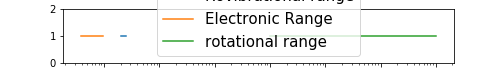
\includegraphics[scale=0.5]{images/chapter-1/ranges_of_transitions}
			\caption{Notice how the beam begins to diverge the further it travels away from the laser source. Lasers do not travel in straight lines because of an uncertainty law.}
			\label{fig:lase}
		\end{figure}

		This can be observed by comparing the laser spectrums of the isotopes of methane; CH4,CH3D, CH2D2, CHD3, and CD4. Upon examination, some peaks present in CH3D, CH2D2 and CHD3 spectrums are absent in CH4 and CD4 spectrums because of their structural differences. These differences arises because of the differing geometry of the isotopes. The total differences between isotopes are tiny relative to comparing differences between chemical species. With high enough resolution and sensitivity, we will be able to distinguish the minuscule differences between isotopes through these measured spectral properties. The spectral dependencies can be accurately predicted through the various levels of structure within atoms and molecules which are discussed subsequently. There is math behind all of this.
		
		Remember that molecules consists of elements and it is impossible to "photograph" them, so spectroscopy is our best method of characterizing atomic systems. The method of interaction discussed in this book typically include emission, absorption and dispersion of electromagnetic (EM) radiation with matter. Such interactions only occur when the frequency of the laser beam is resonant with an allowed transition of the atom or molecule. This interaction between the EM radiation and molecule is analogous to the resonance of harmonic oscillators of springs and mass systems. Transitions cause atoms and molecules to undergo a changes in their initial state[structure] of the wavefunctions[molecule] to another state[structure], be it higher for absorption or lower for emission. The method for determining which transition are allowed and disallowed will be discussed later on in the principles of spectroscopy.
		
		When determining the frequency range of interest, the atom or molecule and the type of transition must be considered so the appropriate type of laser and detector is used in the experiment. This is important as different types of transitions have differing degrees of coupling and ranges of frequencies. Degree of coupling typically effects peak strength. If coupling is poor, then the EM wave and atomic system do not resonate and no peak is observe for this transition. Strong coupling results in strong absorption and peaks. Electronic transitions involve changes in electronic energy of the electrons with transition frequencies ranging from visible light to ultraviolet. Rovibrational and rotational transitions requires electromagnetic frequencies from the infrared and microwave region respectively. In this book, we will be focusing on rovibrational spectroscopy of molecules and thus infrared frequencies of EM radition.
	
		\begin{figure} [!ht]
			\centering
			\def\svgwidth{\columnwidth}
			\resizebox{15cm}{!}{\imginput{images/abs-rovib-trans.pdf_tex}}
			\caption{Many of the molecules from the  diatomic species above have their vibrational mode  excited into its first vibrational excited state. This is caused by the absorption of the photon forming the laser beams. When energy from the photons, $qh\nu$, are transfered to the molecules, more intense vibrations of the molecules result.}
			\label{fig:abs-rovib-trans}
		\end{figure}	
		
		With molecules, we cannot make the assumption that the nucleus and/or electron within a molecule are non interacting like is for most of atomic spectroscopy. In molecules, atom are in such close proximity of each other because of bonding. These interaction must be taken into consideration in order to obtain reliable results. Some consequences of these interactions are shifts in the energy level of states due to mixing, various molecular conformations, their associated micro environments, coupling of modes of something something something (forgot the jargon) addition of rovibrational structure, and (talk about symmetry, man i really gotta brush up on this, super disgraceful). 

		\begin{figure} [!ht]
			\centering
			\def\svgwidth{\columnwidth}
			\Huge
			\resizebox{10cm}{!}{\imginput{images/laser-gaussian-beam.pdf_tex}}
			\caption{Notice how the beam begins to diverge the further it travels away from the laser source. Lasers do not travel in straight lines because of an uncertainty principle.}
			\label{fig:laser-gaussian-beam}
		\end{figure}
		
	\section{Introduction to Lasers and Optics}	
		\label{sec:Introduction to Lasers and Optics}
		So why are lasers so interesting? Why not broadband/divergent sources such as lamps? The  big reason for choosing to work with lasers is because of the potentials lasers have for ultrahigh resolution spectroscopy. It is a requirement which statistics and quantum mechanics proves. The techniques involved in creating and utilizing lasers are vastly more costly than broad band sources such as lamps. Which is better? That is answered entirely on the scope and application of ones purposes. The field that this book is written for is CEAS with highly refined spectrums. Resolutions high enough to observe hyperfine structure. Therefore a laser is a requirement. More simply put, we want high resolution so therefore we must use a coherent tunable lasing source.
		
%%include a figure and some discussion of "structure"
		
		Hyperfine structure results from interaction of nuclei and electrons within atoms and molecules, but is minuscule in comparison to rovibrational structure. Observation of hyperfine structure is not achievable with broadband sources of radiation because of how wide their linewidths are in comparison to lasers. Elaboration on this later. Lasers have naturally lower linewidths allowing for production of higher resolution spectrums as fine structures may be resolvable. Divergent radiation sources have much larger linewidths making them near impossible to observe hyperfine structure. People always come up with some clever technique or algorithm to overcome theoretical limitations however.
		
		\begin{figure} [!ht]
			\centering
			\def\svgwidth{\columnwidth}
			\resizebox{12cm}{!}{\imginput{images/linewidths-gaus-blackbody.pdf_tex}}
			\caption{The red line is a Gaussian beam with a frequency centered at about $5.0 \times 10 ^ {14}$ Hz  (600nm) while the blackbody radiation broadened over a large spectrum. The blackbody radiation source can be thought of as tungsten lamp, a broadband source. The frequency of the laser is very well defined in comparisons to the black body radiation source. This well defined frequency nature is what enables high resolution spectroscopic details to be extracted from a sample.}
			\label{fig:linewidths-gaus-blackbody}
		\end{figure}
				
		Despite this drawback, divergent radiation sources still have important applications where speed is essential, after all FTIR is still very relevant. Depending on which is more important, speed or resolution, the appropriate radiation source must be chosen. 
		
		Lasers nowadays are much more affordable and reliable now a days because of the advances in their technology (need to read up on lasers). Now is a good time to introduce the essential topics of lasers to classroom fields of study, not just in physics and chemistry. It is not necessary to go into full details about their derivation. Just enough knowledge to understand the properties of lasers an light sources and the technical skills necessary their operation is enough.
		
		For the topics in optics, this book will mostly cover linear optics and some of the effects of special crystals resulting in some non-linear optics. This book will discuss only the effects of the crystals, as the interaction between the crystal and laser beam is challenging. Nonlinear optics is an important topic however as non-linear crystals has allowed the implementation of many advance techniques such as modulation, heterodyning and tuning of lasers. It is not necessary to understand the above statements about non-linear crystals. Non-linear effects are taken for granted in this book. 
		
		\begin{figure} [!ht]
			\centering
			\def\svgwidth{\columnwidth}
			\resizebox{16cm}{!}{\imginput{images/non-linear-crystals.pdf_tex}}
			\caption{Examples of the modifications that can be performed on an input laser beams. These processes tend to be very inefficient in their conversions as the resulting output laser beams tend to be much lower in intensity than the input laser beams. Intensity is represented by the width of the beams. Not accurate, its just a cartoon.}
			\label{fig:non-linear-crystals}
		\end{figure}
		
	\section{Introduction of Tools to Learn}
		\label{sec:Useful Tools to Learn}
		The purpose of this section is to give a brief run down of how this book will help combine different platforms, programs and technologies into a functional system for a project. This book also aims to help improve current projects through good use of tools, techniques and coding. Most importantly, this book serves as a starting point to enlighten newcomers of research of what the community is, should, or could be using to design their projects. When considering project, one must think of the hardware, the language, the program, and the environment where the project is based. To help illustrate how to design a project, this book will look at the early stages of the Gaussian Beam Profiler (GBP) project.
		
		\begin{figure} [!ht]
			\centering
			\def\svgwidth{\columnwidth}
			\Huge
			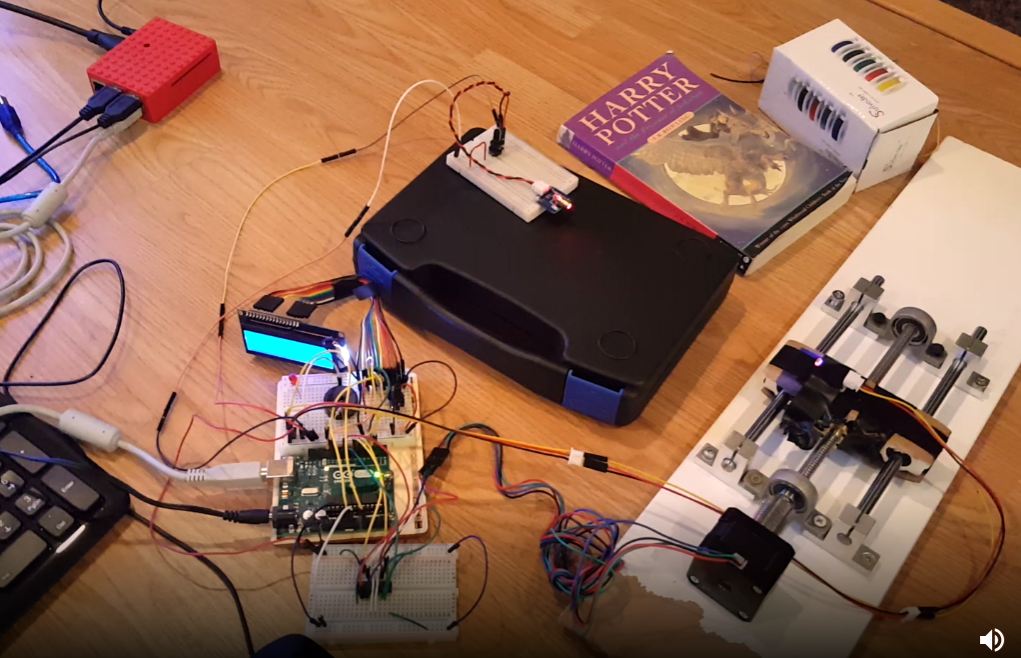
\includegraphics[scale=0.35]{images/chapter-1/internet_of_things_for_project}
			\caption{Here is an early build of the project when it was a do it at home project. The Raspberry Pi is running UbuntuMate and is used to signal the Arduino and collect, store and process the incoming data from the Arduino. The Arduino controls the motor, the LCD screen, the laser and the piezo buzzer. The motor is attached to the optical axis moving the detector along a horizontal axis across the beam. }
			\label{fig:internet_of_things_for_project}
		\end{figure}
	
		A key aspect of any project or experiment is its purpose. Any laser spectroscopy project requires a laser and a detector to measure the beam. To profile a beam, we need at least one axis where the detector can move about, leading us to use an optical axis with a step motor. Since we are doing find discrete measurements, a step motor with small steps are ideal. To handle the sensors, detectors and motor control, an Arduino board was used because of its quick response and stability. To signal and provide a GUI for an individual to work with, Raspberry Pi with UbuntuMate was utilized. A regular laptop would suffice, but it was a Internet of Things project. Once we have all the components required, we are ready to plan how to control the experiment. Control broadly means data storage, processing, visualization and communication between the various components of the project. Communication between everything was achieved serially, a basic but adequate system of communication for this simple project. In a professional environment, a more complicated system may instead use national instruments, drivers, and LabView to achieve everything. Which is better? That depends on the individual and work environment. This was a do it an home online class project so I used the two boards used in the class.
			
		For this simple project, data storage, processing and visualization is handled by Python and the packages numpy, matplotlib, sqlite and pyserial. Numpy and matplotlib were used to process and plot the data while sqlite is used as a database to store the data. Since the decide protocol was serial, we used pyserial packages to handle the serial communication between the Arduino and the python program  running on the Raspberry Pi. This may take a bit for beginners to comprehend, but that is what this book is for. It is important for students to be familiar with Python and its commonly used packages. Knowing how to use serial is only necessary if you are involved with the designing and engineering of the project. It would be recommended to be capable of utilizing all these packages without external help. For some however, understanding the capabilities of the tools available on Python is adequate.
		
		Before delving into what the Arduino is doing, it would be helpful to somewhat formally explain what serial communication is. Serial communication is a protocol where data is transmitted between two devices, leading to communication. A section on serial is not in this book and a protocol is a set of rules forming some standard. By adhering to some standard such as serial, devices can be made to communicate with one another no matter the place, time, manufacturer and type of component they posses. There are resources online describing the protocols or rules of serial communication. All that matters for the end user is the importance of frequency or baud rate must be the same in order for the two to communicate which is analogous to channels in radio work. Not all components in the system have to be on the same baud rate, but at least two must be. Serial is one of the simpler types of communications to implement into a system, but it suffices for most projects. This book will not delve into how communication of the internet works but this book will discuss how to use Python to communicate on the web. Just like serial communication, communication over the internet requires protocols which devices must adhere by to connect to the internet. 
		
		Now that a brief discussions of serial and communication has been developed, discussion of communication between the Arduino, Raspberry Pi python program and LCD screen can begin. The communication between the Raspberry Pi and Arduino and the Arduino with the LCD are kept seperate. Despite the Arduino being the common component between the two connections and the baud rate being the same between all components, timing of the signals must be very well defined to ensure all the code and components run well. Ie to avoid disaster. This is a crucial thing to keep in mind when creating the programs as a significant portion of the time debugging will be spent figuring out an optimal timing for the programs. The coding can get messy because serial must be enabled by python in the Raspberry Pi while serial is enabled by the Arduino editor. The two languages are different adding to the complexity. 
		
		\begin{figure} [H]
			\centering
			\def\svgwidth{\columnwidth}
			\Huge
			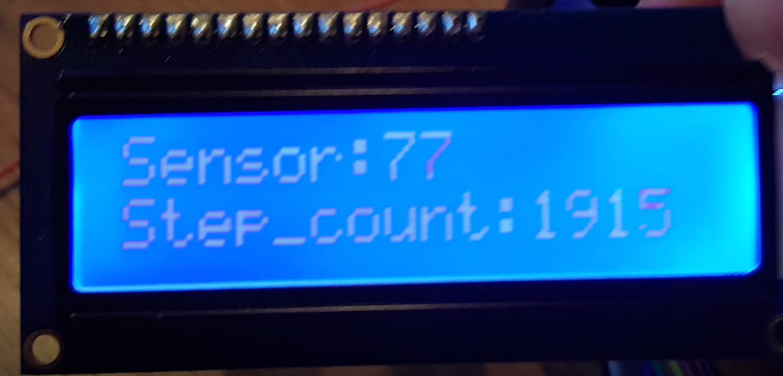
\includegraphics[scale=0.20]{images/chapter-1/detector_real_monitor_lcd_display}
			\caption{An LCD display is being used to display the step count and the detector value. Achieved through serial communication between the LCD and Arduino.}
			\label{fig:detector_real_monitor_lcd_display}
		\end{figure}
	
		\begin{figure} [!ht]
			\centering
			\def\svgwidth{\columnwidth}
			\Huge
			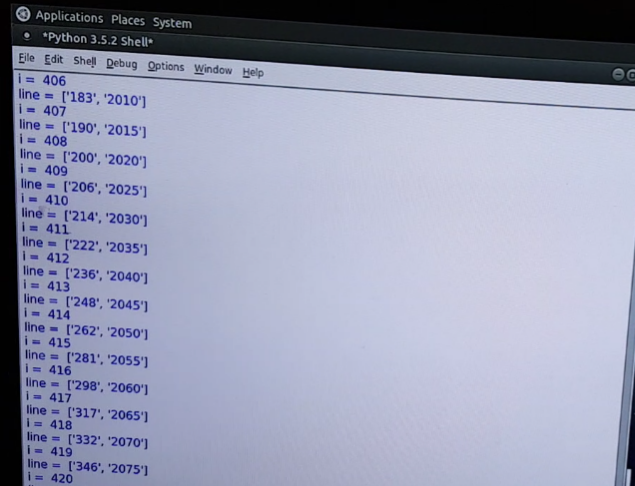
\includegraphics[scale=0.40]{images/chapter-1/data_collection_python_serial}
			\caption{The python program on the console is retrieving the detector value and sensor count from the Arduino serially. The data is then stored in an SQLite database every so steps.}
			\label{fig:data_collection_python_serial}
		\end{figure}	
		
		\begin{figure} [!ht]
			\centering
			\def\svgwidth{\columnwidth}
			\Huge
			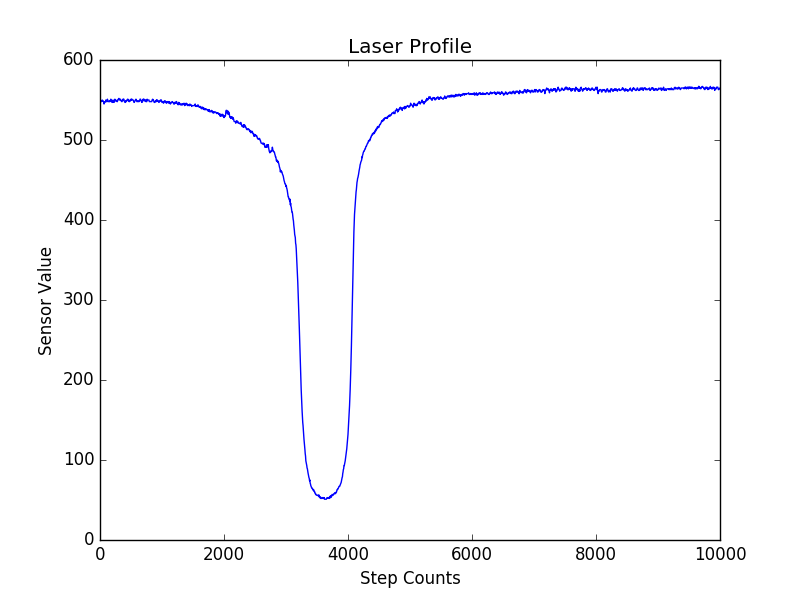
\includegraphics[scale=0.60]{images/chapter-1/sample_plot_data_with_sql_numpy_matplotlib}
			\caption{From the database, data is taken from the database and loaded into python for data processing and visualization with numpy and matplotlib. The image shows the intensity of the beam along a 1D axis}
			\label{fig:sample_plot_data_with_sql_numpy_matplotlib}
		\end{figure}
		
		After progressing the project to state as shown in the image, new coding was implemented into the system to allow a joystick to initialize the position of the detector and begin the scan. This was mostly because of good coding, no additional expensive hardware was added to the system other than a joystick. To do required good timing and communication between the Arduino and Python which was extremely tedious to set up. Alternatively, LabView could easily have done the same job but with digital buttons in the program. There is always more than one solution to a problem, what matters is that you can use what is available for the project.
		
		\begin{figure} [!ht]
			\centering
			\def\svgwidth{\columnwidth}
			\Huge
			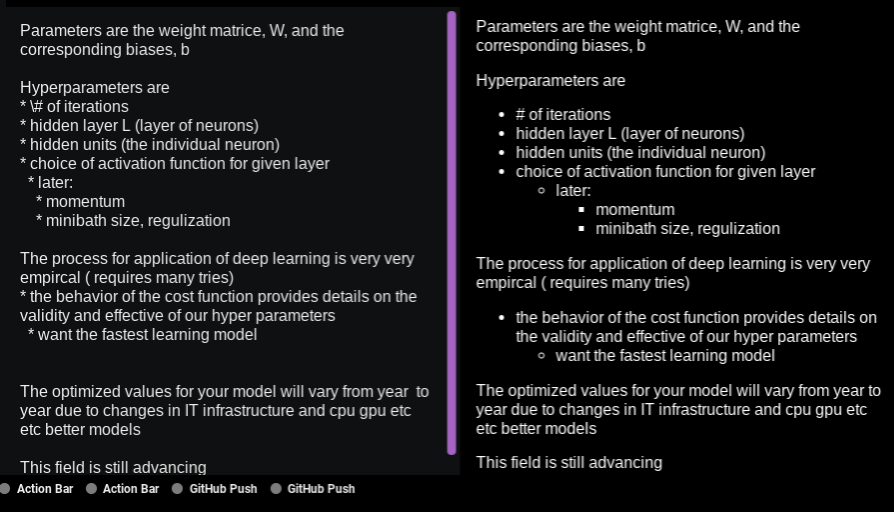
\includegraphics[scale=0.45]{images/chapter-1/markdown_of_machine_learning}
			\caption{This is markdown example of a machine learning notes. On the right is the "code" of the document while the right is the resulting document.}
			\label{fig:markdown_of_machine_learning}
		\end{figure}		
		
		Markdown is an incredibly simple tool for making simple structured documents quickly. It takes about 5-10 minutes to grasp how to create MarkDown documents and there are plenty of references to look at to get the document doing what it is required to do. MarkDown however is not a suitable language for creating journals or books. It is more for notes of presentations. To create journal articles and documents, LaTex is the go to system. This book, despite being made in LaTex, will not go over it however.
		
		\begin{figure} [!ht]
			\centering
			\def\svgwidth{\columnwidth}
			\Huge
			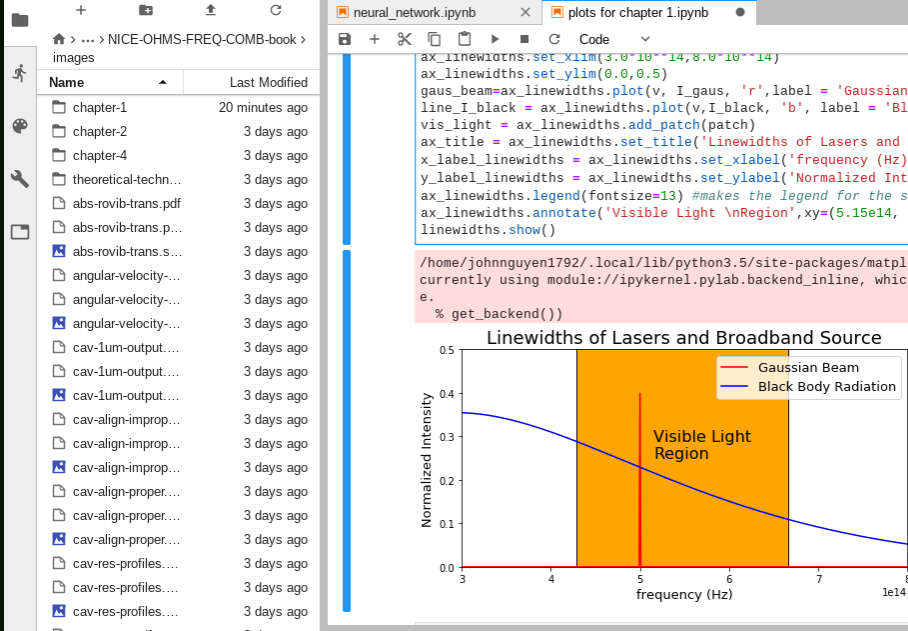
\includegraphics[scale=0.45]{images/chapter-1/jupter_image_plot_program}
			\caption{Jupyter is a project that enables the use of Markdown, Python and other languages on a single platform. This makes it an ideal platform for working, taking notes, data processing, presentations and data visualizations.}
			\label{fig:jupter_image_plot_program}
		\end{figure}
	
		Finally, making diagrams that quickly and elegantly explain things visually is a very valuable skill. Many of the figures in this book were created using Inkscape and/or Python. With these masterful figures, this book is able to speak less and show more with simple but to the point diagrams. There are a lot of components to the SVG images used in this book, but they will not be covered as the their method of implementation is still painful and very likely to change.
		
		That was a lot for an introduction, but having a brief semi holistic introduction to the tools and its uses should greatly help newcomers to the scene as research is incredibly overwhelming. This is especially true when guidance from a mentor or senior may not be available.
	\section{Basic Direct Absorption Spectrosopy Setup}
		\label{sec:Basic Direct Absorption Spectrosopy Setup}
		With all these topics of spectroscopy, optics, engineering, and computer skills in mind, we want to build a simple spectroscopy experiment to collect an absorbance signal from the sample. The aim when creating any system should be automation to reduce error, downtime and increasing efficiency. Effectively, we freeing up as much time as possible for the experimentalists so that they  can focus on performing more complex tasks that require flexibility and creativity of the human mind. The setup should be built so that anyone can turn on the system, effortlessly begin data collection and followed by data analysis to produce your lovely spectrum or signal.To illustrate this outline, the direct absorption spectroscopy figure will be used as a demonstration. 
		
		To follow \autoref{fig:dir-abs-spec-setup}, start at the laser source and follow the laser and signal all the way to the computer with the spectrum while reading the annotations in order.	
		
		\begin{figure} [!ht]
			\centering
			\def\svgwidth{\columnwidth}
			\resizebox{16cm}{!}{\imginput{images/dir-abs-spec-setup.pdf_tex}}
			\caption{This image illustrates a basic direct absorption spectroscopy setup with all the essential components.}
			\label{fig:dir-abs-spec-setup}
		\end{figure}	
		
		\noindent
		{\bfseries (A)} The optical system is used to adjust the beams various parameter such as intensity, phase and frequency.\\
		{\bfseries (B)} At least two mirrors must be used to perform fine tuning of the laser in 3 dimensions. This is necessary in order to propagate the beam through the sample and detector crystal. \\
		{\bfseries (C)} As the beam travels through the optical system, there is power loss at various point of the laser beam. Substantial loses occur at the optical system. At\\ {\bfseries ***}, the is beam split so that the a laser intensity can be approximated. The most important location of power loss is at our sample as that is where our signal lives.\\
		{\bfseries(D)} The detector analog signals travels to the USB-DAQ with some modification to the signal if necessary. The USB-Daq then converts the analog signals into digital so that can be transferred to a computer to be stored and processed. \\
		{\bfseries(E)} More than one program can be used in the data collection and processing. For example, Labview can be used to initiate communication with the instruments, such as the laser, and initiate the USB-Daq for data acquisition. The generated data file can be loaded on to IPython console, Jupyter notebook, or Igor for automated data manipulation and plot creation.		
	
	\section{Advance Techniques}
		\label{sec:Advance Techniques}
		The rest of the content will begin to increase in complexity as we focus on more relevant spectroscopy techniques such as frequency modulation spectroscopy, Pound-Drever-Hall locking technique, cavity enhanced absorption spectroscopy, frequency combs, noise immune cavity enhanced optical heterodyne molecular spectroscopy, and something something.

%-------------------------------------------------------------------------------%
%-------------------------------------------------------------------------------%
%-------------------------------------------------------------------------------%
\part{Spectroscopy}
\chapter*{Introduction}
	In this part of the book, the fundamentals of absorption spectroscopy is developed by the use of quantum mechanics and classical mechanics. Unlike the optics part of the book, this part on spectroscopy develops a bit of the theory as molecular species vary greatly. Now a days, there are computer algorithms that can accurately describe the energy levels and signals that are measurable with laser absorption spectroscopy however the details provided by the computer simulations are shallow. In order to truly understand a molecule, a deep model of it must be created. Hence why this part of the book goes over the derivation of signals of methyl radical. From this part of the book, one should gain the ability to create their own complex model for their targeted species for deeper analysis. Every part of spectroscopy from the absorption, energy levels, shape of the signals, and quantum numbers of rovibrational laser absorption spectroscopy.
	
\chapter{Fundamentals of Spectroscopy}
	\label{chp:Fundamentals of Spectroscopy}
	
	\begin{figure} [!ht]
		\centering
		\Large
		\def\svgwidth{\columnwidth}
		\resizebox{13.5cm}{!}{\imginput{images/particle-wave-duality.pdf_tex}}
		\caption{{\bfseries Particles} behave just like any old soccer ball, they collide and reflect off surfaces. \newline
			{\bfseries Waves} can diffract, become attenuated in intensity, and interfere with each. \newline
			{\bfseries Microscopic particles} such as electrons and photons show both characteristics.}
		\label{fig:particle-wave-duality}
	\end{figure}
	
	Spectroscopy is the field where atoms and molecules are experimentally probed to obtain spectral information for characterization. There are a number of techniques currently employed to obtain spectroscopic detail of the target species, such as Resonance-Enhanced MultiPhoton Ionization and mass spectroscopy. This book will focus on the class of Laser Absorption Spectroscopy (\autoref{sec:Laser Absorption Spectroscopy}) techniques for observations of possible transitions in quantum systems. With frequency ranges in the infrared to microwave, molecular transitions involving rovibrational and rotational are observed. Rovibrational spectrums of provide structural details of molecules such as the bonding order between the elements, conformational structure and isotopic information. 
	
	Before jumping into infrared spectroscopy, it is necessary to discuss the quantum mechanics behind the molecular interaction with electromagnetic radiation, as shown in (\autoref{fig:photon-electron-transition}), in order to lay out the foundation for understanding spectroscopy. The proofs are simplified since this is not a quantum mechanics textbook. The classical electromagnetic radiation will now be treated as the quantum mechanical photon in this chapter for convenience. 
	
	\begin{figure} [!ht]
		\centering
		\Large
		\def\svgwidth{\columnwidth}
		\resizebox{12cm}{!}{\imginput{images/methyl-radical.pdf_tex}}
		\caption{{Methyl Radical (CH3) radical. It is like methane (CH4), a tetrahedral molecule, but is missing a hydrogen bond. It is a radical species with a lone electron. It is also neutral in charge.}}
		\label{fig:methyl-radical}
	\end{figure}
	
	At the microscopic level, matter exhibits both particle and wave like properties (\autoref{fig:particle-wave-duality}). This is known as the particle-wave duality. For slow and microscopic systems, wave like properties dominate over the particle like behavior. This is referred to as the quantum limit where the wave nature of matter allows for the treatment of the classical particle as a wavefunction. Some properties due to the wavelike nature are the discreteness of wavefunctions an their energies, the probabilistic behavior of the particle, and the uncertainty of various measurable quantities. The tunneling nature of particle's will be overlooked in this book. 
	
	What is a wavefunction? A wavefunction is a mathematical construct describing the state and properties of the system in a wavelike fashion. The system can be a single particle, a molecule, a group o molecules and so forth. From the wavefunction and the use of mathematical operators, abstract spaces/groups with non visualizable dimensions, statistics, probability, complex planes and other math techniques, we can create, interpret and derive meaningful physical results. This is the foundational proof that quantum mechanics is fundamental law in this universe. The quantum mechanics and the derivations are rigorous, but we focus only on the necessary concepts to interpret spectroscopy. It is important to note that wavefunctions are not physical and are mathematical constructs that exist in the complex plane. If all of this is confusing, do not worry as this information is to provide directions for those who are interested in the complexity of quantum mechanics.
	
	From the wavefunction, we can infer various information describing the behavior of the system, such as the energy, location, momentum, angular momentum, and so forth. The exact form of the wavefunctions must satisfy the Hamiltonian with the associated boundary conditions of the problem.
	
	\begin{eqnarray}
		\label{eq:hamiltonian of wavefunction in cartesian}
		\hat{H} (x, y, z) \psi(x, y, z)
			&=&\left( \hat{T}(x, y, z) + \hat{V}(x, y, z) \right) \psi(x, y, z)\\
			&=&E\psi(x, y, z)
	\end{eqnarray}
	
	\begin{figure} [!ht]
		\centering
		\large
		\def\svgwidth{\columnwidth}
		\resizebox{15cm}{!}{\imginput{images/photon-electron-transition.pdf_tex}}
		\caption{{\bfseries (A)} The electron in the 1s state is absorbing an electron and transitioning into the 2p state which is higher in energy. 
		\newline
		{\bfseries (B)} The 2p electron lowers to the ground state 1s electron while also emitting a photon. \newline
		\textbf{Note:} If the absorption and emission process occur sequentially and the electron is the same in both transition, the emitted photon is randomly scattered in any direction.}
		\label{fig:photon-electron-transition}
	\end{figure}	
		
	\noindent
	The Hamiltonian operator, $\hat{H}(x,y,z)$, is the energy operator and can be thought of as "acting on" a wavefunction, $\psi(x, y , z)$, to obtain the energy of the wavefunction as an eigenvalue. The eigenvalue is the constant pulled out in front of the wavefunction after the operator has operated on the wavefunction. From classical mechanics, we know that there are two types of energy, kinetic and potential energy. The Hamiltonian operator, analogous to the classical interpretation of energy, also consist of two operators itself; the kinetic energy operator ($\hat{T}$) and potential energy operator ($\hat{V}$).
	
	No wavefunctions equation will be "shown", but instead will be represented by their bra and ket form for simplicity. $\ket{\psi_k}$, $\bra{\psi_i}$ and $\braket{\psi_i|\psi_k}$ or $\ket{k}$, $\bra{i}$ and $\braket{i|k}$. In order to generalize, coordinates are not shown as the coordinate system used to solve the problem will depend on the symmetry of the Hamiltonian. This is because the symmetry of the potential energy operator $\hat{V}$) is what determines the symmetry of the wavefunctions. Higher importance will be shifted on to the operators, quantum numbers and eigenvalues.
	
	\begin{eqnarray}
		\label{eq:hamiltonian of wavefunction in braket notation}
		\hat{H}(x, y, z)\ket{\psi(x, y, z)}
		&=&\left( \hat{T} + \hat{V}\right) \ket{\psi_i}\\
		&=&E_i\ket{\psi_i}
	\end{eqnarray}
	
	When a particle is confined by bonding, high energy barriers, or any physical constraints, the wavefunction of the particles begin taking on discrete forms. This discreteness means that the wavefunction either looks like a cat, a dog, or an elephant, not a chimera. This confinement on the wavefunction is represented by the potential operator, $\hat{V}$. The form of the discreteness originates from the applied boundary conditions on the Hamiltonian function or more generally, the partial differential equation. The discrete forms are better known as the {\bfseries state} and {\bf quantum numbers} of the wavefunction. Examples of systems with discrete states are the electrons bound to a positive nucleus resulting in the $ n = 1, 2, 3, 4 ... \infty $ electronic energy levels of the electrons, discrete vibrational and rotational states of molecules, and allowed resonating frequencies of photons of an optical cavity \autoref{sec:Optical Cavity and Resonance Properties}. Note that a free running electron does not posses "electron orbitals" nor does a unconfined photon have modes.
	
	%make diagram of rovibrational energy levels
	
	Transitions from one state to another can be caused by the absorption or emission of photons. With the absorption of a photon, the system increases in energy because of the transition from a lower energy state to a higher energy state. For emission processes, the system transitions into a lower energy state while emitting a photon. The processes are essentially a forward and reverse pair. These transitions between the wavefunctions are also discrete, meaning only photons of specific energy may be absorbed or emitted. The energy difference for the transition is equal to the energy of the photon that is absorbed or emitted. The energy of a photon is determined by its frequency or wavelength where higher frequencies and lower wavelengths correspond to photons with higher energy. This energy relation is given by \autoref{eq:photon energy forms}. The last form of photon energy is in terms of wavenumbers which we will be using the most.
	
	\begin{equation}
		\label{eq:photon energy forms}
		\begin{array}{cccccccc}
		E_{photon}=h\nu=\hbar \omega &\qquad &E_{ik}=E_{k}-E_{i}  & \qquad & E_{ik} = E_{photon}& ||| &\tilde{E}=h\tilde{\nu}
		\end{array}
	\end{equation} 
	
	Quantum numbers can have a finite or infinite set of states. Examples of finite quantum numbers are the electron or nuclear spin states. For quantum numbers with infinite sets, there are the vibrational, rotational and electronic states of molecules. Mathematically, this means that these wavefunctions or solutions, for a given Hamiltonian or partial differential equation, form an infinite dimensional orthogonal basis set in their Hilbert space. It is normal to have an infinite number of states as long as the occupation probability of the higher level states drops to zero as the energy of the wavefunction increase. This means that the weight or importantness of higher energy states become negligible as their energy increases.
	
	If there are an infinite number of states, then there should be an infinite number of transitions. Thankfully, there are a finite number of \textbf{observable} transitions because of how we are detecting these transitions. Interpreting spectrums of molecules would be impossible if all possible transitions were observable. Mathematically, this finiteness of observable transitions is because of the symmetry of the wavefunctions, electromagnetic radiation perturbation, statistical distribution of the states, and selection rules. In short, not all transition between states are allowed.
	
	An example of a simulated statistical distribution of states is shown in \autoref{fig:Methyl-Radical-Angular-Momentum-Distribution}, which describes the thermal equilibrium population of rotational states for methyl radical. As the total and component angular momentum of the state increases, the population of these states quickly decrease to zero. This is an example of higher energy states losing their importance despite their energy increases. The transitions involving these high angular momentum states are less observable since there are few radicals populating these states to begin with. There is also the consideration of energy degenerate states. The relation between energy, probability and statistical distribution of states will be explained in %\autoref{subsec:Statistical Distribution}. 
	
	\begin{figure} [!ht]
		\centering
		\Large
		\def\svgwidth{\columnwidth}
		\resizebox{14cm}{!}{\imginput{images/Methyl-Radical-Angular-Momentum-Distribution.pdf_tex}}
		\caption{Methyl radical angular momentum distribution with 2 quantum numbers. Methyl radical belongs to the C3V point group.}
		\label{fig:Methyl-Radical-Angular-Momentum-Distribution}
	\end{figure}
	
%-------------------------------------------------------------------------------%
%-------------------------------------------------------------------------------%
	\section{Infrared and Microwave Spectroscopy}
		\label{sec:Infrared and Microwave Spectroscopy}
		Till this point, the distinction between \underline{\textbf{rovibrational}} and \textbf{rotational} spectroscopy has been made, but not explained. The two are different types of spectroscopy, but are interconnected. This is because \underline{\textbf{rovibrational}} spectroscopy is spectroscopy of \underline{vibrational} states coupled with \textbf{rotational} states. There is no \underline{vibrational} spectroscopy since the coupling is inherited through the nature of the transitions. \underline{\textbf{Rovibrational}} spectroscopy also involves broader peaks in comparison to \textbf{rotational} spectroscopy. The broadening is a result of \underline{\textbf{rovibrational}} spectroscopy having higher energy transitions and possessing a larger distribution of states. The relationship of energy and broadening is because of an uncertainty principle which will not be discussed.
		
		Rotational spectroscopy is the more fundamental spectroscopy of the two spectroscopies. This means that its distribution of states only consists of the \textbf{rotational} quantum numbers, while \underline{\textbf{rovibrational}} distribution involve the distribution of the \underline{vibrational} mode and \textbf{rotational} quantum numbers. To prove how quickly distributions can broaden as we include more quantum numbers, we look at the following dice and deck of card analogy. 
		
		Consider a 6 sided dice and a deck of cards. Individually, a 6 sided die has 6 outcomes while a full deck of card has a 52 outcomes. There are 312 outcomes when considering both the dice and deck. The number of the outcomes for both the dice and deck is much larger then the number of outcomes of the dice and deck individually. If a 1 rolled, there are 52 different cards to draw from. Some outcomes include, rolling a 1 with a Ace of Spades, rolling a 1 with a 5 of Hearts or rolling a 1 with the Queen of Clubs. The outcome of rolling a 2, 3, 4, 5, or 6 while drawing any of the 52 cards are also possible. The complete set of possible combination of cards and dice rolls is known as a distribution. This distribution of the dice and deck of card is much larger than the distribution of the dice or deck of cards alone. This concept can be applied to our molecule with \underline{vibrational} states being represented by the dice and \textbf{rotational} states being represented by the deck of cards. Because \underline{\textbf{rovibrational}} spectroscopy involves \underline{vibrational} and rotation states, \underline{\textbf{rovibrational}} spectroscopy is inherently broader than \textbf{rotational} spectroscopy which includes only \textbf{rotational} states.
		
		Unlike the card and dice analogy, there exist a larger combination of states belonging to the \underline{\textbf{rovibrational}} and \textbf{rotational} quantum numbers. This larger spread of the distributions of states between \underline{vibrational} and rotation states causes \underline{\textbf{rovibrational}} spectroscopy to be exponentially more complex than \textbf{rotational} spectroscopy. The same can be said for electronic spectroscopy in comparision to \underline{\textbf{rovibrational}} spectroscopy. This is also a causes of peaks from \underline{\textbf{rovibrational}} being more broadened in comparison to \textbf{rotational} spectroscopy. Rovibrational spectroscopy becomes even more complex when energy coupling of \underline{vibrational} and \textbf{rotational} numbers are taken into account. 
		
		In the case of methyl radical, there are two quantum numbers associated with angular momentum as seen in \autoref{fig:Methyl-Radical-Angular-Momentum-Distribution}. These two quantum numbers are labeled the total and component angular momentum which will be discussed shortly. The odd shape of the distribution is a result of the component angular momentum of methyl radical having a finite number of states/dimensions while the total angular momentum being infinitely dimensional. %There is a 3rd quantum number M which is the projection of J onto the z axis. The 3rd quantum number will be developed in a later section.
		
		The role that the various combination of states play on resolution will be covered in \autoref{sec:Factors in Resolution}. As aside, electronic spectroscopy includes coupling with a larger set of quantum numbers and thus larger distribution of combinations. Electronic states requires working with electronic, \underline{vibrational} and \textbf{rotational} states. This makes electronic spectroscopy exponentially more complicated than \underline{\textbf{rovibrational}} spectroscopy. A positive note on electronic transitions are the abundance of lasing sources, detectors and components available for electronic spectroscopy. This is because working with the visible frequencies is much easier than with invisible frequencies thus resulting in the field of visible frequency being far more developed. Hopefully, the idea of the best and worst is being replaced by pros and cons.
		
%-------------------------------------------------------------------------------%
%-------------------------------------------------------------------------------%
	\section{Rovibrational Spectrocopy}
		\label{sec:Rovibrational Spectrocopy}
		%talk about gas phase
		
		%include rovibrational energy transitions spectrums etc diagrams.
		When developing rovibrational spectroscopy, it is common to use a simple diatomic as a model before moving onto more complicated systems. For efficiency however, we will jump right in to developing the principles of rovibrational spectroscopy using methyl radical model. We start with methyl radical since it belongs to a less symmetric point group, has more modes of vibrations and there are plenty of spectroscopy books that begin developing the principles of spectroscopy with diatomics. It also would be redundant to go through the derivation for a diatomic molecule and then again for a slightly more complicated polyatomic. The principle theory for quantifying the spectral properties of diatomics is already inherent in any polyatomic system with added complexity from the increase in degrees of freedom. Luckily, this increased complexity is greatly simplified with group theory. For teaching purposes, this allows us to treat group theory on the same footing as perturbation theory and selection rule.
		`
		One of the dilemma when working with molecules of lower symmetry point groups (subgroup) is the increased number and size of quantum numbers or modes required to describe the properties of the system. As shown in \autoref{fig:Methyl-Radical-Angular-Momentum-Distribution}, a 3d statistical distribution is required to represent the angular momentum for methyl as there are two quantum numbers for describing its angular momentum. A linear diatomic would have a 1 dimensional plot describing its distribution rotational state. This is classically equivalent to saying two degrees of freedom are required to describe the rotation of the system. With diatomics, there is only 1 quantum number. For larger complicated molecules, there are at most 3 quantum numbers for rotational spectroscopy analogous to how 3 degree of freedom belong to rotation for large bodied systems. The remaining degrees of freedom go into describing the vibrational modes. The last part should be familiar to those who have studied classical mechanics. This connection of degrees of freedom and quantum numbers allows us to conveniently use results from classical mechanics as opposed to solving the true wavefunction of the system. The wave equation of large systems tend to be very difficult, if not impossible, to solve so recognizing the connection between classical mechanics and quantum mechanics allows us to solve and characterize otherwise impossible systems.
%-------------------------------------------------------------------------------%		
		\subsection{Rotational Spectroscopy}
			\label{subsec:Rotational Spectroscopy}
			Before determining the rovibrational spectrum of methyl radical, we first need to calculate the rotational energy levels. Assuming no prior knowledge of the bond lengths and angles within methyl radical, we can only approximate the energy using some initial input parameters for bond lengths and angles. When constructing the rotational Hamiltonian model of methyl radical, there are a some things that must be kept in mind. We do not solve the Hamiltonian for the rotational wavefunction, but are still able to obtain the rotational eigen energies. There is a relatively simple method of obtaining the rotational energy level of any molecule that involves using techniques and results from classical mechanics. This is accomplished by changing frames and choosing a new axis system. This method is applicable to all molecules and simplifies the problem in comparison to solving Hamiltonian of the system by brute force.	Since we are dealing with only angular momentum, ie spinning systems, it is natural to use spherical coordinates because we want the variables to be separable and in 3 dimensions. Cartesian coordinates would require complex calculations and would still result in identical results, if solvable. It is advisable to stay away from using the Cartesian coordinate system, but trying to solve the rotational motion with Cartesian coordinates would provide practical experience as to why it is recommended to solve problems using the "correct" coordinate system. Mathematically, the logic would follow like \autoref{eq:setting-up-hamiltonian} below.
			
			\begin{eqnarray}
				\label{eq:setting-up-hamiltonian}
				\hat{H} (x, y , z) \ket{\psi_i(x, y , z)} 
				&\rightarrow&
				\hat{H} (r,\theta, \phi) \ket{\psi_i(r,\theta, \phi)}
				\\
				\hat{H} (r,\theta, \phi) \ket{\psi_i(r,\theta, \phi)} 
				&=& 
				E_i\ket{\psi_i(r,\theta, \phi)}
			\end{eqnarray}	
			
			The Hamiltonian operator we are interested in is the rotational Hamiltonian, \autoref{eq:rotational Hamiltonian 1}
			
			\begin{equation}
				\label{eq:rotational Hamiltonian 1}
				\hat{H}_{rot} = \dfrac{\hat{L^2}}{2I}
			\end{equation}
			
			$\hat{L}$ is the total angular momentum operator which contains the azimuthal term of the kinetic energy operator term. Do not worry if that made no sense. This is just  mathematical way of saying that our solutions are of the spherical Harmonics and that our solutions are of the form $l(l+1)$. We will not solve for the wave solution. We only consider the kinetic energy terms due to rotation in this section since we assume that translation and rotational motion of the molecule are separable. This is always true in fact. 
			
			The overall process is to determine the center of mass frame, calculate the inertia tensor in this new frame, diagonalize the inertia tensor to produce a diagonal matrix and solve for the rotational energy in the Hamiltonian \autoref{eq:rotational Hamiltonian 1}. 			
			
		\subsection{Center of Mass Frame}
			\label{subsec:Center of Mass Frame}
			
			\begin{figure} [!ht]
				\centering
				\Large
				\def\svgwidth{\columnwidth}
				\resizebox{14cm}{!}{\imginput{images/center-mass-frame-transformation.pdf_tex}}
				\caption{Transformation from some initial frame to the center of mass frame.}
				\label{fig:center-mass-frame-transformation}
			\end{figure}	
			
			The first step to solving the rotational energy levels is to layout the molecule in an initial frame and then proceed to transform it in to the center of mass frame. The center of mass is the point where the mass of the entire system can be localized so that the systems reactions to external forces and torques are simplified. When determining the center of mass frame, if possible, choose an initial frame that is close to where the center of mass frame is. For simple symmetric molecules, it should be easy to estimate. In the case of methyl radical, the center of mass must be between the carbon and 3 hydrogen atom. The carbon is more massive than the 3 hydrogen atom, therefore it must be closer to the carbon. A good choice is to place the initial origin at the center of the carbon atom then align the principle axis of the molecule along the z axis. Then placing one of the hydrogen atoms placed along the x or y axis to ease the calculation a bit in this step and in the next inertial tensor step. This is shown step by step in \autoref{fig:center-mass-frame-transformation}. With the coordinates of the carbon and 3 hydrogen atoms now declared, we begin calculating the center of mass using equations \autoref{eq:total mass} and  \autoref{eq:Center of Mass}.
			
			\begin{equation}
				\label{eq:total mass}
				M = \sum_i^4{m_i}
			\end{equation}
			
			\begin{equation}
				\label{eq:Center of Mass}
				R_{cm}=\dfrac{1}{M}\sum_i^4{m_ir_i} 
			\end{equation}

			After determining the center of mass in the initial frame \autoref{fig:center-mass-frame-transformation} (A), we shift the entire system by $-R_{cm}$ so that the center of mass is now the origin. In this new coordinate system, the rotational motion is one step closer to being separable.
			
%-------------------------------------------------------------------------------%
		\subsection{Angular Momentum and Velocity}
			\label{subsec:Angular Momentum and Velocity}		
			Angular velocity and angular momentum are similar in concept to velocity and momentum, but are used to describe the rotational quantities of a system as opposed to the translational quantities. The easiest interpretation of angular velocity is to describe it as the rate of which the angle of a body changes with respect to its rotation axis. If a ball is spun on a finger, then the direction which the finger points is the rotation axis. The motion of any point of the ball is perpendicular about a plane which is parallel to the floor. Formally, angular velocity is defined as \autoref{eq:angular velocity} below.
			
			\begin{equation}
				\label{eq:angular velocity}
				\vec{\omega} = \dfrac{\vec{r} \times \vec{v}}{|r|^2}
				= \braket{\omega_x,\omega_y,\omega_z}
			\end{equation}
			
			This quantity is a vector, meaning it has a magnitude and a direction. The ball could spin about any plane or along any axis within our coordinate system. More information on vectors can be found in the theoretical techniques chapter at \autoref{sec:Vectors and Dual Vectors}. The $\vec{r}$ is the position vector of some point of interest relative to the origin. For the molecule, we redefined the origin to be the location of the center of mass. The $\vec{v}$ vector describes the direction of which the ball is traveling. The ball as a whole is not moving anywhere, but a given point on the ball definitely has some velocity.
			
			\begin{figure} [!ht]
				\centering
				\def\svgwidth{\columnwidth}
				\resizebox{16cm}{!}{\imginput{images/angular-velocity-momentum.pdf_tex}}
				\caption{\textbf{(A)} The angular velocity of the ball is in all 3 direction. \\
				In \textbf{(B)} \textbf{(C)} and \textbf{(D)}, the component angular velocity of \textbf{(A)} in the x, y and z direction are shown respectively. From left to right, the rotational energy of the balls increase. \\
				\textbf{(D)} The direction of the angular velocity vector, $\omega_z$ are in the z direction. The spinning motion is about the x and y plane.
					}
				\label{fig:angular-velocity-momentum}
			\end{figure}	
					
			Angular momentum is a more abstract quantity and concept in comparison to angular velocity and translation momentum. Although it is the rotational analog of translation momentum, $mv$, angular momentum is usually not in the same direction as the angular velocity. The best definition that this book will make about angular momentum is that angular momentum is the response an inertial body has to angular velocity. Different inertial bodies with different inertia tensors will respond differently to the same angular velocity.
			
			\begin{equation}
				\label{eq:angular momentum}
				\vec{L}=\textbf{I}\vec{\omega}
				=\braket{\text{I}_{x}^x\omega_x,\text{I}_{y}^y\omega_y,\text{I}_{z}^z\omega_z}=\braket{L_x,L_y,l_z}
			\end{equation}
			
			$\textbf{I}$ is the inertia tensor of a body which is described in \autoref{subsec:Inertia Tensor}. Angular momentum is a very important quantity despite its poor definition since rotational energy of an object is dependent on angular momentum. It is also highly important due to being a conserved and observable quantity in quantum mechanics. The following relationship between rotational energy and the rotational quantities are shown as
			
			\begin{equation}
				\label{eq:rotational energy classical}
				E_{\text{rot}} = \dfrac{|\vec{L}|^2}{2\textbf{I}} = \dfrac{\vec{L}^T \vec{L}}{2\textbf{I}} = \dfrac{\vec{\omega}^T\textbf{I}\vec{\omega}}{2}
			\end{equation}
			%not to sure about the notation in this equation 
			
			Energy is a scalar quantity and thus has no direction, but the quantities that define it have direction. From \autoref{eq:rotational energy classical}, we obtain the rotational energy of a body, the form of energy dependent on a rotating body. The directional components are removed by taking the inner product of the angular momentum and angular velocity and their corresponding dual vector. A dual vector is the column vector or transpose of a given row vector. Vice versa, the dual vector of a column vector is a row vector, look at \autoref{sec:Vectors and Dual Vectors} for more details. In the next 2 sections, \autoref{subsec:Inertia Tensor} and \autoref{subsec:Vibrational Quantum Number}, we will see that rotational energy is also dependent on the shape, axis of rotation, and frame that we choose to work with. While we are at it, the principal axis of a molecule has two different meanings which depend on the context that is being discussed. In terms of inertia, the principal axis is the rotation axis that results in the greatest angular momentum, $\vec{L}$, for a given angular velocity, $\vec{\omega}$. The definition for principal axis that we will be using throughout the book is the symmetry definition where the it is defined to be the axis about which the object has the highest symmetry with respect to rotation. This will be elaborated more in \autoref{subsec:Group Representation}.
			
%-------------------------------------------------------------------------------%
		\subsection{Inertia Tensor}
			\label{subsec:Inertia Tensor}
			The moment of inertia is the quantity that describes a body's tendency to react to angular acceleration. It is analogous to mass being described as a body's tendency to resist linear acceleration. The inertia tensor quantity is dependent on the shape, mass, and our choice of coordinate system. So what is an inertia tensor? The inertia tensor is the mathematical construct that describe a system's inertial properties. It would be simpler to discuss the uses of tensors instead delving into a rigorous explanation. Tensors tend to be a confusing topic for most. Just stare at \autoref{fig:inertia-objects-angular-directions} and focus on the shape of the object and the directions of the angular velocities an angular momentums until things begin to make sense. All the objects are also assumed to be spinning about their center of mass and are in their center of mass frame. By spinning about the center of mass and setting it as the origin, the rotational motion of the body is separable. This greatly simplifies the calculation in the long run.
			
			\begin{figure} [!ht]
				\centering
				\large
				\def\svgwidth{\columnwidth}
				\resizebox{14cm}{!}{\imginput{images/inertia-objects-angular-directions.pdf_tex}}
				\caption{Angular velocity($\vec{\omega}$) points in the $\vec{z}$ direction for \textbf{(A)}, $\vec{y}$ directon for \textbf{(B)} and $\vec{x}$ direction for \textbf{(C)}.\\
				\textbf{Spheres}: The direction of the principal axis of the spherical object is arbritary. With a uniform sphere, the angular momentum and angular velocity will always be parallel.\\
				\textbf{Irregular trigonal Pyramid}: I admit, I do not know which direction the angular momentums point in for angular velocities in the $\hat{x}$ and $\hat{y}$ for \textbf{(B)} and \textbf{(C)}. Only in \textbf{(A)} do the directions of the angular momentum and angular velocity match. This is because they point along the pyramids principal axis.\\
				\textbf{Random Object}: The angular momentum and angular velocity are completely different in regular cartesian coordinates and are randomly made up in the image.
				}
				\label{fig:inertia-objects-angular-directions}
			\end{figure}
				
			A quick note on tensors before moving. Tensors are mathematical objects that have the form of some matrix of size n by m that act on scalars, vectors and matrices and map these input to a new space in the form of another scalar, vector or matrix. Tensors are extremely powerful linear and nonlinear mathematic tools that will not be deeply developed by this book. In a more intuitive sense, inertia tensors transform some angular velocity vector ($\vec{\omega}$) of an object to it's corresponding angular momentum vector, ($\vec{L}$).
			
			\begin{equation}
				\label{eq:angular momentu}
				\vec{L}=I\vec{\omega}
			\end{equation}		
			
			For highly symmetric cases, the direction of angular and velocity vectors are the same ($\vec{\omega} \parallel \vec{L}$), meaning they are parallel as seen in the \text{spherical object} in \autoref{fig:inertia-objects-angular-directions} and in frame \textbf{(B)} of \autoref{fig:inertia-angular-velocity-momentum}. This is mathematically caused by the diagonal property of the inertia tensor for the object's current configuration in the frame. This is only seen in very special cases with highly symmetric systems. Having the inertia tensor matrix, \autoref{eq:diagonal Inertia tensor}, in a diagonal form vastly simplifies the math. Luckily, there is always is a way to work with diagonal inertia tensors.

			\begin{equation}
				\label{eq:diagonal Inertia tensor}
				\textbf{I} =
					\begin{pmatrix}
					I_{x}^x & 0 & 0 \\
					0 & I_{y}^y & 0\\
					0 & 0 & I_{z}^z
					\end{pmatrix} 
			\end{equation}	
			
			\noindent
			By having the inertia tensor take on a diagonal form, only the $I_{xx}$ component maps the $\omega_x$ component of $\vec{\omega}$ to the $L_x$ of $\vec{L}$. Likewise, for the y and z components. 
			
			\begin{equation}
				\begin{split}
				\label{eq:diagonal inertia tensor simplification}
				\vec{L}&=I\vec{\omega} \\
				\left\langle L_x, L_y, L_z \right\rangle& = \left\langle I_{x}^x \omega_x, I_{y}^y \omega_y, I_{z}^z \omega_z \right\rangle
				\end{split}
			\end{equation}
			
			This specificity in configuration is important as the elements in the inertia tensor are dependent on the orientation relative to the x, y, and z axis of the frame. This importance in the relative configuration of the frame and object dependency on the inertia tensor can be seen in \autoref{fig:inertia-angular-velocity-momentum} where the inertia tensor in frame \textbf{(A)} has non zero off axis elements. This now leads us to the more useful and general form of the inertia tensor, \autoref{eq:general inertia tensor form}, where the off axis elements may or may not be zero.
			
			\begin{equation}
				\label{eq:general inertia tensor form}
				\textbf{I} = 
					\begin{pmatrix}
						I_{x}^x & I_{x}^y & I_{x}^z \\
						I_{y}^x & I_{y}^y & I_{y}^z \\
						I_{z}^x & I_{z}^y & I_{z}^z
					\end{pmatrix}
			\end{equation}		
			
			To save time and space, the identity of the inertia elements in their discrete forms will be given as opposed to a derivation. Only the discrete forms are given since atoms are treated as point masses. For a real object, the integral form must be used which just replaces the summation with integrals across the dimensions and the masses with mass densities. The full derivation can be found in any classical mechanics textbook aimed at undergraduates.
			
			In order to calculate the inertia tensor, all k contribution of atoms within the system are summed in order to obtain the elements of the inertia tensor. The subscript and superscripts of the summations refer to the the ith atom and maximum number of atoms respectively. For methyl radical, there are a total of 4 atoms consisting of 1 carbon and 3 hydrogen atoms, therefor $k=4$. Each atom must be given a number or label. The central carbon atom is labeled 1 while 2-4 are given to the hydrogen atoms. We then plug in the mass and coordinates of the atoms into \autoref{eq:I_x^x} to \autoref{eq:I_z^x} and calculate the elements of \autoref{eq:general inertia tensor form}, the inertia tensor of the given frame. Note that different frames will give different intertial tensor values. The diagonal components are $I_x^x$, $I_y^y$ and $I_z^z$,
			
			\begin{eqnarray}
				\label{eq:I_x^x}
					I_{x}^x &=&\sum_0^k{m_i(y'^{2} + z'^{2})_i}\\
				\label{eq:I_yy}
					I_{y}^y &=&\sum_0^k{m_i(x'^{2} + z'^{2})_i}\\
				\label{eq:I_zz}
					I_{z}^z &=&\sum_0^k{m_i(x'^{2} + y'^{2})_i}
			\end{eqnarray}
			
			\noindent
			The next 6 elements are the off axis element.
			
			\begin{eqnarray}
				\label{eq:I_x^y}
					I_x^y = I_y^x &=&-\sum_0^k{m_i(x'y')_i}\\
				\label{eq:I_y^z}
					I_{y}^{z} = I_{y}^{z} & = &-\sum_0^k{m_i(y'z')_i}\\
				\label{eq:I_z^x}
					I_{z}^{x} = I_{x}^{z} & = &-\sum_0^k{m_i(z'x')_i}
			\end{eqnarray}
			
			\noindent In comparison to \autoref{eq:diagonal inertia tensor simplification}, the components of the angular momentum $\vec{L}$ are more complex for a non-diagonal inertial tensor. With the inertia tensor calculated, a comparison of the inertia tensors and molecule is made to check if the calculation agree with what can already be visually and intuitively understood.
			
			The inertia tensor can sometimes be made diagonal just by re-orientating the molecule in a more symmetrical orientation relative to the axes. If reorientation or visualization is difficult, it is possible to perform operations on the matrix to diagonalize the inertia tensor. By mathematically diagonalizing the inertia tensor, we are defining a new set of orthogonal axes in a new space. 	
			
			\begin{equation}
				\label{eq:Inertia tensor}
				\textbf{I} =
				\begin{pmatrix}
					I_x^x & I_x^y & I_x^z \\
					I_y^x & I_y^y & I_y^z \\
					I_z^x & I_z^y & I_z^z
				\end{pmatrix}
				\Longrightarrow
				\tilde{\textbf{I}} =
				\begin{pmatrix}
					I_{a} & 0 & 0 \\
					0 & I_{b} & 0 \\
					0 & 0 & I_{c}
				\end{pmatrix} 
			\end{equation}	
			
			\noindent The object is not transforming, a new basis set is chosen for the inertia tensor. This visually looks like \autoref{fig:principal-axis-object}.
			
			\begin{figure} [!ht]
				\centering
				\large
				\def\svgwidth{\columnwidth}
				\resizebox{16cm}{!}{\imginput{images/principal-axis-object.pdf_tex}}
				\caption{a}
				\label{fig:principal-axis-object}
			\end{figure}
			
			This new basis allows enables the advantages of working with an orthogonal basis set. Just as with the highly symmetric cases, diagonalizing the inertia tensor has effectively made the current object a "spherical" object with the new basis set. With the new orthogonal basis set, this mathematically translate to having the angular velocity, angular momentum, and $\vec{L}$ being parallel. Unlike with the Cartesian axes basis, a single component in the angular velocity could translate to all 3 components in angular momentum, $\braket{\vec{\omega}_x, 0, 0} \textbf{I}_{Cartesian} = \braket{\vec{L}_x, \vec{L}_y,\vec{L}_z}$. This can again be seen in \autoref{fig:inertia-angular-velocity-momentum} where the angular velocity and angular momentum, $\vec{L}$, are parallel in frame \textbf{(B)} unlike the frame \textbf{(A)} which uses the Cartesian basis set. The orthogonal basis set of axes belonging to the object are called the principal axes of inertia or inertial principal axes. It is always ideal to work with orthogonal basis sets because taking the dot product of elements belonging to a orthogonal basis set \textbf{always} results in exactly 0 or 1. This is not an approximation. In other words, 0 is 0, not 0.00001 or 0.0000000000000001. In practice, most cases result in non-diagonal inertia tensors as most systems never exhibit perfect symmetry. In summary, if the direction of angular velocity $\vec{\omega}$ and angular momentum $\vec{L}$ are non parallel, then the inertia tensor must be diagonalized to move our problem to a more symmetric case. For highly symmetric objects, there tends to be some simple configurations that result in the inertia tensor being naturally diagonalize like in frame \textbf{(B)} of \autoref{fig:inertia-angular-velocity-momentum}. Spherically symmetric objects with uniform density have diagonal inertia tensors no matter what. 
			
			
			\begin{equation*}
				\{\hat{x}, \hat{y}, \hat{z}\} \Longrightarrow \{\hat{a}, \hat{b}, \hat{c}\}
			\end{equation*}
			

			
			\begin{figure} [!ht]
				\centering
				\large
				\def\svgwidth{\columnwidth}
				\resizebox{16cm}{!}{\imginput{images/inertia-angular-velocity-momentum.pdf_tex}}
				\caption{In frame \textbf{(A)} The angular momentum and angular velocity do not point in the same direction since the inertia tensor is non diagonal. In frame \textbf{(B)}, the inertia tensor is diagonalized.}
				\label{fig:inertia-angular-velocity-momentum}
			\end{figure}
			
			Back to our goal of calculating the rotational energy of a methyl radical, it's inertia must be calculated along the various axes. For most \text{molecules}, rotation about one of the 3 Cartesian axes would result in an angular momentum direction that is non parallel to that direction of rotation. The purpose of the inertia tensor is to provide a framework for which the angular velocity can be mapped to the corresponding angular momentum, $\vec{L}$. You can think of the inertia tensor as a transformation 3x3 matrix that maps a vector to another vector in the new space. If none of this makes sense, just solve for the elements and diagonalize the matrix for $I_a$, $I_b$, and $I_c$. The convention for the ordering of $I_a$, $I_b$, and $I_c$ is.
			
			\begin{equation}
				I_a \leq I_b \leq I_c
			\end{equation}
			
			\noindent
			This convention is bad and the way components are ordered does not matter. The practical discussion on symmetry is continued on \autoref{subsec:Molecular Spinning Tops}.
			
			With the principles of inertia, angular momentum and velocity developed, we can go back to continuing the calculation for the rotational energy levels of methyl radical. Since methyl radical is highly symmetric, we set the principal axis of the atom to point along the z axis with one of the hydrogen atom lying on either the x or y axis, and set the center of mass to be the origin, the inertia tensor already diagonalized. We do need to perform any diagonalizing operations or calculations. If we had skipped any of these 4 steps, the inertia tensor would have non zero off axis elements. This section was very deep for this molecule, but principles developed in this subsection is vital for calculating and understanding less symmetrical systems such as the random object or the pyramid in \autoref{fig:inertia-objects-angular-directions}, molecules with different conformational structure such as cis or trans, and essentially 99\% of molecules. As stated, most objects are not symmetric like methane or methyl radical.
			
			So after going through the whole process and diagonalizing the inertia tensor of methyl radical, we arrive at \autoref{eq:diagonal inertia tensor methyl radical},
			\begin{equation}
				\label{eq:diagonal inertia tensor methyl radical}
				\tilde{\textbf{I}}= 
					\begin{pmatrix}
						I_{a} & 0 & 0\\
						0 & I_{a} & 0\\
						0 & 0 & I_{c}
					\end{pmatrix}
			\end{equation}
			
			\noindent where $I_c$ is the principal axis of the molecule and the relative relation of the 3 moments of inertia are
			
			\begin{equation}
				\label{eq:inertia tensor elements of methyl radical}
					I_a = I_b, \quad I_a > I_c
			\end{equation}
			
			Before starting the next chapter, the important role inertia, a classical mechanics property, has in quantum mechanics, in fact this entire section has almost completely been a classical mechanics discussion on inertia. As discussed, angular momentum is a observed and conserved quantity in quantum mechanics, meaning there are quantum numbers associated with angular momentum  of quantum systems. This is why such a deep classical explanation has been given on angular velocity, angular momentum and inertia. The relative values of the diagonalized inertial tensor dictate the number of quantum numbers that are needed to describe the rotational energy levels and their relative relations. The quantum numbers that we speak of will come from the angular momentum operator. The relation between the resulting quantum numbers will be discussed in \autoref{subsec:Angular Momentum} and the resulting types of symmetries in \autoref{subsec:Molecular Spinning Tops}, after we obtain the eigen energies.
%-------------------------------------------------------------------------------%		
		
			
%-------------------------------------------------------------------------------%			
		\subsection{Rotational Energy}
			\label{subsec:Vibrational Quantum Number}
			Now with our angular momentum operators defined, we solve the rotational Hamiltonian for methyl radical.
			
			\begin{equation}
				\label{eq:rotational Hamiltonian 2}
				\hat{H}_{rot} = \dfrac{\hat{L}^2}{2\textbf{I}} 
			\end{equation}
		
			\noindent	
			Remember that we are using results from classical mechanics in the above two subsection to solve for the energy levels. We do not obtain wavefunctions at all. That was the whole point of determining the moment of inertia of methyl radical and going through the process of making sure it is diagonalized. \autoref{eq:rotational Hamiltonian 2} is always true no matter which basis set we choose to work with, but the amount of work required will vary. 
			
			As stated in the previous section, \autoref{subsec:Inertia Tensor}, working with greatly simplifies the math hence the working with the principle axes of inertia for the object. If we try to solve solve the Hamiltonian for system like the random object in \autoref{fig:principal-axis-object} using the $\hat{x}$, $\hat{y}$, and $\hat{z}$, we would have to work  with this kind of mess
			
			\begin{equation*}
				\label{eq:rotational energy carteisan}
				\begin{split}
				\hat{H}_{rot} &= \dfrac{\hat{L}^2}{2\textbf{I}} \\
				E_{rot} &=\dfrac{\vec{L}^2}{2\textbf{I}} 
				=\dfrac{\textbf{I}\omega^2}{2}
				=\dfrac{1}{2}
				\begin{pmatrix}
					\omega^x &	\omega^y & \omega^z
				\end{pmatrix}
				\begin{pmatrix}
					I_x^x & 0 & 0  \\
					0 & I_y^y & I_y^z\\
					0 & I_z^y & I_z^z
				\end{pmatrix} 						
				\begin{pmatrix}
				 \omega_x\\
				 \omega_y\\
				 \omega_z
				\end{pmatrix}\\
				& = \dfrac{1}{2} 
				\begin{pmatrix}
					\omega^x &	\omega^y & \omega^z
				\end{pmatrix}
				\begin{pmatrix}
					I_x^x\omega_x  \\
					I_y^y\omega_y + I_y^z\omega_z\\
					I_z^y\omega_y + I_z^z\omega_z
				\end{pmatrix} 			\\	
				& = \dfrac{1}{2}
				\left( 
					\left[
					\omega^xI_x^x\omega_x + \omega^yI_y^y\omega_y + 	\omega^zI_z^z\omega_z
					\right] 
					+ \omega^yI_y^z \omega_z + \omega^zI_z^y\omega_y
				\right)
				\end{split}
			\end{equation*}
			
			\noindent
			It should be clear why we will not go any further with working with the ($\hat{x}$, $\hat{y}$, and  $\hat{z}$) basis set as the math does not come out cleanly due to the non-diagonal matrix. This would result in coupling of energy between the . If we work with the principal axes of inertia ($\hat{a}$, $\hat{b}$, and  $\hat{c}$) however, then we get nice clean math in the form of. Once the theory and derivations have been laid out, they will be used to solve the final form of the rotational energy levels of methyl radical.
			
			\begin{equation*}
				\label{eq:rotational hamiltonian principal axes of inertia}
				\begin{split}
					\hat{H}_{rot} &= \dfrac{\hat{L}^2}{2\tilde{\textbf{I}}} \\
					E_{rot} &=\dfrac{\vec{L}^2}{2\tilde{\textbf{I}}}  =\dfrac{\tilde{\textbf{I}}\omega^2}{2} =
					\dfrac{1}{2}
					\begin{pmatrix}
						\omega_a & \omega_b & \omega_c
					\end{pmatrix}
					\begin{pmatrix}
							I_{a} & 0 & 0  \\
							0 & I_{b} & 0\\
							0 & 0 & I_{c}
					\end{pmatrix}
					\begin{pmatrix}
						\omega_a\\
						\omega_b\\
						\omega_c
					\end{pmatrix}\\
					&=\dfrac{L_a^2}{2I_a} + \dfrac{L_b^2}{2I_b} + \dfrac{L_c^2}{2I_c}
				\end{split}
			\end{equation*}
			
			Anyways, hopefully you readers are convinced that working with the principal axes of inertia and intuitively understand why changing to orthogonal basis is convenient. So with the final results in classical mechanics, we convert $E_{rot}$, $L_a$, $L_b$, and $L_c$ to their respective Hamiltonian operators, $\hat{H}_{rot}$, $\hat{L}_a$, $\hat{L}_b$ and $\hat{L}_c$. We then arrive at the final form of the Hamiltonian, \autoref{eq:rotational Hamiltonian with principal axes 1}, which we will work with for solving generally solving rotational energy of molecules. 
			
			\begin{eqnarray}
				\label{eq:rotational Hamiltonian with principal axes 1}
				\hat{H}_{rot}  &=& \dfrac{\hat{L}_a^2}{2I_a} + \dfrac{\hat{L}_b^2}{2I_b} + \dfrac{\hat{L}_c^2}{2I_c}\\
				\hat{H}_{rot}&=&\dfrac{\hat{L}_a^2 + \hat{L}_b^2 + \hat{L}_c^2}{I_b} + \hat{L}_a^2\left(\dfrac{1}{2I_a}-\dfrac{1}{2I_b}\right) + \hat{L}_c^2\left(\dfrac{1}{2I_c}-\dfrac{1}{2I_b}\right)
				\label{eq:rotational Hamiltonian with principal axes 2}
			\end{eqnarray}			
			
			Now applying the results from methyl radical, we know that $I_a = I_b$ and $I_a > I_c$ from \autoref{eq:inertia tensor elements of methyl radical}, and proceed to plug in these reslts into \autoref{eq:diagonal inertia tensor methyl radical}.
			
			\begin{equation}
				\label{eq:rotational Hamiltonian for methyl radical}
				\hat{H}_{rot}  =  \dfrac{\hat{L}^2 - \hat{L}^2_c}{2I_a} + \dfrac{\hat{L}_c^2}{2I_c}
			\end{equation}				
			
			The reason why 2 (theres 3y, i dont understand the 3rrd one) quantum numbers are required to describe the rotational motion of the molecule is because there are two diffrent operators involved in describing its motion. The total angular momentum operator, $L^2$, and $\hat{c}$ component angular momentum operator, $L^2_c$.
			
			\begin{figure} [!ht]
				\centering
				\large
				\def\svgwidth{\columnwidth}
				\resizebox{12cm}{!}{\imginput{images/Methyl-Radical-Energy-Level-Distribution.pdf_tex}}
				\caption{asdf}
				\label{fig:Methyl-Radical-Energy-Level-Distribution}
			\end{figure}
			
			Now that we have our Hamiltonian in a desirable form, how do we extract energy values if we do not know the wavefunctions? There must be a wavefunction to operate on right?. There is a very clever and creative method for obtaining the eigenenergies by taking advantage of commutation relations, ladder operations and orthogonality nature of Hilbert Space/solution space. This subsection has been dragged long enough so I will develops \autoref{subsubsec:Eigen Values and Ladder Operations}. This is a topic covered in both quantum chemistry and physics classes, so I am sure many of you already are away of what the eigen values of angular momentum, vibrations and spin are. Here are the identities and results for methyl radical.
			
			\begin{eqnarray}
				\label{eq:total angular momentum eigen value}
				\hat{L}^2\ket{J,K}&=& \hbar^2\left(J\left(J+1\right)\right)\ket{J,K}\\
				\label{eq:component angular momentum eigen value}
				\hat{L}^2_c\ket{J,K} &=&\hbar^2K^2\ket{J,K} \\
				\label{eq:rotational eigen energy level of methyl radical}
				\hat{H}_{rot}\ket{J,K}  &=&\left( \dfrac{\hbar^2}{2I_a} \left( J(J+1) - K^2\right)  + \dfrac{\hbar^2}{2I_c} K^2\right)\ket{J,K} \\
				\label{eq:eigen energy level of methyl radical}
				E(J,K) &=& \dfrac{\hbar^2}{2I_a} \left( J(J+1) - K^2\right)  + \dfrac{\hbar^2}{2I_c} K^2
			\end{eqnarray}
	
			From \autoref{eq:eigen energy level of methyl radical}, we can see that our rotational wavefunction is dependent on two quantum numbers, J and K. Just knowing the wavefunction is dependent on integer values of these indices is enough. We can then define our wavefunction to live in an abstract vector product space. This is called the Solution space of the methyl radical rotational Hamiltonian to be exact. Go to \autoref{sec:Solution Space} to learn a bit more about abstract vector spaces and how they relate to vector spaces. We now move on to talking about angular momentum and what J and K mean.

			\subsubsection{Eigen Values and Ladder Operations}
				\label{subsubsec:Eigen Values and Ladder Operations}
%-------------------------------------------------------------------------------%				
		\subsection{Angular Momentum Quantum Numbers}
			\label{subsec:Angular Momentum}
			We have not delved into what the physical intepretation
			Now that our eigen energies for methyl radical have taken a more visible form(\autoref{eq:eigen energy level of methyl radical}). What we did in the previous section (\autoref{subsec:Vibrational Quantum Number}) was just manipulating the operator and its eigen values. We now begin interpreting what exactly is the component angular momentum number operator $\hat{L}_c$ and its quantum number K and how they relates to the total angular momentum operator $\hat{L}_{\text{tot}}$ and its quantum number J. Just to clarify to chemist, we are working with the angular momentum of the whole molecule, not the electron. J is not the total angular momentum of the electron where  L representing the orbital angular momentum and S representing the intrinsic spin of the electron. Molecular rotation, not electron orbital rotation. If you have made it this far in, you must already be familiar with the classical treatment of total angular momentum, otherwise the inertia tensor\autoref{subsec:Inertia Tensor} would have been complete rubbish. 
			
			Because our methyl radical is asymmetric, the components of the inertia tensor components are not all equal, $I_a = I_b \neq I_c$. Therefore, if we consider the methyl radical to be spinning with a total constant angular momentum(constant J), the rotational energy, will be dependent on which axes we are spinning about
			
			\begin{equation}
				E_{\text{rot}} =  \dfrac{|\vec{J}_a|^2}{2I_a} + \dfrac{|\vec{J}_b|^2}{2I_b} +\dfrac{|\vec{J}_c|^2}{2I_b} \neq \dfrac {|\vec{J}_\text{total}|^2}{I}
			\end{equation}
			
			Total angular momentum refers to the combined angular momentum along all of its inertial principal (Cartesian) axes, $\vec{J}_{\text{tot}} = \hat{J}_a + \hat{J}_b +\hat{J}_c$. From classical mechanics, we know that every system wants to have as little energy as possible and have as high stability as possible. To demonstrate this, we compare a spinning methyl radical to a spinning top.
			
			make drawing of spinning top
			
			We can consider our methyl radical to be equivalent to a spinning top. We all know that  spinning along the principal axis would cause it 
			
			From \autoref{eq:total angular momentum eigen value}, \autoref{eq:component angular momentum eigen value}, and \autoref{eq:rotational eigen energy level of methyl radical}, we can see that the rotational energy levels are dependent  
%-------------------------------------------------------------------------------%
		\subsection{Peterbation Theory}
			\label{subsec:Peterbation Theory}
			In order to model the interaction between the molecule and electromagnetic wave interaction, we are going to use time dependent perturbation theory where the electromagnetic wave is treated as the small perturbation. Perturbation is just a small change to a system such as magically increase the charge on an electron by 1\%, applying weak electric or magnetic field on a spin system, or adding additional terms from more realistic potentials. A specific example is considered applying an 10V electric field on an electron when the electron already experiences an electric field on the order of 10e9V from the nucleus. The perturbation is represented just by adding an additional term to the Hamiltonian to the unperturbed system.
			
			\begin{equation}
				\label{eq:time dependent pertubation hamiltonian}
				\hat{H} = \hat{H}_0 + \hat{H}_1 =i\hbar \dfrac{\partial}{\partial t}
			\end{equation}
			
			Here, $\hat{H}_0$ is the unperturbed system and is just \autoref{eq:rotational Hamiltonian 2} while $\hat{H}_1$ is the energy change to the system due to a perturbation. We will treat out perturbed Hamiltonian as the energy change due to the electric field component of an electric magnetic wave interacting with our molecule as shown in \autoref{eq:electromagnetic wave pertubation}. The vectors $\vec{\mu}$ and $\vec{E}\cos{(\omega t)}$ are the dipole moment of the molecule and electric field of the wave respectively. For this section however, we are just interested in how our rotational states interact with some pertubation.
			
			\begin{equation}
				\label{eq:electromagnetic wave pertubation}
				\hat{H}_1 = \vec{\mu}\cdot \vec{E} \cos{(\omega t)}
			\end{equation}
			
			Our wavefunction, that we did not solve, will be represented in their bra or ket vector form. It is unessential to have the exact form of the wavefunction. It is enough to have their respective eigen energies(E), initial time dependent probabilities $c_{jk}$, and knowledge of their existence. The initial and final wavefunction will be generally taken to be a superposition of all of the rotation states. We will develop the general time dependent pertubation theory equations and then set the initial and final conditions to model whether transitions are allowed or disallowed which will lead us to selection rules and group theory. 
			F
			Since we are looking at the possible transitions between the rotational states, we will work with waveequations the outt product
			
			\begin{equation}
				\label{eq:rotational wavefunction braket}
				\psi(r,t)=\sum_{jk} c_{jk}(t) \ket{j,k} e^{iE_{jk}t/\hbar}
			\end{equation}
			
			With our wave equation define, we plug \autoref{eq:rotational wavefunction braket} into \autoref{eq:time dependent pertubation hamiltonian}. Which leads to 
			
			\begin{equation}
				\begin{split}
					\label{eq:time dependent pertubation theory}
					\sum_{jk} c_{jk}\hat{H}_0 &\ket{ j, k}e^{-i E_{jk} t/ \hbar} + 
					\sum_{jk} c_{jk}\hat{H}_1\ket{j, k} e^{-i E_{j k} t/ \hbar} \\
					& =
					i\hbar \sum_{jk} {c}_{jk} \dfrac{-i E_{j k}}{\hbar}\ket{j, k}e^{-i E_{jk} t/ \hbar} +
					i\hbar \sum_{jk} \left(\dfrac{d}{dt}{c}_{jk} \right)  \ket{j, k}e^{-i E_{jk} t/ \hbar}
				\end{split}
			\end{equation}
			
			\noindent
			Since $\hat{H}_0\ket{j, k} = E_{jk}\ket{j,k}$, the first summation on the left side and right both cancel out. We are also interested in how two states interact under the small perturbation, we take the inner product of \autoref{eq:time dependent pertubation theory}.
			
			\begin{equation}
				\begin{split}
					\bra{j',k'}\sum_{jk} c_{jk} \hat{H}_1 \ket{j, k} e^{-i E_{j k} t/ \hbar}
					& =
					i\hbar \bra{j',k'}\sum_{jk} \left(\dfrac{d}{dt}{c}_{jk} \right) \ket{ j, k}e^{-i E_{jk} t/ \hbar} 
					\\
					\sum_{jk} c_{jk} \braket{j',k'|\hat{H}_1|j,k} e^{-i E_{j k} t/ \hbar} & = i\hbar \left(\dfrac{d}{dt}{c}_{j'k'} \right) e^{-i E_{j'k'} t/ \hbar}
				\end{split}
			\end{equation}
			
			Since writing (typing) expectation values of two wave equation takes up large amount of paper and time, we define $H_{j'k'}^{jk} = \braket{j',k'| \hat{H}_1 |j, k}$ and some rearrangement to isolote the $\frac{d}{dt}{c}_{jk}$ term. Remember that this is our time dependent We want to isolate the $\frac{d}{dt}{c}_{jk}$ since this changing 
			
			\begin{equation}
				\label{eq:time varying wavefunction coefficient} 
				\begin{split}
					\dfrac{d}{dt}{c}_{j'k'}
					=\frac{-i}{\hbar}
					\left[
					\sum_{jk} c_{jk} H_{j'k'}^{jk} \exp{
						\left
						(\dfrac{i(E_{j' k'} - E_{j k}) t} {\hbar}
						\right)} 
					\right]
				\end{split}
			\end{equation}
			
			\autoref{eq:time varying wavefunction coefficient} is essentially a 4 dimensional matrix or tensor (need help here, worked with arrays larger then 3 dimensions). For a given perturbation, \autoref{eq:time varying wavefunction coefficient} describes the various states living in our solution space of J and K that can couple or interact with each other. What we are really interested from equation \autoref{eq:time varying wavefunction coefficient} are the non $\bra{j',k'}$ and $\ket{j,k}$ elements of the $H_{j'k'}^{jk}$ tensor. The elements that are zero, $H_{j'k'}^{jk} = \braket{j',k'| \hat{H}_1 |j, k} = 0$, correspond to not allowed or forbidden transitions between the states $\ket{j',k'}$ and $\ket{j,k}$. We basically did all this math(must resist) just to obtain our perturbed Hamiltonian tensor $H_{j'k'}^{jk}$. We solve partially solve equation \autoref{eq:time varying wavefunction coefficient} with our perturbation of the form $\hat{H}_1 = \vec{\mu}\cdot \vec{E}$ to describe the interaction of molecules with electromagnetic radiation in the next section. This method for solving for transitions is known as the semiclassical model where the molecule is treated as a quantum system and the electromagnetic is treated classical as shown in \autoref{eq:electromagnetic wave pertubation}.
			
			\begin{equation}
			\label{eq:methyl radical first order hamiltonian}
			\textbf{H} = \sum_{jkj'k'} H_{j'k'}^{jk} = \sum_{jkj'k'}\braket{j',k'| \hat{H}_1 |j, k}
			\end{equation}
			
			\noindent
			\autoref{eq:methyl radical first order hamiltonian} can be simplified and solved by setting the initial conditions of a few states. For example, we could only be interested in calculating how ground state (j=0,k=0) interacts with the next excited states with the given perturbed Hamiltonian. Later on we will come back to \autoref{eq:time varying wavefunction coefficient} to provide a detailed insight as to how the quantum system interacts with various types of perturbation such as monochromatic, broadband radiation or sudden impulses of constant electric field etc. For now, we are just concerned with whether the transitions occur or not.
			
			\begin{eqnarray*}
				H_{j'k'}^{jk} & = & \braket{j', k'| \hat{H}_1 |j, k} = 0 \quad \text{Forbidden (Not Allowed)}\\
				H_{j'k'}^{jk} & = & \braket{j', k'| \hat{H}_1 |j, k} \neq 0 \quad \text{Allowed}
			\end{eqnarray*}
			
			There are 3 ways to determine whether are not the transitions are zero. The first method, which is not recommended, is to calculate most of the value of all elements by computer or hand (please do not do this, I am just mentioning as a joke). The 2nd method is to use selection rules (\autoref{subsec:Selection Rule}). The 3rd method is to use symmetry by using their group representations(\autoref{subsec:Group Representation}).
			
			First and second order pertubation corrections are linear and quadratic
			
			induced dipole and polarizability tensor
			
			$\hat{H} = -\vec{\mu} \cdot [\vec{E}cos(\omega_R t)]_{photon}$
			
			$\braket{\psi_{final} |\hat{H} |\psi_{initial}} \neq 0$
			
			$\braket{\psi_{final} |\hat{H} |\psi_{initial}} = 0$
			
			talk about oscillators 
			
			optical power pumping
%-------------------------------------------------------------------------------%
%		\subsection{Selection Rules}
			\label{subsec:Selection Rule}
			i feel like selection rules are a part of group theory.
			selection rules for rotational spectroscopy
			
%-------------------------------------------------------------------------------%
%		\subsection{Group Representation}
			\label{subsec:Group Representation}
			
%-------------------------------------------------------------------------------%
%		\subsection{Rotational Transitions}
			\label{subsec:Rotational Transitions}
			
%-------------------------------------------------------------------------------%
%		\subsection{Statistical Distribution}
			\label{subsec:Statistical Distribution}
			
%-------------------------------------------------------------------------------%
		\subsection{Molecular Spinning Tops}	
			\label{subsec:Molecular Spinning Tops}
			There are 5 types of spinning molecules based on the value of the elements of the diagonalized inertia tensors; linear molecule, oblate symmetric top, prolate symmetry top, spherical top and asymmetric top.
			
%-------------------------------------------------------------------------------%
%-------------------------------------------------------------------------------%
%-------------------------------------------------------------------------------%
\part{Optics}
\chapter*{Introduction}
	This part of the book discusses the topics in optics necessary for understanding and working with laser absorption spectroscopy techniques, particularly Cavity Enhanced Absorption Spectroscopy. In order to work with laser absorption techniques, it is necessary to discuss the models that describe a laser beam and its transformations and the fundamentals of optical instruments and techniques employed in laser absorption spectroscopy. The topics covered are the Gaussian beam, effects of thin lenses, the cavity modes, nonlinear optics effects, optical components, ABCD law, and a bit on alignment. From this chapter, one will gain the overall skills to work with Gaussian beams, optical cavities and laser spectroscopy. This chapter is not a comprehensive resource for optics and only aims to delve into a few topics as optics is a broad field. Unlike the spectroscopy chapter, this optics chapter only skims the fundamentals in optics and aims to explain the usage and properties of the optical models introduced. No proofs or derivations will be done as a more in depth guide can be found in Steck's book on optics \cite{steck}.
	
	Through this chapter, detours will be made to help less experienced individuals understand the importance of the math theory that lies behind all the physical phenomena discussed. Hopefully from these detours, readers will understand the connection between mathematic topics and physics topics. One thing readers should understand is that all thing stated in this chapter are just models.

%-------------------------------------------------------------------------------%

\chapter{Gaussian Beam}
	\label{chp:Gaussian Beam}
	
	\begin{figure} 
	\centering
	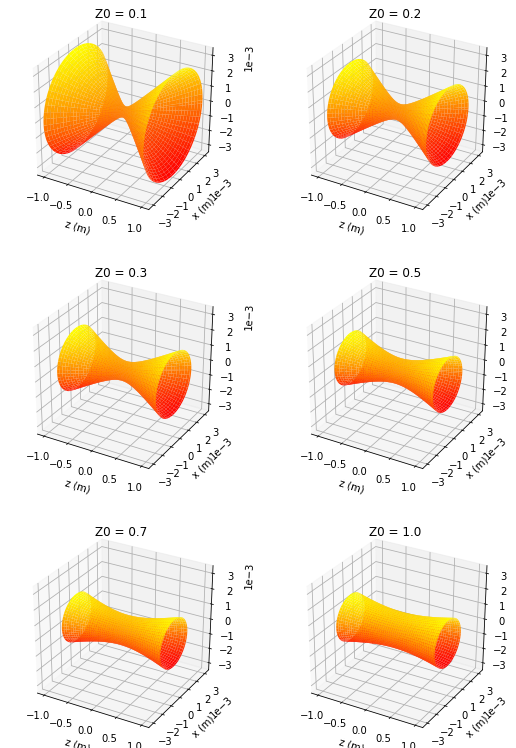
\includegraphics[scale=0.85]{images/chapter-3/Gaussian_beams_3d_plots}
	\caption{The Gaussian beams of $\lambda = 3.5 \mu m$ lasers with Rayleigh lengths of 0.1m, 0.2m, 0.3m, 0.5m, 0.7 and 1.0m are shown. As the Rayleigh lengths get larger, the waist becomes smaller at the focus and the beams spread out more quickly at distances away from the beam focus. The shape and spread of an ideal Gaussian beam is dependent on its beam waist or focus. Smaller waists results in faster divergences than.}
	\label{fig:Gaussian_beams_3d_plots}	
	\end{figure}

	This chapter introduces the Gaussian beam model, the most efficient model of the laser beam, in particular the $\text{TEM}_{00}$ mode. The Gaussian $TEM_{00}$ beam contains all the parameters necessary for describing the behavior of laser beams inside and outside a cavity. With a transition into lasers, the symmetry of the problem now calls for the utilization of cylindrical coordinates. The coordinates of the system are now $\rho$, $\phi$ and z instead of the usual x,y and z in Cartesian space. The variable $\rho$ is defined to be the radial distance from the z axis and $\phi$ is the angle relative to some reference direction, where z is still z. Either x or y could have been chosen to be "z", the reference axis. However, we designate z as our reference axis since it is the propagation axis. The relationship between x and y to $\rho$ and $\phi$ is $x=r\cos{(\phi)} \text{ and } y=r\sin{(\phi)}$ with $\rho^2 = x^2 +y^2$. 
	
	Our first detour is on the basis set of coordinate systems. There is some misconceptions that the different coordinate systems somehow produce different results because the work and final solutions look different. This not true and all notions that different coordinate systems producing different results should cease. The solutions of a problem will vary between using different coordinate systems to model a problem, however their results should always be equivalent. What differs is the variables or basis set that is being used to build a solution. For most readers, the big justification for choosing the correct coordinate should be the difference in the amount of paper space that is used to solve a problem. For example, a problem may rely on only 2 of the 3 available variables of an appropriately chosen coordinate system while requiring all 3 when using an inappropriate coordinates system. This is described visually by \autoref{fig:gaus_justification}. This is an intuitive way of describing the symmetry of a problem.
	
	In optics, the reference axis is chosen to be z since we already designate the propagation axis to be z. The angle $\phi$ is not a concern when dealing with the most fundamental $\text{TEM}_{00}$ Gaussian beam as it is $\phi$ independent. Here is the Gaussian beam with no development or proofs. 
	
	\begin{equation}
	\label {eq:Gaussian Beam}
	\vec{\textbf{E}}(\rho,z)=\vec{\textbf{E}}_\textbf{o} 
	\frac{\omega_{0}}{\omega(z)} 
	\exp\bigg[\dfrac{-\rho^2}{\omega^2(z)}\bigg] \exp{\left[ik_z z - i \arctan{\left(\frac{z}{z_0}\right)}\right]}\exp{\left[ik \dfrac{\rho^2}{2R(z)} \right]}
	\end{equation}
	
	A Gaussian laser beam is a beam of electromagnetic radiation with a Gaussian profile for its electric and magnetic field. All the predictable and desired properties of a laser beam are contained within the \autoref{eq:Gaussian Beam} except for some nonlinear effects. As this section progresses, the individual components of the Gaussian beam will be discussed to provide details on their properties and usage. Although the Gaussian beam equation looks daunting, it is simple enough to understand when its components are analyzed separately. 
	
	To avoid confusion, Gaussian beams are not parallel rays of radiation and the Gaussian beam model is only accurate to within the paraxial limit. The paraxial limit is a small angle approximation that assumes the beam is close to propagation axis. The paraxial limit proves to be a good assumption since the beams exist locally around the propagation axis. The Gaussian beam model can be thought of as a curved cylinder sitting along the propagation axis at the center. This is because the symmetry of the Gaussian beam model is cylindrical, hence our choice of cylindrical coordinates over Cartesian. These assumptions are made because real lasers beams are typically small and travel along an axis hence the "beam" part of laser beams. It can be a little confusing to think of lasers as pillars of light as opposed to straights lines or rays of light as they are made to be in less involved discussions of laser beams. Just accept that this is how lasers actually work. The following \autoref{fig:gaus_justification} should elaborate on the reasons for making these assumptions.

	\begin{figure} [!ht]
	\centering
	\def\svgwidth{\columnwidth}
	\resizebox{16cm}{!}{\imginput{images/gaus_justification.pdf_tex}}
	\caption{A cartoon of a Gaussian laser beam. Notice the cylindrical symmetry of the beam. X and y are replaced with the radial distances $\rho$ and the angle radial distances make with the reference direction $\phi$. However, this is a $\text{TEM}_{00}$ which has no $\phi$ dependence. Along the z axis, laser beams spread and diverge at distance away from the focus. Therefore, the Gaussian beam can be described using only 2 variables, z and $\rho$ as opposed to 3 in Cartesian coordinates. In short, the Gaussian beam $\text{TEM}_{00}$ should have the same phase and electric field no matter what angle of phi is used.} 
	\label{fig:gaus_justification}
	\end{figure}
			
	Why go through so much just to describe a laser beam when we can simply use ray optics? That is because ray optics is too weak of a model to describe the lasing system of a cavity. It also proves to be an insufficient model for aligning laser beams. However, one important topic from ray optics does carry over, the ABCD law. All the assumptions that were made about small angles allow a Gaussian beams to following the same set of transformations caused by optical elements acting on rays vectors. This is because nonlinear components are assumed to be non existent in the Gaussian beam model, making them negligible when "staying close" to the propagation axis. In practice, laser beams do carry nonlinear terms and effects but they are unpredictable and thus undesirable. This is why cleaning the beam is necessary. It is to get rid of nonlinear terms of the laser beam to keep it close to the predictable Gaussian beam model. 
	
	Before moving on to the sections of this chapter, it is not necessary to read the sections in any particular order. It would be best to read this chapter more than twice to understand the complexity and beauty of the Gaussian beam model of a laser beam. The equations are laid out in such a way for ease of referencing when performing calculations. This book will also sometimes use the terms Gaussian beam, Gaussian laser beam and laser beam interchangeably even though they technically refer to different things. 
%-------------------------------------------------------------------------------%
	\section{Gaussian Beam Parameters and Factors}
		\label{sec:Gaussian Beam Parameters and Factors}
		The following are the parameters that describe the Gaussian beams phase, amplitude, and shape. Despite looking complex, the Gaussian beam \autoref{eq:Gaussian Beam} can be broken down into components for simpler analysis. Keep in mind that the Gaussian beam is model that combines the planar and spherical wave models.
		
		\begin{equation}
			\label{eq:Gaussian Beam Parameters}
			\begin{split}
			\text{Guoy Phase: }& \quad \zeta = \exp\left(-i\tan^{-1}{\dfrac{z}{z_o}}\right) \\
			\text{Beam Waist Parameter: }& w_0 = \sqrt{\frac{\lambda z_0}{\pi}}\\
			\text{Beam Waist: } & w(z) = w_0 \sqrt{1+\left(\frac{z}{z_0}\right)^2}\\
			\text{Wavefront Curvature: } & R(z)=z\left[1+\left(\frac{z_0}{z}\right)^2 \right]
			\end{split}
		\end{equation}
		
		\noindent These are the basic parameters used to describe the shape and phase of the Gaussian beam. When characterizing a Gaussian beam, the location of its focus and waist parameter must be defined. An alternatively to having the waist defined is the Rayleigh length of the beam. They both define the shape of the Gaussian laser beams. The following identities are factors describing intensity, direction and phase of the Gaussian beam.
		
		\begin{equation}
		\label {eq:Gaussian Beam Factors}
		\begin{split}
		\text{Electric Field Factor: }& \vec{\textbf{E}}_\textbf{o} \frac{\omega_{0}}{\omega(z)}\exp\bigg[\dfrac{-\rho^2}{\omega^2(z)}\bigg]\\
		\text{Longitudinal Factor: }& \exp\bigg[ik_z z - i \tan^{-1} \bigg(\frac{z}{z_0} \bigg) \bigg]\\
		\text{Radial Phase Factor: }& \exp\bigg[ik \dfrac{\rho^2}{2R(z)}\bigg] \\
		\end{split}
		\end{equation}
		
		With the beam broken down into the electric field, longitudinal and radial phase factors, it should be clear the connection the Gaussian beam has with the planar and spherical wave model. The following sections will describe the characteristic of the Gaussian beam more deeply. This subsections just serves as a reference for the names of the identities, parameters and factors of the Gaussian beam.
		
	\section{Guoy Phase}
		\label{sec:Guoy Phase}
		The Guoy Phase is a property of Gaussian beam model that distinguishes it from a plane wave model, even when staying in the paraxial limit. After traveling some distance z, the Gaussian beam has a phase shift decrease of $\pi$ in comparison to the plane wave model. This phase shift parameter is important as it is one of the marks of transition of the planar to spherical properties of the Gaussian beam. . The importance of the Guoy phase has its roots in an uncertainty relationship. One way to think about it is that when the beam is focused, the photons are squished together into the focus and the longitudinal phase elongate as a result. As the beam propagates outward, the phases contract again due to the relaxation of having the photons so close together. This occurs because an uncertainty principle of k vectors and space \cite{}.  
		
	\section{Divergence and Spread}
		\label{sec:Divergence}
		The "center" of a Gaussian beam is at its thinnest location which is referred to as the waist or focus. The location of the focus is always given the origin of the frame as the beam is symmetric in both direction with respect to the focus. Gaussian beams have a natural spread characterized by their divergence that is relative to the waist or focus of the beam. This results in the spreading of the beam as the the Gaussian beam propagates in either direction of its propagation axis. This spreading of the beam ends up diluting the intensity of the beam as it propagate further away z=0, the location of the focus. The rate of the spreading is related to the size of the focus with smaller focuses resulting in faster spreading relative to beams with larger focuses. The two parameters describing the shape of the beam is the following pair of equations. 
		
		\begin{equation}
		\label{eq: Gaussian Beam Shape}
		\begin{split}
		\text{Beam Focus: }& w_0 = \sqrt{\frac{\lambda z_0}{\pi}}\\
		\text{Beam Waist: } & w(z) = w_0 \sqrt{1+\frac{z}{z_0}^2}\\
		\end{split}
		\end{equation}
		
		Technically, the beam waist is dependent on the focus, but the focus is given it's own variable since the beam focus is so important. If the focus is the origin then for $z=0$, $\omega(z)|_{z=0}=\omega_o$. Note that when aligning a real beam, the origin may not always be at the focus of the beam as there will be many recollimation. A real lasing system will have a long cascades of transformation resulting in many collimation of the beam many times.
		
		Mathematically, the gaussian beam is a paraboloidal wave with respect to z in the complex plane. This means that the beam is mathematically zero at $z=i z_o$ but this is along the imaginary axis and thus has no real physical meaning. This is an important fact used in the ABCD law for describing the transformation of the gaussian beam via thin lens and spherical mirrors.
		
		As the beam propagates away from the z axis, the beam waist \autoref{eq: Gaussian Beam Shape} can be approximated by the 
		beam waist at far distance approximation. Using this approximation allows the definition of the far field divergence half angle which is the the length of the waist  relative to the propagation axis at far distances. This approximation works because at far distances, the Gaussian beam is dominated by its spherical nature which essentially makes the beam a cone at far distances. The far half field divergence half angle is essentially half the angle of this cone at the tip. The cone shape of the Gaussian beam can be seen in \autoref{fig:Gaussian_beams_waists}
		
		\begin{equation}
		\begin{split}
		\text{Beam Waist at far distances: } & w(z) \approx w_0 z\\
		\text{Far field divergence half angle: } & \frac{w(z)}{z_0} = \theta_0 = \frac{\lambda}{\pi w_0}
		\end{split}
		\end{equation}
		
		\noindent The far field divergence half angle is not that important. Usually, the focus and shape of the waist is a more important description of the beam. This is especially true when performing laser spectroscopy as the intensity of the beam is highest at its waist.
		
		\begin{figure} 
		\centering
		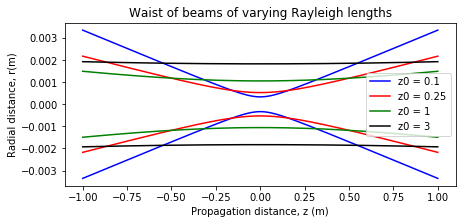
\includegraphics[scale=0.9]{images/chapter-3/Gaussian_beams_waists}
		\caption{Different Gaussian beams varying only by their Rayleigh length, ie the size of their focus. Smaller waists result in faster divergences as the beam propagates. with $z_0 = 1$ and $z_0 = 3$, we see that the mean is well collimated in comparison to $z_0 = 0.1$ and  $z_0 = 0.25$.  }
		\label{fig:Gaussian_beams_waists}	
		\end{figure}
	
	\section{Rayleigh Length}
		\label{sec:Rayleigh Length}
		The Rayleigh parameter is not expressed in the parameter set of \autoref{eq:Gaussian Beam Parameters} as it is inherent in the beam waist parameter. Including it would make the list of the parameter \autoref{eq:Gaussian Beam Parameters} redundant. However the Rayleigh length is still a useful way of describing the shape of a Gaussian beam as its length is more easily comprehendable by the human brain. Beam waists tend to be in the order of micro meters while Rayleigh lengths tend to be in the cm or meters. Either the beam waist parameter or the Rayleigh length is enough to describe the shape of a Gaussian beam as they are basically different ways of expressing the shape of a Gaussian beam. The Rayleigh length is also tbe preferable parameter because of its importance in the ABCD law in \autoref{sec:ABCD Law and Transformations}. The Rayleigh length is also much easier parameter to work with when creating computer simulations, plots and surfaces. In fact, all of these plots and calculation created in this book were done so with Rayleigh lengths in mind.
		
		\begin{equation}
		\label{eq:Rayleigh Length}
		\text{Rayleigh Length: } z_0 = \frac{\pi w_0^2}{\lambda}
		\end{equation}
		
		\noindent The Rayleigh length \autoref{eq:Rayleigh Length} is just the beam waist parameter rewritten for $z_0$ on the left hand side. That is why it is not include in the parameters \autoref{eq:Gaussian Beam Parameters}. From a scales perspective, the Rayleigh length is a larger parameter that is more easily understood by humans. Well collimated beams with low divergences can have of a couple centimeters or even a meter. The beam waist parameter is typically a tiny parameter that could be in the microns. And finally, a more systematic approach of comparing the shape of different beams is by comparing the waists at $z_0$ away from the focus. The waist of the beam has the special property of being equal to $w_0\sqrt{2}$
		
		\begin{figure} 
		\centering
		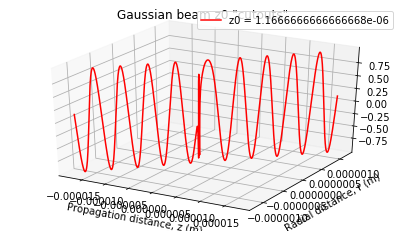
\includegraphics[scale=0.9]{images/chapter-3/Gaussian_beams_waists_at_z0}
		\caption{This figure shows cutouts of a Gaussian beam at z=z0. Larger well collimated beams have larger Rayleigh lengths or larger cutouts relative to Gaussian beams of smaller Rayleigh lengths.}
		\label{fig:Gaussian_beams_waists_at_z0}	
		\end{figure}
		
		The take away from this property is that it provides a more systematic mode of comparing beam shapes. From an intuitive perspective, it is enough to understand that smaller beam waists result in smaller Rayleigh lengths and faster divergence.
		
	\section{Polarization}
		\label{sec:Polarization}
		The direction of the electric field is always orthogonal to the direction of propagation which by convention is along the z axis. The electric field can point in either the x, y and a combination of both. This is known as the polarization of the beam. There can also be an associated phase shift for one of the component direction resulting in elliptically or circularly polarized light. Polarization is useful since it allows for the separation of a beam without affecting its frequency or trajectory. This can be see in figure \autoref{fig:ircease-setup} where the back reflection and input beam are separated by their orthogonal polarization at the polarized beam splitter.

		\begin{figure} 
			\centering
			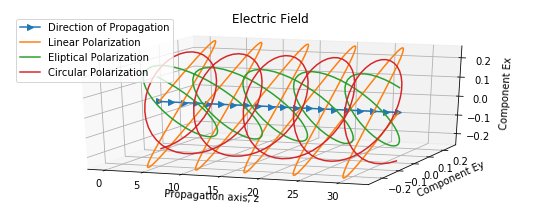
\includegraphics[scale=0.8]{images/chapter-3/Polarization_of_Electromagnetic_Radiation.png}
			\caption{The beam is traveling to the right, in the direction of the z axis. The transverse plane is the x and y plane which shows the transverse electric field. In the simulation are linear polarization, elliptical and circular polarization.}
			\label{fig:Polarization_of_Electromagnetic_Radiation.png}	
		\end{figure}
		
		The polarization properties of the Gaussian beam \autoref{eq:Gaussian Beam} are found in $\vec{E}_\textbf{o}$ vector. This vector represents the polarization of the beam and the intensity of the electric field at any given point and time. When this vector is broken down into its magnitude and unit vector form, we get the following identities.
		
		\begin{equation}
		\begin{split}
		\vec{E}_\textbf{o}  =& E_{o}			
		\left[\begin{matrix}
		a\hat{x}\\ b\hat{y}
		\end{matrix}\right]\\
		\text{Electric Field Intensity: }& E_{o} \\
		\text{Jones Vector: } &
		\left[\begin{matrix}
		a\hat{x}\\ b\hat{y}
		\end{matrix}\right]\\
		\end{split}
		\end{equation}
		
		\noindent The parameter of interest is the jones vector which is just the unit vector. Unit vectors contain the directional x and y components, the transverse planes, of the electric field. Remember that the direction of propagation is always assumed to be in the z direction. There are essentially 3 types of polarizations for a Gaussian beam, not including the their direction. These polarizations would be linear, elliptical and circular. Note that jones vector have some normalizing constant which is represented by $N$ constant.
		
		\begin{equation}
		\label{eq:jones vector}
		\begin{split}
		\text{Normalizing Factor: }& N \\
		\text{Linear: } & N
		\left[\begin{matrix}
		\cos{\theta} \\ \sin{\theta}
		\end{matrix}\right]\\
		\text{Ellipitcal: } & N
		\left[\begin{matrix}
		a \\ b+ic
		\end{matrix}\right]\\
		\text{Circular: } & N
		\left[\begin{matrix}
		1 \\ i
		\end{matrix}\right]
		\end{split}
		\end{equation}			
		
		Circularly polarizing has two directions, right and left just as how we have two hands. The difference is sign of one of the component. In \autoref{eq:jones vector}, the circular polarization is shown to be left hand. To obtain right handed circular polarization, the y component can be made negative. Circular and elliptical polarization result from having one of the components out of phase relative to the other component. We choose to phase shift the y component to keep the x component constant in all cases. Theoretically, only the linear and circular polarization of the electric field are of interest however, elliptical is discussed because circularly polarizing gone wrong results in elliptical polarizing. It is important to ensure that the correct thickness and material is chosen for the correct frequency when polarizing the Gaussian beam.
		
%-------------------------------------------------------------------------------%

	\section{Complex Electric Field}
		\label{sec:Complex Electric Field}
		This section provides details on the electric field and complex plane of the $\text{TEM}_{00}$ Gaussian laser beam and will set up for the following \autoref{sec:Intensity and Power} on the power and intensity of a Gaussian beam. This subsection also gently introduces the concepts and advantages of working within the complex plane for academic purposes. It should be noted that electric fields of electromagnetic radiation oscillate at frequencies greater than the gigahertz making them impossible to fully characterize. 
		
		Starting off with a quick explanation of on electric forces. Electric fields or forces are a type of force that act on charged bodies. For example, a proton and electron both exert electric fields that cause both particles to attract each other forming a hydrogen atom. The electric field of interest within optics is the oscillating electric fields found in electromagnetic radiation. Electromagnetic radiation have oscillating electric and magnetic fields. However, the magnetic field portion of EM radiation is largely ignored because magnetic interactions with matter are minuscule and ignorable. The magnetic field in electromagnetic radiation are typically only seen on paper when solving for boundary conditions of medias.  
		
		The electric field of the Gaussian beam \autoref{eq:Gaussian Beam} is its \textbf{complex} representation of the electric field, meaning that this electric has a real and an imaginary component. Electric fields in optics are often represented in their complex form since doing so simplifies many mathematical calculations by the pages. For example, taking series of derivatives of complex exponentials, $\exp^{-ikt} \rightarrow -ik\exp^{-ikt} \rightarrow {ik}^2 \exp^{-ikt}$, is  cleaner than taking derivatives of sinusoidal functions, $\sin{at} \rightarrow a\cos{at} \rightarrow -a^2\sin{at}$. Taking derivatives of exponentials is just a matter of bringing the constants down while keeping the same exponential function after each derivative whereas derivatives of sines an cosines involve changes into cosines an sines and tracking of signs an constants. We can interchange sines and cosines for complex exponentials since $\exp^{(it)}=\cos(t)+i \sin(t)$. Complex exponentials are actually vectors in the complex plane where the real axis contains real physical information of the sinusoid and the imaginary axis is used as a tool for "book keeping" the phase of our sinusoid which we can throw away when needed.
		
		Moving the electric field to a complex electric to work within the complex plane is seemingly difficult and abstract at first. However, doing so provides many benefits of simplifying the math manipulations when trying to derive physical results. For example, calculating the intensity of a Gaussian can beam can be done by throwing the phase components in \autoref{eq:Gaussian Beam Factors} and multiplying what is left with its complex conjugate. Doing this calculating with sin and cosine would results in at least half a page of work. Obtaining the real electric field again is a matter of throwing away the imaginary component. This is why it is called the imaginary component, because it holds no real physical information it can be ignored if need be. The overall idea is to perform operations that get rid of the imaginary component and leaving behind real components that provide real physical data.
		
		\begin{figure} 
		\centering
		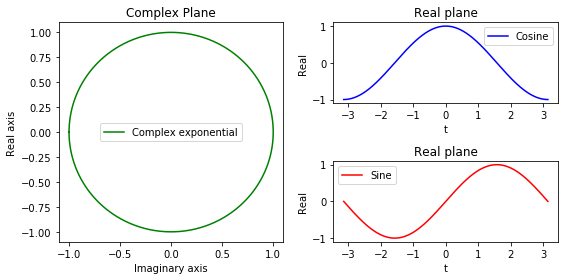
\includegraphics[scale=0.8]{images/chapter-3/Complex_exponential_sine_cosine.png}
		\caption{The larger plot on the left is a complex exponential plotted in the complex plane. The two plots on the right are cosine and sine in the real plane. Note that $\exp^{(it)}=\cos(t)+i \sin(t)$, which results in a circular plot in the complex plane. Note that in the circularly polarized electric field vector in \autoref{fig:Polarization_of_Electromagnetic_Radiation.png}, the x component of the electric field is $\cos(kz)$ while the y component is $\sin(kz)$.}
		\label{fig:Complex_exponential_sine_cosine.png}	
		\end{figure}
		
		The simple explanation for why moving to the complex plane works is that the imaginary component is used for "book keeping" the phase of the Gaussian beam or sinusoids. The mathematical relations are shown below in the electric field and intensity \autoref{eq:Intensity}.
		
		\begin{equation} 
			\vec{E}(\rho,z)=Re[\vec{\textbf{E}}(\rho,z)], \qquad
			\textit{I} \propto |\vec{\textbf{E}}(\rho,z)|^2=\vec{\textbf{E}}(\rho,z)\cdot \vec{\textbf{E}}^*(\rho,z)
			\label{eq:Intensity}
		\end{equation}
		
		Most of the content in this subsection would normally be put into the theoretical section, but introducing the basic concepts on complex before moving onto the intensity and power Gaussian beam seems to be a wise choice. The intensity profiles and power profiles are completely real and posses no phase components unlike the complex electric field of the Gaussian beam.

	\section{Gaussian Beam is a Mathematical Model}
		\label{sec:Gaussian Beam Model}
		With the complex notation taken care of, the intensity and power equation of a Gaussian laser beam can be analyzed. Mathematically, the Gaussian beam model is being moved from the complex plane, which consists of a real and imaginary axis, to only the real axis. This is important as the real axis contains physical information of our Gaussian beam model. Many students do not really understand that much of what is taught in classrooms are mathematical models since students are given the impression that these mathematical models are the physical systems. However, these mathematical models do accurately represent and characterize physical systems because when the models are built correctly with the correct conditions and assumptions. This is why so much effort is spent on studying math and how to apply math models to physical systems because studying them provide real physical information of that characterized physical systems. 
		
		The Gaussian beam \autoref{eq:Gaussian Beam} for example is a mathematical construct that exists in the complex plane. This book talks about Gaussian beams as if they are laser beams, but the Gaussian beam is just a solution to Maxwells equations and paraxial limit of the Laplace equation, which in term are all math equations that form a model. The Gaussian beam is being used to model a laser beam, but can be used in modeling other physical systems as well such as particle beams. From this model however, we are able to obtain physical results that characterize a physical laser beam. Using the Gaussian beam, we can model where the focus is or where the beam will be if we use an optical element to shape the beam. More generally, this is known as alignment of a lasing system which will be covered in the alignment section \autoref{asdf}. Most of what is known in physics starts off as assumptions and models that must prove to accurately model physical system before being accepted. This is why the Gaussian beam is used to model a laser beam and not the plane or spherical wave. Both the plane and spherical wave model are to simple to characterize a laser beam. Hopefully, this provides insight as to why theory and mathematical models are important to physics. The general idea is that the theory must be understood first before the experimental can fully be understood. In summary, the Gaussian beam is a mathematical model that characterizes a laser beam.
		
	\section{Intensity and Power}
		\label{sec:Intensity and Power}
		
		\begin{figure} 
		\centering
		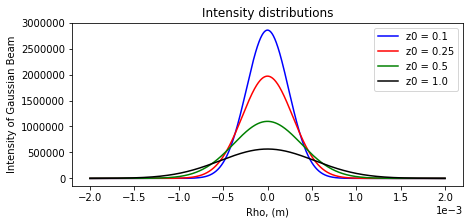
\includegraphics[scale=0.8]{images/chapter-3/Intensities_Distribution_beams.png}
		\caption{The intensity profiles of Gaussian beams are Gaussian in shape. The two intensity surface plots are normalized by having the same power output. The intensity distributions themselves are not normalized and should not be as intensity is related to density of the radiation. Smaller focuses result increases square fold increases of intensity.  }
		\label{fig:Intensities_Distribution_beams}
		\end{figure}
	
		From the Gaussian beam model of a laser beam, we can obtain the quantities of a Gaussian beam that characterizes the time average intensities and the total power of a laser beam. The intensity and power of a laser beam will allow us to create a Gaussian beam model that provides information about th laser beam. Trying to use a plane wave or spherical wave model will result in failure as they individual cannot characterize the beam at its focus and far from its focus.  In the infrared region of electromagnetic radiation, being able to detect power and intensity of a laser beam is crucial as infrared is invisible to the human eye hence we must rely on detectors to be sure of their presence.
		
		\begin{equation}
		\label{eq:Intensity and power of Gaussian beam}
		\begin{split}
		\text{Intensity: }& I(\rho, z) = I_0 \left[ \frac{w_0}{w(z)} \right] ^2 \exp{\left[ -\frac{2r^2}{w^2(z)}\right]}\\
		\text{Power: } & P = \frac{I_0}{2} \left(\pi w_0^2\right) \\
		\end{split}
		\end{equation}
		
		The intensity and power \autoref{eq:Intensity and power of Gaussian beam}s of the Gaussian laser beam are real and measurable. Being able to measure both the intensity, power and shape of beam provides critical information for alignment such as where the focus of the beam is located and the shape of its waist or focus. At minimum, two measurements of the beams power or intensity must be made in order to characterize the laser beam. More measurements is always nice as more data can be used to constrain its Gaussian beam model. The electric field is not included in \autoref{eq:Intensity and power of Gaussian beam} because measuring the frequency of an electromagnetic wave is impossible as current detection systems are not fast enough to keep up with the gigahertz frequencies. What is measured instead is the time average of the intensity or power of the beam. 
		
		\begin{figure} 
		\centering
		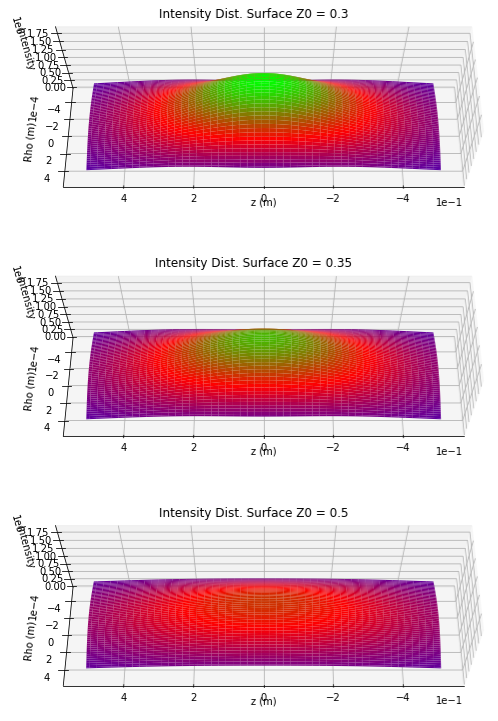
\includegraphics[scale=0.85]{images/chapter-3/Intensities_Distribution_3ds.png}
		\caption{The 2 surfaces shown are the intensity distribution surfaces of Gaussian beam model of the infrared wavelength of 3.5nm with Rayleigh lengths of 0.1m and 0.15m. A large radial distances away from the propagation axis, a dip in the intensity can be seen at around the focus. This is because most of the intensity of the beam is located at around the focus, z=0, of the laser. As the beam propagates away from the focus, the beam begins to diverge and becomes larger radially.}
		\label{fig:Intensities_Distribution_3d}	
		\end{figure}
		
		From the surface plots of intensity in \autoref{fig:Intensities_Distribution_3d}, the shape of a Gaussian laser beam can be around the base of the plot. One can kind of think of taking measurements of the laser beam to figure out the shape and properties of the base, ie its Rayleigh length, so that a Gaussian beam model can be used to predict the characteristic of the beam at other such as the location of its focus. Very critical concept when aligning infrared laser beam.
		
		
%-------------------------------------------------------------------------------%
	\section{K vector}
		\label{sec:K vector}
		The k vector is given, by eq(\autoref{eq:kvector}), contains information about the wavelength(frequency) and direction of propagation of the ray or wave or in particular, the Gaussian beam.
		
		\begin{equation} 
		\label{eq:kvector}
		\vec{k} = \langle k_x,k_y,k_z \rangle, \qquad |\vec{k}|=\dfrac{2\pi}{\lambda}
		\end{equation} 
		
		\noindent The k vector is more generally known as the spatial angular frequency of a wave and characterizes the rate that a wave oscillates within space. Basically, the wavelength is th distance that a wave must propagate in order to complete 1 cycle. Longer wavelengths result in smaller k vectors There is really not much else to say about k vectors.
		
		\begin{figure} [!ht]
		\centering
		\def\svgwidth{\columnwidth}
		\resizebox{16cm}{!}{\imginput{images/gaus-beam-prop.pdf_tex}}
		\caption{In this figure, the Gaussian Beam's properties are shown at various z: z=0 and the Rayleigh lengths to help visualize the Gaussian Beam.
		\newline
		{\bfseries (A)} The Gausian intensity distribution along transverse planes at various z values
		\newline
		{\bfseries (B)} Intensity distribution along a section in the transverse plane at the focus and  $z=z_\alpha$.
		\newline
		{\bfseries (C)} A plot of the waist size of a Gaussian beam and constant phase of the electric field to illustrate the plane wave and spherical wave limits in the curvature of a beam
		\newline
		{\bfseries (D)} Plot of the radius of curvature, flat wavefronts have infinite curvature while spherical wave have linearly increasing curvature} 
		\label{fig:gaus-beam-prop}
		\end{figure}	

%-------------------------------------------------------------------------------%
		
%-------------------------------------------------------------------------------%
	\section{Wavefront and Curvature}
		\label{sec:Wavefront and Curvature}
		When describing electromagnetic waves, the two classic models are the plane and spherical waves. However, the wave model of importance when modeling lasers is the Gaussian beam. The Gaussian beam model which can be thought of as a hybrid of the plane and spherical wave models. The plane and spherical waves differ by their source, nature of propagation and shape of their wavefronts. Wavefronts are the locations of the beam where the phase is constant, such as phases of 0 or $\pi$. The parameter used to describe the wavefront at a given location is curvature \autoref{eq:curvature} and its inverse, radius of curvature.
		
		\begin{equation}
		\label{eq:curvature}
		\kappa = \frac{1}{R}
		\end{equation}
		\noindent In the spherical wave and Gaussian beam model, the curvature of the wavefronts are dependent on the distance from the point source and focus respectively. From the spherical wave in \autoref{fig:wavefront}, the circular slice of the wavefronts from the point source get larger as the spherical propagates outwards. The radius of these spherical wavefronts are R, the radius of curvature. Wavefronts linearly increase as the wave moves radially outward. The Gaussian beam follows the same trend as the spherical wave how ever, the more technical definition of curvature must be used in order to describe the Gaussian beam as the wave fronts are not exactly circular except for at far distances from the focus. Curvature is the is defined as the local tendency of a surface or plane to curve hence the nonlinear R(z) \autoref{eq:Gaussian Beam Parameters} of a Gaussian beam. 
		\begin{equation}
		\label{eq:phase fronts of planes, spherical and Gaussian}
		\begin{split}
		\text{Plane waves: }& \exp{ \left[-i k_z z \right]} \\
		\text{Spherical waves: }& \frac{1}{R}\exp{\left[-ikR\right]} \approx \frac{1}{R}\exp{\left[-i\left(kz +\frac{r^2}{2R}\right)\right]} \\
		\text{Gaussian beam: }& \exp{\left[ik_z z - i\arctan{\left(\frac{z}{z_0}\right)}\right]}
		\exp{\left[ik \dfrac{\rho^2}{2R(z)} \right]}
		\end{split}
		\end{equation}
		
		\begin{figure} 
		\centering
		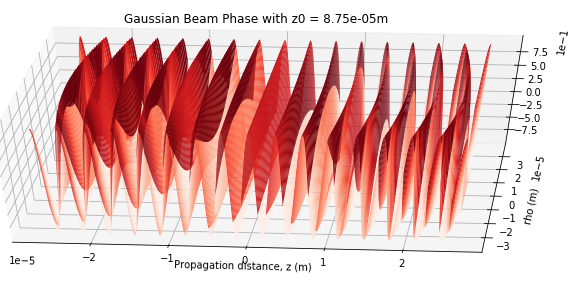
\includegraphics[scale=0.8]{images/chapter-3/Gaussian_beam_phases1}
		\caption{This is plot of the phase in the real axis of the Gaussian beam wave. The wavelength is 3500nm with a Rayleigh length of 25 times the wavelength. Within 1 wavelength of its propagation distance, the Gaussian beam appears to be planar}
		\label{fig:Gaussian_beam_phase}
		\end{figure}
		By nature, the shape of the wavefronts are planar or spherical, hence the names of the wave models. Likewise, the Gaussian beam model has Gaussian like wavefronts. \autoref{eq:phase fronts of planes, spherical and Gaussian} shows the phase components of the plane wave, spherical wave and Gaussian beam. The \autoref{eq:phase fronts of planes, spherical and Gaussian} contains the phase component of the 3 wave models. The phase component of the Gaussian beam appears daunting in comparison to the plane and spherical wave, but the Gaussian beam can be simplified by analyzing the individual components like the all other components of the Gaussian beam model.
		
		For plane waves, phase fronts occur along a transverse plane as shown in \autoref{fig:wavefront}, along a straight line for all x values at a fixed z value. By nature, plane waves always propagate uniformly in a single direction and have wavefronts perpendicular to their axis of propagation. The wavefronts could also be constant along the y axis or a combination of the y and x axis. The surfaces produced by plane waves have flat wavefronts, no curvature or infinite radius of curvatures. 
		
		For spherical waves, the wavefronts are spherical with linearly increasing radius as the wave propagates outward from the source. Unlike the planewave model, spherical waves propagate outwards from a point source. The wavefronts of spherical waves are finite and have radius R relative to the point source.
		
		The Gaussian beam is a mix of a plane wave and spherical wave making it a hybrid of the two models. From \autoref{eq:Gaussian beam phase}, we can see that the phase factor of the Gaussian beam contains a plane wave and spherical wave component . The Guoy phase mentioned in the Guoy Phase \autoref{sec:Guoy Phase} provides information on when the beam transitions from plane wave like to spherical wave like. This transition occurs at its Rayleigh length, $z = \pm z_0$. As the Gaussian beam propagates along the z axis, the beam waist gets larger along the transverse planes meaning the spherical component begins to dominate at large $\rho$. This can be seen in \autoref{fig:Gaussian_beams_waists} at distances far from $z = 0$.
		
		\begin{equation}
			\label{eq:Gaussian beam phase}
			\begin{split}
			\text{Gaussian beam phase: }& \exp{\left[ik_z z - i \arctan{\left(\frac{z}{z_0}\right)}\right]}
			\exp{\left[ik \dfrac{\rho^2}{2R(z)} \right]}\\
			\text{Plane wave component: }& \exp{ \left[ i k_z z \right]} \\
			\text{Spherical wave component: }& \exp{\left[ik \dfrac{\rho^2}{2R(z)} \right]} \\
			\text{Guoy Phase: } & \exp{\left[ - i \arctan{\left(\frac{z}{z_0}\right)}\right]} \\
			\end{split}
		\end{equation}
		
		\begin{figure} [!ht]
			\centering
			\def\svgwidth{\columnwidth}
			\resizebox{16cm}{!}{\imginput{images/wavefront.pdf_tex}}
			\caption{To illustrate the curvature of the wavefronts of the plane, spherical, and Gaussian models} 
			\label{fig:wavefront}
		\end{figure}	
		
		The Gaussian beam can be approximated by a plane wave close to the focus of the beam. For beams that are well collimated, the beam must travel a distance, $z=z_0$, farther before the beam become more spherical like. This is because a well collimated beam has a very low spread and larger Rayleigh length. Meaning that as the beam propagates, the waist of the beam increases slowly relative to the beam waist. The curvature of the phase fronts have become more spherical like as the by the Radial Phase Factor: $ \exp\bigg[ik \dfrac{\rho^2}{2R(z)}\bigg]$ in equation \autoref{eq:Gaussian Beam Factors}
		
		\begin{figure} 
		\centering
		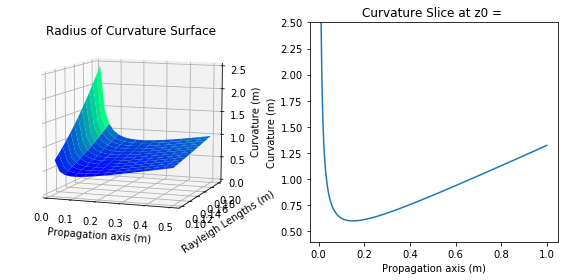
\includegraphics[scale=0.8]{images/chapter-3/Radius_of_curvature_3d.png}
		\caption{The beam is traveling to the right, in the direction of the z axis. The transverse plane is the x and y plane which shows the transverse electric field. In the simulation are linear polarization, elliptical and circular polarization.}
		\label{fig:Radius_of_curvature_3d.png}
		\end{figure}
	
		
	\section{ABCD Law and Cascade Systems}
		\label{sec:ABCD Law and Transformations}
		
		All that is really necessary from this section is that ABCD law works in describing transformations of Gaussian beams and the mathematical knowledge on how to work with its ABCD law's two equation. A warning that a bit of knowledge of complex variables is necessary to understand the math manipulation. The complex numbers \autoref{} will provide details on how to manipulate the the arithmetic to obtain the desired form of the q parameter. Here are the fundamental set of equations of the ABCD law. 
		
		\begin{equation}
		\label{Q parameter and ABCD law}
		\begin{split}
		\text{The q parameter: } & q(z) = z +iz_0 \\
		\text{Inverse q parameter: }& \frac{1}{q(z)}=\frac{1}{R(z)}+\frac{i\lambda}{\pi w^2(z)}\\
		\text{ABCD law: } & q_2=\frac{Aq_1 + B}{Cq_1 + D} \\
		\text{ABCD law: } & \dfrac{1}{q_2} = \frac{C + \dfrac{D}{q_1}}{A+\dfrac{B}{q_1}}
		\end{split}
		\end{equation}
		
		To start things off, the q parameter, $q = z +iz_0$, in \autoref{Q parameter and ABCD law} is a parameter that contains a Gaussian beam's location and shape. The location of the focus is inherent in its real component and its Rayleigh length in its imaginary component. In this section, a transformation matrix is a matrix that maps a 2 dimensional vector into another 2  dimensional vector. In application to ray optics, optical elements transform rays of light by changing their direction and angle. Mathematically, optical element are represented by transformation matrices and ray vectors are defined to be a 2 dimensional vector. The first element of a ray vector is defined to be the direction perpendicular to the defined reference axis. The second element is defined to be the angle that the ray makes relative to defined reference axis. In ray optics, the transformation matrices maps the ray vector to its transformed vector. A short introduction is being made on ray optics to ensure that the readers understand that the ABCD law does not follow the matrix and vector multiplication that is used in ray optics, but instead follows the ABCD law. Technically, there is a relation. However, to avoid having readers believe the the location of the focus and Rayleigh lengths are different elements in a vector, we stress that only the ABCD law must be used when describing transformation of Gaussian beams by optical element.
		
		There are optical elements that propagate, reflect, and refract electromagnetic radiation. A list of optical elements and their transformation matrices are given in \autoref{eq:transformation matrices}. Although these ray matrices are derived from ray optics, these transformation matrices of optical elements also transform the describe q parameter of a Gaussian beam. The ABCD law of \autoref{Q parameter and ABCD law} shows the transformed $q_2$ from the operation matrix operating on $q_1$ parameter. This transformation of a q parameter of a Gaussian beam is given in describe in two math equation in the ABCD law of \autoref{Q parameter and ABCD law}. Both math equations are actually equivalent but given in different forms. To get the inverse form, manipulation of the complex number is required to get rid of the imaginary component in denominator. This is done by multiplying the numerator and denominator by the complex conjugate of the q parameter, $q^*=z-iz_0$.
		
		\noindent The following are the transformation matrices of commonly used optical elements. The important idea to remember is that the following optical elements can change the location of the focus and the shape of the Gaussian beam. The following section on thin lens and mirrors will provide the basics on how optical elements transform Gaussian beams and how to apply the ABCD.
		\begin{equation}
		\label{eq:M}
		\text{Transformation Matrix: } \textbf{M} = \begin{bmatrix}
		A & B \\
		C & D  
		\end{bmatrix}
		\end{equation}
		
		asdf
		\begin{equation}
		\label{eq:transformation matrices}
		\begin{split}
		\text{Spherical Mirror: }& \textbf{M} =
		\begin{bmatrix}
		1 & 0 \\
		\dfrac{2}{R} & 1  
		\end{bmatrix} \\
		\text{Propagation distance: }& \textbf{M} =
		\begin{bmatrix}
		1 & d \\
		0 & 1  
		\end{bmatrix}\\
		\text{Thin Lens: } & \textbf{M} = 
		\begin{bmatrix}
		1 & 0 \\
		-\dfrac{1}{f} & 1  
		\end{bmatrix}\\
		\text{Planar Mirror: } & \textbf{M} = 
		\begin{bmatrix}
		1 & 0 \\
		0 & 1  
		\end{bmatrix} \\
		\text{Planar refractive index: } & \textbf{M} = 
		\begin{bmatrix}
		1 & 0 \\
		0 & \dfrac{n_1}{n_2}  
		\end{bmatrix} \\
		\text{Spherical refractive index: } & \textbf{M} = 
		\begin{bmatrix}
		1 & 0 \\
		-\dfrac{(n_2-n_1)}{n_2R} & \dfrac{n_1}{n_2}  
		\end{bmatrix} \\
		\end{split}
		\end{equation}
		
		\noindent A cascade matrix is the resulting matrix from a series of transformation from optical elements and propagation. Cascade matrices are ordered from right to left, the order that the matrices operate on the Gaussian beam's q parameter. Typically, Gaussian beams are drawn to propagate from left to right. Just remember that the two are in the opposite direction of each other as it is a very common mistake to order the transformation matrices the same way Gaussian beams are drawn. The most important optical systems this book will discuss are the cavity and the double lens system. The following \autoref{eq:Cascade Matrices} and \autoref{eq:Cavity cascade matrix} serve as demonstrations on how to create cascade matrices.
		
		\begin{equation}
		\label{eq:Cascade Matrices}
		\begin{split}
		\text{Cascade Matrix: } & \textbf{M} = 		\begin{bmatrix}
		A_c & B_c \\
		C_c & D_c  
		\end{bmatrix} 
		=
		\begin{bmatrix}
		A_1 & B_1 \\
		C_1 & D_1  
		\end{bmatrix}
		\begin{bmatrix}
		A_2 & B_2 \\
		C_2 & D_2  
		\end{bmatrix}
		\begin{bmatrix}
		A_3 & B_3 \\
		C_3 & D_3  
		\end{bmatrix}
		\begin{bmatrix}
		A_4 & B_4 \\
		C_4 & D_4  
		\end{bmatrix}
		\end{split}
		\end{equation}
		
		An optical cavity is type of resonator that stores optical energy. It consists of 2 reflecting surface that can be thought of as bouncing a Gaussian laser beam back and forth. A cartoon example of an optical cavity can be found in \autoref{fig:feb-per-cav}. The \autoref{sec:Optical Cavity and Resonance Properties} on optical cavity will explain in depth how optical resonators work. For now, we just introduce the cavity matrix of spherical resonator as an example to work with for developing cascade matrices. Optical cavities are a type of resonator that store optical energy by the use of 2 reflective surfaces. Symmetric confocal optical ]cavities that consists of two spherical reflecting mirrors facing each other. This type of cavity is explored since it possesses the property of having the focus of a resonating Gaussian beam somewhere within the cavity. This is important for spectroscopy since we want to use the point of absorption to have the highest intensity. Remember that from Beer-Lambert's law, the rate of absorption is relative the intensity of the beam with higher intensities resulting in higher absorptions leading to stronger signals. From \autoref{fig:Intensities_Distribution_3d}, the highest intensity of a beam is located at its focus, z=0, with lower Rayleigh lengths producing much higher intensity focuses. The Gaussian beam that resonates within a cavity can be found by finding the determinant of its cascade matrix. The cascade matrix of a cavity is referred to as the Cavity Matrix. Note that the author was the first person to solve this problem.
		
		\begin{figure} [!ht]
		\centering
		\def\svgwidth{\columnwidth}
		\resizebox{150mm}{!}{\imginput{images/ABCD_cavity.pdf_tex}}
		\caption{At starting point \textbf{A}, the beam propagates to the right to mirror 2 at point \textbf{B}. After reflecting from mirror 2, the laser propagates a distance $L_{cav}$ the right towards point A after which we make a round trip. The order of these transformation is propagation a distance $L_{cav}$, then reflection off of mirror 2, propagation a distance -$L_{cav}$ and finally reflection off of mirror 1.}
		\label{fig:ABCD_cavity}
		\end{figure}
		
		\begin{equation}
		\label{eq:Cavity cascade matrix}
		\begin{split}
		\text{Cavity Matrix: }  \textbf{M} = & \textbf{M}_{\text{S.mirror1}}\textbf{M}_{\text{-L}} \textbf{M}_{\text{S.mirror2}} \textbf{M}_{\text{L}} =
		\begin{bmatrix} A_c & B_c \\ C_c & D_c   \end{bmatrix}\\ = & \begin{bmatrix} 1 & 0 \\ \dfrac{2}{R_1} & 1 \end{bmatrix} \begin{bmatrix} 1 & -L \\ 0 & 1 \end{bmatrix} \begin{bmatrix} 1 & 0 \\ -\dfrac{2}{R_2} & 1 \end{bmatrix} \begin{bmatrix} 1 & L \\ 0 & 1 \end{bmatrix} \\ 
		\text{Cavity Matrix: }  
		= & \frac{1}{R_2}\begin{bmatrix} 2L +R_2 & 2L^2 \\ 2\left( \dfrac{2L-R_1+R_2}{R_1}\right) & \dfrac{4L^2-2R_1L+R_2R_1}{R_1} 1 \end{bmatrix}\\
		\text{Cavity Polynomial: } = & \lambda^2 -\Tr(\textbf{M}) +\det(\textbf{M}) = 0 \\ 
		\text{Trace of M: }\Tr(\textbf{M}) = & \dfrac{A+D}{2} = \dfrac{2L+R_2 + 4L^2  - 2R_1L  + R_1R_2}{2} \\
		\text{Determinant of M: } \det(\textbf{M}) = & 1 \\
		\text{Eigen Vectors: } = & \left[\textbf{M}-\lambda_{\pm} \textbf{I}\right]v_{\pm} = 0 \\
		\end{split}
		\end{equation}
		
		\noindent The eigen values of a matrix are $\lambda_+$ and $\lambda_-$. They are obtained by solving the cavity polynomial of \autoref{eq:Cavity cascade matrix}. From the eigen values, the eigen vectors of the cavity matrix are obtained by taking difference of the matrix and the $\lambda_{\pm} \textbf{I}$ times the eigen vector and solving for when it is zero. The resulting eigenvectors of the cavity polynomial of \autoref{eq:Cavity cascade matrix} forms one of the resonating conditions for a cavity. Using this method will obtain the specific polarity required for a resonating beam.
		
		\begin{equation}
		\label{eq:double lens cascade matrix}
		\begin{split}
		\text{Cavity Matrix: }  \textbf{M} = & \textbf{M}_{\text{lens1}}\textbf{M}_{\text{distance}} \textbf{M}_{\text{lens2}} \\
		= & \begin{bmatrix} 1 & 0 \\ -\dfrac{1}{f_2} & 1 \end{bmatrix} \begin{bmatrix} 1 & d \\ 0 & 1 \end{bmatrix} \begin{bmatrix} 1 & 0 \\ -\dfrac{1}{f_1} & 1 \end{bmatrix} \\ \text{Cavity Matrix: }  Z= & \begin{bmatrix} 1-\dfrac{d}{f_1} & d \\ -\dfrac{f_2+f_1-d}{f_2f_1} & 1-\dfrac{d}{f_2} \end{bmatrix}
		\end{split}
		\end{equation}
		
	\section{Gaussian Modes}
		\label{sec:Gaussian Modes}
		
		%	\begin{figure} 
		%		\centering
		%		\includegraphics[scale=0.9]{images/GaussianMode.png}
		%		\caption{\cite{hermite} \cite{Laguerre} The $TEM_{00}$ mode along with the other higher order Hermite modes.}
		%		\label{fig:Hermite-gaussian}	
		%	\end{figure}
		
		There are many different Gaussian modes that can resonate within a cavity, but the $TEM_{00}$ mode is the simplest and lowest order Gaussian beam solution to the Helmholtz equation. Higher order modes possess nodes that can be axial and radial nodes as in the cases for Hermite and Laguerre Gaussian modes. The Hermite and Laguerre modes are denoted by $TEM_{xy}$ and $TEM_{pl}$ with the x,y variables representing Cartesian coordinates and p,l representing cylindrical coordinates. Analogous to the electron orbitals, the higher the number of nodes, the higher the energy of the mode and lower the stability of the mode. Keep in mind that the complexity of the electric field increases as modes increases in order. The complex electric field of the $TEM_{00}$ mode is simplest which has the effect of coupling the greatest amount of energy into the intensity of the beam. The intensity of the beam is important as that is what we are measuring in laser absorption spectroscopy. Higher order modes just contain \autoref{eq:Gaussian Beam} multiplied by some linear combination of the polynomial basis sets, such as Hermite and Laguerre in combination with modification to the Guoy Phase. The following are the electric field and Guoy phase of a Gaussian beam.
%-------------------------------------------------------------------------------%
\chapter{Important Optical Systems}
	\label{chp:Important Optical Systems}
	This section requires all of the contents of the Gaussian beam \autoref{chp:Gaussian Beam} to be understood. This chapter takes all of the theory from the Gaussian beam model and apply them to practice and application of the Gaussian laser beam. This chapter will discuss double lens system for beam focusing and shaping, the optical resonator or better known as a cavity, and so forth should we get to it. This section is very complex and heavily dependent on the results and properties discussed in the Gaussian beam \autoref{chp:Gaussian Beam}. From the wavefronts, ABCD law, intensity profile, electric fields, polarization and so forth, accurate mathematical models of cavity will be produced. As stated, these math models help us characterize and predict these physical systems. Essentially, we are exploring a problem with the lights on as opposed to turning of the lights and just trying things out. 
	
	To keep the cavity discussion simple, we will only focus on the development of the symmetric confocal cavity or spherical cavity since this is the best cavity for all laser absorption system. The cascade matrix of the spherical cavity will also be brought over into the a discussion here to generalize the stability of a cavity.
	
	\section{Thin Lens and Spherical Mirrors}
		\label{sec:Thin Lens and Spherical Mirrors}
		Here quick statements and properties of converging lens and mirrors are discussed so that the interaction of the gaussian beam and mirrors or lens are understood, as well as their connection to ray optics. From ray optics, the transformation of planewave and spherical wave limits upon interaction of spherical lens are derived where the ABCD law expands upon these results to describe more practical and realistic Gaussian beam.
		
		A common optical element everyone has seen is a magnifying glass which contains a singular large converging lens. 
		This lens can be used to magnify or reimage spherical point emitters from nearby objects or focus plane wave radiation from the sun to the focal point depending on how far away the lens is examined from.
		The focal point of a lens or mirror, in the plane wave limit, is the transverse plane where plane waves are focused to. 
		Input beams with small tilt angles are slight shifted up or down depending on the sign of the tilt, a very useful property where an iris can be placed to clean the Gaussian beam. 
		The general relation between the focus of the input wave and output wave is given below in \autoref{focal} where the 0 is at the location of the optical element. 
		For a spherical element, the magnitude of the focal length is half the radius of the spherical element, $f=R_{element}/2$ and is positive for converging lenses and negative for diverging lenses.
		
		\begin{equation}\label{focal}
			\frac{1}{f}=\frac{1}{z_{output}}-\frac{1}{z_{input}}
		\end{equation}

		\begin{figure} [!ht]
			\centering
			\def\svgwidth{\columnwidth}
			\resizebox{150mm}{!}{\imginput{images/lens-reimage-focus.pdf_tex}}
			\caption{
				This figure illustrates the connection between the simple ray optics properties of lenses and ABCD gaussian beam model.
				\newline 
				\textbf{A}) Here the lens maps the point emitting spherical waves at $z=-z_o$ to $z=z_1$. There is a flip of the image at $z_1$ relative to $z_0$.
				\newline
				\textbf{B})For a gaussian beam at the spherical limit, a lens refocuses a beam at $-z_o$ to $z_1$
				\newline
				\textbf{C}) Plane waves are focused to the focal point. Where the plane is mapped to on the focal point depends on the angle of the beam relative to the lens axis.
				\newline
				\textbf{D}) For a Gaussian beam where the lens is located at the focus, very similarly to the plane wave limit, the beam is focused at the focal plane. Any beam coming in at a angle will be mapped above or below}
			\label{fig:lens-reimage-focus}
		\end{figure}
		
		Since the gaussian beam is a mix of plane and spherical wave model, the slightly more advanced ABCD law is required where the matrix transformation acts on the zero of the complex paraboloidal wave in the complex plane of the propagation axis, z.
		The location of the zero of the paraboloid is at $z=-iz_o$ which is a purely imaginary number thus has no physical interpretation, consistent with the fact that the size of a beam is always finite.
		Any transformation at the zero location in the complex plane though carries over to the real axis where the beam physically exists.
		Visually, the result of the transformation is that the wavefront curvature of the output beam is approximately matched to the curvature of the input surface.
		This is supported by the eikonal equation from ray optics \cite{SalehTeichs}.
		Illustrations can be shown below in \autoref{fig:Mirrors}. 
		The use of these results will be illustrated in mode matching and resonating beams in \autoref{sec:Optical Cavity and Resonance Properties} and \autoref{sec:Aligning the IR Cavity}.
		
		\begin{figure} [!ht]
			\centering
			\def\svgwidth{\columnwidth}
			\resizebox{160mm}{!}{\imginput{images/Mirrors.pdf_tex}}
			\caption{\cite{SalehTeichs} Mirrors are mostly reflecting at the wavelength of interest.
				a) Planar mirror with $R=\infty$ \quad b) Radius of the coated surface is some value $R_o$ \quad c) Here the focus of the beam is exactly at the focal point of the mirror which is half the radius of the surface.
			}
			\label{fig:Mirrors}
		\end{figure}	
		
		Mirrors have almost the exact same transformation properties of thin lenses except now the transformed beam travels in the reverse direction, ie the k vector is transformed. \autoref{fig:Mirrors} shows how mirrors reflect Gaussian beams where the dash lines represents the beam if it was transmitted like a lens.
		The transmitting and reflectivity property of mirrors and lenses are described by reflectivity coefficient. 
		Highly reflecting materials are classified as mirrors, they usually consist of metals or thin coatings. 
		Lens are specialized pieces of glass that are transparent to certain range of frequencies.
		Assuming minimal loses of energy to the material, the percentage of radiation that is reflected and transmitted is approximately 1. 
		The reflectivity coefficient of an optical element is $r$ and the reflectiveness of the lens is $\mathcal{R}=|r|^2$. The percentage of light reflected is given by R though and thus must be completely real.
		
		\begin{equation}\label{reflectivity}
			|r|^2+|t|^2=1, \quad |r|^2=\mathcal{R}, \quad |t|^2=\mathcal{T}, \quad \mathcal{R}+\mathcal{T}=1
		\end{equation}
		
		Note reflectivity and transmission coefficient, little r and little t, can be complex numbers resulting in phase shifts of the transformed wave. More info about ray optics and beam optics can be found in ref\cite{SalehTeichs} and \cite{steck} in their respective chapters.
		
%-------------------------------------------------------------------------------%
		\subsection{Double Lens System}
			\label{subsec:Double Lens System}
			A double lens system is exactly what a sounds like, it consists of a pair of two lenses that can be used to resize, recollimate, and or relocate the focus of a beam. Reshaping and moving the focus of a beam is important for efficient coupling of power into a cavity.
			
			\begin{figure} [!ht]
				\centering
				\def\svgwidth{\columnwidth}
				\resizebox{160mm}{!}{\imginput{images/double-lens-system.pdf_tex}}
				\caption{The important concept is that the focus and size of beam can be modified by two lens by varying the distance between the two lenses. For this plano convex lens system in particular, as the second lense is moved further away, the wider and closer the focus is to the lens.
				}
				\label{fig:double-lens-system}
			\end{figure}
%-------------------------------------------------------------------------------%
%-------------------------------------------------------------------------------%
	\section{Optical Cavity and Resonance Properties}
		\label{sec:Optical Cavity and Resonance Properties}
		An optical cavity is a type of resonator that uses mirrors with high reflectivity to store optical energy of specific frequencies. Cavities are typically used for reducing the bandwidth and/or collimation of an input Gaussian beams. The Fabry Perot is the simplest stable type of cavity for resonating Gaussian Beams consisting of 2 planar mirrors with resonant beam being plane waves. Optical power build up for frequencies that form a standing wave after 1 round trip within the cavity.The frequencies that satisfy this periodic condition. 
		
		\begin{equation}\label{eq:resonantfreq}
			\nu_q=\dfrac{cq}{2L_{eff}}, \qquad \tilde{\nu}_q=\dfrac{q}{2L_{eff}}
		\end{equation}
		
		The spacing between frequencies and wavelengths that satisfy this condition is know as the free spectral range.
		
		\begin{equation}\label{eq:FSR}
			\nu_{fsr}=\dfrac{c}{2L_{eff}}, \qquad \tilde{\nu}_{fsr}=\dfrac{1}{2L_{eff}}
		\end{equation}	
		
		If the resonant condition is not met, the radiation will interfere deconstructively with itself, similar to a Michelson interferometer, and exit back out through the input mirror.			
		
		\begin{figure} 
			\centering
			\def\svgwidth{\columnwidth}
			\resizebox{160mm}{!}{\imginput{images/feb-per-cav.pdf_tex}}
			\caption{Fabry Perot Cavity with two input beam, a resonant beam labelled by red and a non resonant beam labelled with green.}
			\label{fig:feb-per-cav}
		\end{figure}
		
		The intensity output spectrum of the cavity takes of a simple unrealistic monochromatic waves is
		
		\begin{equation} \label{eq:res}
			\centering
			{I_{out} (v)}=\dfrac{I_{max}}{1+\bigg(\dfrac{2\mathcal{F}}{\pi}\bigg)^2 \sin^2\bigg({\dfrac{\pi v}{v_{FSR}}}\bigg)}=\dfrac{I_{max}}{1+\left(\dfrac{2\mathcal{F}}{\pi}\right)^2 \sin^2\left({ \dfrac{2\pi}{\lambda}} L_{cavity}\right)}
		\end{equation}
		
		r and t are the transmission and reflection coefficient of the two reflecting surfaces of the mirrors in the cavity with r $\approx 1$.
		
		\begin{figure} [!ht]
			\centering
			\def\svgwidth{\columnwidth}
			\resizebox{160mm}{!}{\imginput{images/cav-res-profiles.pdf_tex}}
			\caption{\cite{steck}Cavity output at Various Finesse with FWHM shown. Higher Finesses result in lower broadness of the signal. The profiles with respect to wavelength and cavity length are identical to this plot. }
			\label{fig:cav-res-profiles}
		\end{figure}			

%-------------------------------------------------------------------------------%			
		\subsection{Input Beam and Cavity Coupling}
			include in this section about inputting a beam frequency to one of the resonating modes of a cavity.
%-------------------------------------------------------------------------------%	
%-------------------------------------------------------------------------------%				
	\section{Cavity Alignment}
		\label{sec:Cavity Alignment}
		This cavity section consists of 2 sub-subsections, detailing the properties of resonating Gaussian beams within a stable cavity, stability conditions, effects of improper alignment due to beam displacements and mode mismatching.
	
%-------------------------------------------------------------------------------%	
		\subsection {Resonance Stability}
			\label{ssec:ResonaceSability}
			A more practical cavity consists of spherical mirrors instead of planar mirrors discussed in \autoref{sec:Optical Cavity and Resonance Properties}. 
			The resonating beam of spherical mirrors is Gaussian beams instead of the simple plane wave in the Fabry Perot cavity. The focal point of resonating beams are dependent on the position and types of mirrors used. 
			
			The resulting modes are Gaussian since the mirrors apply the phase condition that the wavefronts of the resonating beam must approximately match the spherical curvature of the mirrors.
			Each Gaussian mode has an altered associated Guoy phase shift factor which requires each mode to have a slightly altered resonating condition in the Fabry Perot section for resonating plane waves in \autoref{sec:Optical Cavity and Resonance Properties}. The result is that different modes appear at different stroke shifts.
			
			\begin{figure} [!ht]
				\centering
				\def\svgwidth{\columnwidth}
				\resizebox{160mm}{!}{\imginput{images/cav-types.pdf_tex}}
				\caption{This figure just illustrates a quick way to visualize the beam that can resonate within a cavity consisting of two mirrors of various curvatures.
				}
				\label{fig:cav-types}
			\end{figure}	
			
			The modes that strongly resonate depends on the conditions set by the spherical mirrors and the alignment of the input beam.
			How to maximize the $TEM_{00}$ and minimize all other modes are discussed in alignment and mode matching \autoref{subsec:Beam Displacement and Mode Matching}.
		
%-------------------------------------------------------------------------------%		
		\subsection {Beam Displacement and Mode Matching}
			\label{subsec:Beam Displacement and Mode Matching}
			
			\begin{figure} [!ht]
				\centering
				\def\svgwidth{\columnwidth}
				\resizebox{150mm}{!}{\imginput{images/cav-1um-output.pdf_tex}}
				\caption{a)The large peaks correspond to the desire $TEM_{00}$ mode. b) the dominant Hermite modes boxed in purple. c) the dominant Laguerre modes are circled in green.
				}
				\label{fig:cav-1um-output}
			\end{figure}		
			I still need to investigate this more
			In order for a beam to resonate strongly in the $TEM_{00}$ mode, the propagation of the input beam must be aligned close to parallel to the cavity axis.
			The cavity axis is the axis where the resonating beam to obtain a strongly resonating $TEM_{00}$ Gaussian beam. Deviations from the cavity axis from displacements and mismatches result in no resonance or coupling of optical power into to the less stable higher order. In order for the cavity axis to be well defined, the mirror axis of both cavity mirrors must be aligned with each other. Overall, to obtain resonating conditions, the two mirror axes, cavity axis, and propagation axis of the beams must be well aligned.
			
			There are two categories of improper alignments issues, misalignments and mismatches. For misalignments, the two types of problems are transverse displacements and tilt angles. Both of these alignment issues will result in vertical or horizontal nodes appearing of the resonant beam. The higher order the mode, the larger the deviation from alignment. 
			Mismatches refers to the modes and focus of the input and resonating beam not matching. These two types of alignment issues result in stronger resonance of the Laguerre modes within the cavity. In order to match the input beam with the resonating beam(modematching), two lenses are used to reshape the input beam. When the input beam is well matched the presence of the Laguerre mode should decrease along with an increase in coupling of power into the cavity. \autoref{fig:cav-1um-output} is an image of a poorly resonating beam that is not mode matched well.
			
%-------------------------------------------------------------------------------%
%-------------------------------------------------------------------------------%
%-------------------------------------------------------------------------------%
\chapter{Laser Absorption Spectroscopy}
	\label{sec:Laser Absorption Spectroscopy}
	This chapter discusses the class of spectroscopic techniques that fall under Laser Absorption Spectroscopy. The ultimate goal of this project is to achieve NICE-OHMS technique, a type of LAS. This chapter will develop an understanding of why this technique is chosen and how it functions. In order to understand this technique, it is recommended that a sense of familiarity with Direct Absorption Spectroscopy, Cavity Enhanced Absorption Spectroscopy, and Frequency Modulation Spectroscopy be developed first. The idea of this chapter is to develop a sense of how to advance a spectroscopic technique or detection system to increase its sensitivity. The two factors of sensitivity is noise and detection limit which NICE-OHMS excels strongly in both aspects. Cavity enhanced absorption spectroscopy and frequency modulation spectroscopy increase sensitivity by increasing the detection limit and reducing noise respectively speaking. NICE-OHMS combines the two techniques together to obtain added/multiplicative effect of both.

%-------------------------------------------------------------------------------%
	\section{Direct Absorption Spectroscopy}
	
	\label{sec:Direct Absorption Spectroscopy}
		This is the fundamental technique of laser absorption spectroscopy where a beam is directly propagated through a sample of length of L. Laser absorption spectroscopy is introduced for comparison to the other 3 more advanced techniques. The attenuation of the laser beam is governed by Beer-Lamberts law as it propagates through the sample with a single pass, assuming the frequency of the laser beam is resonant with a transition of the target species. Otherwise, the beam will only be slightly scattered by going through the sample. Cavity enhanced spectroscopy aims to increase the number of passes the beam makes as it propagates the sample thus increasing the detection limit relative to direct absorption.

		\begin{equation}
			\label{eq:BeerLamberts}
			\dfrac{I(t)}{I_o} = e^{(-\alpha L)}
		\end{equation}
		
		\noindent
		The minimum detection signal is \cite{NICE-OHMS}
		
		\begin{equation}
			\label{eq:DASlimit}
			(\alpha L)_{min} = \sqrt{\dfrac{2e \beta}{ \eta P_o}}
		\end{equation}
		
		\noindent This minimum is never reached as noise is prominent without any lock in techniques at high frequencies. This naturally leads to the implementation of frequency modulation spectroscopy technique. The minimum detection signal of frequency modulation is not enhanced in comparison to laser absorption spectroscopy.
		\begin{figure} [!ht]
			\centering
			\def\svgwidth{\columnwidth}
			\resizebox{150mm}{!}{\imginput{images/dir-abs-spec.pdf_tex}}
			\label{fig:dir-abs-spec}
			\caption{An input beam that is attenuated by a sample about a resonant transition}
		\end{figure}		
	
%-------------------------------------------------------------------------------%
	\section{Cavity Enhanced Absorption Spectroscopy}
		\label{sec:Cavity Enhanced Absorption Spectroscopy}
		In cavity enhanced absorption spectroscopy (CEAS), (gaseous) molecules are typically within the resonating beam of the cavity.
		The purpose of using a cavity is to narrow the bandwidth of the tunable input beam and to create a greater beam intensity for an enhanced beam-sample interaction. The overall result is a stronger absorption signal and possibly narrower of spectral transition, if the bandwidth of the laser is larger then the cavity resonance width. The minimum detection limit for CEAS is the DAS detection limit (\autoref{eq:DASlimit}) with enhancement from the path length enhancement factor $\dfrac{2\mathcal{F}}{\pi}$.
		
		\begin{equation}
			\label{eq:CEASlimit}
			(\alpha L)_{min}=\dfrac{\pi}{2 \mathcal{F}}\sqrt{\dfrac{2e \beta}{\eta P_o}}
		\end{equation}
		
		The two possible types of interaction of the sample with the output beam are absorption and or scattering of the resonating beam. Here, we only account for Beer-Lambert law which adds an attenuation factor Beer-Lambert absorption factor exp(-$\alpha L_c$/2).
		Assuming the frequency of the locked beam is at resonance $v=nv_{FSR}=v_n$, then \eqref{eq:res} becomes 
		
		\begin{equation} 
			\label{eq:CEAS}
			\dfrac{I_{out}}{I_{in}^*}(v_n) \approx \dfrac{\mathcal{T}^2 }{({1 - \mathcal{R}})^2}  
			\left(
				1 - \dfrac{2 \alpha L_{cav}}{1-\mathcal{R}}
			\right)
		\end{equation}
		
		\begin{equation} 
			\label{eq:L_c}
			L_{eff}^{res}=\dfrac{2}{1-\mathcal{R}} L_c 
			\approx
			\dfrac{2\mathcal{F}}{\pi} L_c
			\propto \mathcal{F}L_c
		\end{equation}		
		
		\begin{figure} [!ht]
			\centering
			\def\svgwidth{\columnwidth}
			\resizebox{14.5cm}{!}{\imginput{images/CEAS-cartoon.pdf_tex}}
			\label{fig:CEAS}
			\caption{a) is a cartoon showing a ray of light bouncing back and forth in a Fabry-Perot cavity while interacting with a sample. b) Illustrates a realistic interaction a resonating beam with a sample }
		\end{figure}
		
		\noindent
		\autoref{eq:L_c} are true as long as the reflectivity of the reflecting surfaces is about $0.999 \approx 1$, ie almost completely reflecting and lossless, and that the bandwidth of the input laser is monochromatic. With a broadband source such as OPO, the effective path is half this value from equation \autoref{eq:L_c}. 
		The key feature here is equation \autoref{eq:L_c} which is the effective path length of the beam interacting with the sample, analogous to typical broadband UV-Vis absorption spectra, is dependent on the finesse and length of the cavity. 
		This is due to the nature of light reflecting back and forth at the mirrors inside the cavity. For a cavity with a finesse of $2200$, a 1m cavity has an effective absorption length of about 0.7 to 1.4km (10 from CEAS textbook). 
		This increases the interaction time of the beam with the molecules allowing great sensitivity in absorption signals required in detecting trace amount of cold molecular ensembles.
	
%-------------------------------------------------------------------------------%
	\section{Frequency Modulation Spectroscopy}
		\label{sec:Frequency Modulation Spectroscopy}
		The purpose of Frequency Modulation Spectroscopy is to bring the detection rate away from sources of noise from mechanical vibrations, such as impact and sound, and technical oscillations such as laser intensity fluctuations. These sources of noises range from a few hertz to a couple kilohertz for acoustic a couple hundred kHz for laser noise.  By creating sidebands and heterodyning those bands with the carrier beam to create radio frequencies beat signals, the detection rate can be brought to the MHz to GHz region thus eliminating noise from acoustic and laser noise. This results in an improved detection efficiency of the absorption signals. At the cost of detection in the GHz region, the minimum absorption detection limit is degraded by a factor of $\dfrac{J_0(\beta)J_1(\beta)}{2}$, with $J_0 \approx 1$ and $J_1 < 1 $. This degradation is due to conversion of power of the carrier to the sidebands. The resulting detection limit is therefore
		
		\begin{equation}
			\label{eq:FMSlimit}
			(\alpha L)_{min}=\dfrac{\sqrt{2}}{J_0(\beta)J_1(\beta)}\sqrt{\dfrac{2e\beta}{\eta P_o}}
		\end{equation}
		
		There are two types of Frequency Modulation Spectroscopy: one where frequency is directly modulated and indirectly by phase modulation of the carrier beam. The method that will be discussed is the indirect method because of its integration to the Noise-Immune Cavity-Enhanced Optical Heterodyne Molecular Spectroscopy (NICE-OHMS) technique by Jun Ye. NICE-OHMS is discussed in the following section, \autoref{sec:Noise-Immune Cavity-Enhance Optical Heterodyne Molecular Spectroscopy}.  A short explanation of modulation can be found in section \autoref{subsec:Modulation} and more formally in the introduction of the papers \cite{PDH Intro} and \cite{FMspec}.
		
		By phase modulating a carrier beam with a low modulation index, $\beta$, by the use of electro optic modulator (EOM), sidebands of frequencies $\pm \Omega_m $ away from the carrier beam are generated. The result is 3 frequencies now present in the beam.
		
		\begin{equation}
			\label{eq:sidebands}
			\tilde{E}_{phase}(t)\approx E_o [e^{i\omega_c t}   +   \dfrac{\beta}{2} e^{i(\omega_c +\Omega_m)t}  -  \dfrac{\beta}{2} e^{i(\omega_c -\Omega_m)t}]
		\end{equation}	
		
		The carrier frequency and sidebands can then be used to interact with the sample to determine the dispersion and absorption properties of the sample. The absorption coefficient is defined to be $\alpha$ of the spectral transitions and $\eta$ for the refractive index of the sample. It is then convenient to define $T_n=e^{-\delta_n -i \phi_n}$, $\delta_n=\alpha_n \dfrac{L}{2}$ and $\phi_n=\eta_n L\dfrac{\omega_c + n\Omega_m}{c}$ where $n=0,\pm1$ for the carrier and sidebands frequencies respectively. Equation \autoref{eq:sidebands}, after propagating through the sample of path length L and having been absorbed and its phase shifted becomes
		
		\begin{equation}
			\tilde{E}_{phase}(t)\approx E_o [T_o e^{i\omega_c t}   +   T_1 \dfrac{\beta}{2} e^{i(\omega_c +\Omega_m)t}  -  T_{-1} \dfrac{\beta}{2} e^{i(\omega_c -\Omega_m)t}]
		\end{equation}
		
		Here the absorption and phase shifted are accounted for within the $T_n$ coefficients of the carrier and sideband frequencies. What is detected though is the intensity of the beams which is proportional to the the magnitude of the complex electric field in \autoref{sec:Intensity and Power})
		
		\begin{equation}
			\label{eq:IndirectFMsignal}
			\begin{split}
			I(t) = \dfrac{c|\tilde{E}_o|^2}{8\pi} e \approx \dfrac{c|\tilde{E}_o|^2}{8\pi}[1-\Delta\delta\beta \cos{(\Omega_m t)+\Delta\phi\beta\sin{(\Omega_m t)}}]
			\end{split}
		\end{equation}
		
		For equation \autoref{eq:IndirectFMsignal}, to arrive at the approximation it assumed the modulation depth is small, the coefficient and refractive index is the same for all 3 frequencies, and that the n=1 sideband is being used to probe the spectral transition. We then define the pair of definitions: $\delta_{-1}=\delta_0=\bar{\delta}$, $\Delta\delta = \delta_1 -\bar{\delta}$ and $\phi_{-1}=\phi_0=\bar{\phi}$, $\Delta\phi = \phi_1 -\bar{\phi}$. A more detailed derivation can be found in \cite{FMspec}. Probing with the $n=-1$ band would result in a reverse in the polarity of the signal for the same spectral transition.
		
		Equation \autoref{eq:IndirectFMsignal} is the indirect heterodyne beat FM radio frequency produce by the phase modulation. Equation \autoref{eq:IndirectFMsignal} contains two 3 terms: the dc component, $\cos{(\Omega_m t)}$, and $\sin{(\Omega_m t)}$. The $\cos{(\Omega_m t)}$ contains information about the relative absorption loss of the sidebands and carrier frequency. The $\sin{(\Omega_m t)}$ contains information about the phase shift of the sidebands and carrier frequency. As discussed in the demodulation and heterodyne section \autoref{subsec:Demodulation by Heterodyne Principle}, dc component contains absorption and dispersion data of the sample.
		
%-------------------------------------------------------------------------------%			
	\section{NICE-OHMS}
		\label{sec:Noise-Immune Cavity-Enhance Optical Heterodyne Molecular Spectroscopy}
		Noise-Immune Cavity-Enhance Optical Heterodyne Molecular Spectroscopy (NICE-OHMS) is an advanced spectroscopy technique that combines cavity enhanced absorption spectroscopy (CEAS) with frequency modulation spectroscopy (FMS). By combining strong signal of CEAS and improved detection efficiency of FMS, we obtain the ultra-sensitive spectroscopy technique NICE-OHMS. The overall effect is to enhance absorption signal by enhancement of the path length and detection of signal at a rate to the MHz region which is far removed from prominent sources of noises. With use of this technique, we can easily reach the quantum limit level of noise. A more detailed comparison with various spectroscopy techniques with NICE-OHMS can be found in \cite{NICE-OHMS}.
		
		With a cavity, only resonant frequencies can be accepted. This is no problem for coupling in just 1 frequency, but with 3 different frequencies, it can be problematic, especially for high finesse cavities.  If the carrier beam is resonant with the cavity, the sidebands will typically not be resonant unless the splitting frequency is small, the resonance widths are large, or the splitting is the same as the free spectral range. Since we want the splitting frequency to be large so that we are the FM limit, the work around that is desired is to couple in the sidebands into adjacent cavity modes by setting the FM splitting frequency to be equal to the free spectral of the cavity. For a 1m cavity, this is $5\times 10^{-3} cm^{-1}$ or 150MHz.
		
		This technique is also immune to laser intensity and frequency fluctuations since any fluctuations present in the carrier will also be present in the sidebands. Since the signal is generated by heterodyning the sideband with the carrier, any fluctuation present in carrier will be present in the sidebands thus canceling each other out.

%-------------------------------------------------------------------------------%
%-------------------------------------------------------------------------------%
%-------------------------------------------------------------------------------%			
%-------------------------------------------------------------------------------%
%-------------------------------------------------------------------------------%
%-------------------------------------------------------------------------------%
\chapter{Absorption and Dispersion}
\label{chp:Absorption and Dispersion}
perform this calculation for a transition between two allowed rotational states and redo this (im just using this as guideline for when I do the actual calculation, ty Wolfgang Demtroder and Springer)
for transitions between the two states $\ket{i} \rightleftharpoons \ket{k}$

\begin{eqnarray}
N_i(E_i) = N \dfrac{g_i}{Z}
e^{\left(-E_i/kT\right)}
\\
Z=\sum_i{g_ie^{\left(-E_i/kT\right)}}
\end{eqnarray}
einstein coefficients in terms of terms of proprbabilty of transitions.
\begin{eqnarray}
\dfrac{d}{dt} \mathcal{P}_{ik}^{\mathrm{stim}} & = & B_{ik}\rho({\nu}) 
\\
\dfrac{d}{dt} \mathcal{P}_{ki}^{\mathrm{stim}} & = & B_{ki}\rho({\nu}) 
\\
\dfrac{d}{dt} \mathcal{P}_{ki}^{\mathrm{spon}} & = & A_{ki} 
\end{eqnarray}
assume thermal equilibrium and power in is equal to power out total Power in = Power out

\begin{equation}
\dfrac{N_k}{N_i}=\dfrac{g_k}{g_i} e^{-E_{ki}/kT}
\end{equation}	

\begin{equation}
\left[ B_{ik}\rho({\nu}) + A_{21} \right]N_2 
= 
\left[ B_{12}\rho({\nu}) \right] N_1
\end{equation}
solving for $\rho(\nu)$ in terms of einstein coefficients	
\begin{equation}
\displaystyle
\rho(E)=\dfrac{8\pi \nu^2}{c^3}\dfrac{h\nu}{e^{h\nu/kT}-1}
=
\dfrac{\dfrac{A_{ki}}{B_{ki}}}{\dfrac{g_i B_{ik}}{g_k B_{ki}} e^{E/kT} - 1}
\end{equation}


determine which relations are important when doing calculations. the relatiosn between the einstein coefficients provides a connection between the various different approaches in solving for interaction of radiation with states of a system.
\begin{equation}
\begin{split}
\displaystyle
P_{ik} &= I_0 \left(N_i -\dfrac{g_i}{g_k} N_k
\right) 
\sigma_{ik}(\omega)\Delta V \\
& = \dfrac{g_iN}{Z} \left( e^{-E_i/kT}- e^{-E_k/kT}
\right)
\Delta V \int{I(\omega)\sigma_{ik}(\omega)d\omega}
\end{split}
\end{equation}
should review the full stat mech without any of that free energy horse manure. I hate thermodynamics.	

The power absorbed is dependent on the intensity of the beam, the density of the molecules in the initial state, and the coefficient to represent the effectiveness of the coupling. $\sigma_{ik}=\pi r_{ik}^2$

Dispersion relation for transitions

\begin{eqnarray}
\kappa_i & = & \dfrac{N_i e^2}{2 \epsilon_0 m} \sum_k {
	\dfrac{\omega f_{ik}\gamma_{ik}}
	{\left(\omega_{ik}^2-\omega^2\right)+\gamma_{ik}^2\omega^2}
}\\
n_i & = & \sum_k { 1 + \dfrac{N_i e^2}{2 \epsilon_0 m} \dfrac{\left(\omega^2_{ik}-\omega^2 \right) f_{ik}}
	{\left(\omega_{ik}^2-\omega^2\right)+\gamma_{ik}^2\omega^2}
}
\end{eqnarray}

not to sure about how the summation fits or if it should be ther eat all. anyways, if the resonances are far enough from each other, then we can ignore the summation and focus on a single transition. The summation is just there for completeion

\begin{equation}
I(\nu)=I_0 e^{-\alpha(\omega)z}
\end{equation}

\begin{equation}
\alpha=2 |\vec{k}|\kappa
\end{equation}
The power absorption over a spectrum of frequencies. The power absorbed is proportional to the volume of the sample that it passes through, the intensity distribution dependent on the frequency (Gaussian for gaussian beam) as well as the absorption coefficient of the transition(s).
\begin{equation}
P_{total}=\iiint{\alpha(\omega)\vec{I}(\omega)\cdot d\vec{A} dz}d\omega
\end{equation}

long lifetimes results in emission of narrower  frequencies of emitted radiation - time frequency uncertainty. There is an absorption equivalent via optical pumping. Factors that affect the lifetime of a state are collision and stimulated emission.

\begin{equation}
content...
\end{equation}
%-------------------------------------------------------------------------------%
%-------------------------------------------------------------------------------%
%-------------------------------------------------------------------------------%
\section{Factors in Intensity}
\label{sec:Factors in Intensity}
Transition cross sections
population and weighting of states
relative energies
intensity of beam
saturation
%-------------------------------------------------------------------------------%
%-------------------------------------------------------------------------------%	

\section{Factors in Resolution}
\label{sec:Factors in Resolution}
In this section, the major sources of peak broadening and their characteristic types of distributions will be discussed. The important distributions that are considered are Gaussian, Lorentzian and Voight distributions. An important concept to also keep in mind about the distributions is their spread, where high spreads correspond to high uncertainty in the measurement of frequency of the transition. These high uncertainties in the frequency measurement are a result of their relatively short lifetimes of the excited states. More on the connection between spread,uncertainty and life time is discussed in the \autoref{subsec:Natural Linewidth}.
%-------------------------------------------------------------------------------%
\subsection{Coherent Excitation}
\subsection{Lifetime}
\subsection{Distributions}
\label{subsec:Distributions}
As the total and component angular momentum increases, so does the energy of the methyl radical. These higher energy states, relative to ground, result in instability of the radical meaning these states are less populated. There is also degeneracy?? multplicity?? to take into account, but this will be further developed in soso subsusection \todo{}\
%-------------------------------------------------------------------------------%
\subsection{Natural Linewidth}
\label{subsec:Natural Linewidth}
The natural linewidth of a spectral transition is the minimum uncertainty in the transition that can be obtained. This uncertainty, or noise, is inherent for any type of measurement as can be observed in white noise. Quantum mechanically though, this natural spread is due to energy(frequency) and time uncertainty principle

\begin{equation}
\label{eq:energy(frequency)timeuncertainty}
\begin{split}
&\Delta E \Delta t \geq \dfrac{\hbar}{2} \\
&\Delta \omega \Delta t \geq \dfrac{1}{2} \\
&\Delta \nu \Delta t \geq \dfrac{1}{4 \pi}
\end{split}
\end{equation}

\noindent
for which the lifetime of the excitation or lowering from one state to another affects the broadening of the spectral transition. From \autoref{eq:energy(frequency)timeuncertainty}, we can see that shorter lifetimes will result in larger uncertainty(spread) in the energy or freqeuncy of the transition since the uncertainty of both the energy(frequency) and time must be at least the respective quantity on the right. Interestingly, \autoref{eq:energy(frequency)timeuncertainty} also shows the relationship between the energy time uncertainty of quantum mechanics and the frequency time uncertainty from fourier transformations where $E=\hbar \omega =h \nu$. 

To expand on the concept of time and frequency uncertainty, continuous wave laser beams have very narrow frequency line widths since the beam exist for an "infinite" amount of time while pulse lasers have large frequency line widths since their duration are short and finite. A more classical and mathematically rigorous explanation can be found in chapter 3 of \cite{LaserSpec1}

%-------------------------------------------------------------------------------%
\subsection{Doppler Broadening}
\label{subsec:Doppler Broadening}
For a gaseous molecule at rest and only doppler broadened, the frequency of the photon for the absorbing transition is simply equal to the energy difference of the states. 
This is NOT TAKING into account the uncertainty in the energy of the states for simplicity.
Gaseous molecules are typically traveling very fast thus shifting the wavelength or frequency of the photon required for absorption for the transition
This can be explained by considering the frame of the molecule where it is at rest and by looking at the wavelength/frequency of the photon in that frame. 
This consideration of looking at the rest frame of the molecule leads to the relation.

\begin{equation}
\label{eq:frequencyInNewRestFrame}
\omega_a =\omega_{ik} \left(1+\dfrac{v_z}{c} \right)
\end{equation}

\begin{figure} [!ht]
	\centering
	\def\svgwidth{\columnwidth}
	\resizebox{150mm}{!}{\imginput{images/dop-broad.pdf_tex}}
	\label{fig:dop-broad}
	\caption{An input beam that is attenuated by a sample about a resonant transition}
\end{figure}	

Due to the velocity of the molecules in the same direction as the beam propagation axis following a Gaussian distribution and linearity in transformation between frames, the required resonant eigenfrequency of the photon absorption also follow the same Gaussian distribution. 
At thermal equilibrium, the velocity distribution of the absorbing molecules along the z (any) component follows the Gaussian distribution
leading to the Gaussian distribution of absorbed eigenfrequency about $\omega_{ik}$ of the transition.

\begin{equation}
\label{eq:EigenFrequencyGaussianDistribution}
n_i(\omega)d\omega = \dfrac{N_i c}{\omega_{ik}} \sqrt{\dfrac{m}{2 \pi k T }} \exp{\left[\frac{m c (\omega-\omega_{ik})^2}{\omega_{ik} 2kT}\right]} d\omega
\end{equation}

The final assumption is to then assume that the distribution of the intensity profile for Dopplerbroadening follows the same Gaussian Distribution followed by some simplification with the definition of its full width half max.

\begin{equation}
\label{eq:dopplerintensityGaussianDistribution}
I(\omega)=I_0 \exp{\left(-\dfrac{(\omega-\omega)^2}{0.36 \delta \omega_{D}^2}\right)}
\end{equation}

\begin{equation}
\label{eq:DopplerBroadeningFWHM}
FWHM=\delta \omega_D =\dfrac{\omega_0}{c} \sqrt{\dfrac{8kT\ln{2}}{m}}
\end{equation}

From \autoref{eq:dopplerintensityGaussianDistribution} and \autoref{eq:DopplerBroadeningFWHM}, Doppler broadening is minimized by thermally cooling the distribution of the molecules about the beam axis. This can be achieved most simply by cooling the same or more extremely by supersonic molecular expansion or deceleration techniques such as Zeeman and Stark. Deceleration techniques and super sonic expansion fall under the field cold molecules which is the purpose for the existence of this project.
%-------------------------------------------------------------------------------%
\subsection{Pressure Broadening}
%-------------------------------------------------------------------------------%
\subsection{Transit-Team Broadening}
broadening due to shape and phase of the beam when interacting with atoms/molecules

\subsection{Saturation and Power Broadening}
%-------------------------------------------------------------------------------%
%-------------------------------------------------------------------------------%	

%-------------------------------------------------------------------------------%
%-------------------------------------------------------------------------------%
%-------------------------------------------------------------------------------%
\chapter{Frequency Comb}
I'm reading the frequency comb book again. just making notes
i just realized a lot of people worked on this book. itadakimasu(bow).

Mode locked lasers generate ultrashort optical pulses they have a fixed phase relationship across the broad spectrum of frequencies

5 femtoseconds. is this the standard deviation of the Gaussian envelope?

mode locking is frequency domain (comb of frequency) but discussed in time domain (pulse)

locking of frequency and phase: $f_r$ \& $f_0$

the frequency resonance profile of cavity

sharp spacing: high finesse

can also express in wavenumber(begrudgingly)

radio frequency of the comb

regularly space train of optical pulses corresponds is created by combs of frequency. make a simulation.

o right, suppose to read up on how to lock a pulse laser

keyboard warriors are gay. no i do not care about what any of you think.

carrier envelope phase: its a Gaussian envelop: make the simulator have different envelopes (triangular, square half circle for the hell of it,

saturable absorber: Optical component that has lower losses at higher optical powers. Efficiency increases as ground state is depleted.

Q(F?) switching: modulate intracavity losses by varying the finesse of the cavity

oooooo so you do not couple a broadband source beam into the cavity and achieve resonance, a continuous wave laser beam is coupled into a laser resonator. The lasing medium is excited to produce to produce the broadband spectrum. Only frequencies that satisfy the cavity resonating conditions will exist. The iris is used to select for the $TEM_{00}?$ longitudinal mode (need to get use to calling them longitudinal modes as well stop calling them the s and p orbital modes $-\_- too much chemistry$. Can we make a frequency comb and feed into external cavity for nice ohms? two different cavity lengths? the external cavity FSR half the size of the frequency comb cavity, that way the side bands frequency do not have to overlap with the other modes of the frequency comb. 

Can use a frequency comb as a rule.

rp-photonics, you are the best

nonlinear polarization: the induced polarization of the medium due to the electric field of the radiation. The two propagate together as a polarization wave. O nonlinear as in proportional to the $E^2$ or intensity of the beam. learn about symmetries of solids.

polarization wave

Kerr effect: nonlinear polarization optical effect in crystals 

Kerr Lens Mode Locking: use of nonlinear refractive index (dependent on intensity, $E^2$) to self focus the beam. distorts the wavefronts of the beam. Higher intensity, corresponds to narrower focusing. (i think)

Hmmmm. I cant look up papers to read ...

-lasing longitudinal modes (Hermite and Laguerre etc)

higher net gain? is that more optical power efficiency

the gain mechanism can be active or passive(real or effective)

hmmm look up different lasing systems

The shortness of the pulses is limited by the finite lifetime of the excited state. I am assuming this means that short lifetimes correspond to short pulses. Short lifetime and pulses both have broad frequency spectrums, relative to long lifetimes and continuous wave beams.

nonlinear index of refraction of some material together with spatial effects or interference to produce higher net gain for shorter pulses

learn about the factors in pulse duration

short pulses require broad frequencies - time-frequency uncertainty relationship. continuous beam result in small frequency 

Kerr-lens-mode-locked Ti:sapphire (KLM Ti:sapphire) laser is widely used ( is this still relevant?) 

Which name do people use more commonly, Iris or aperture? (I will switch to aperture if everyone uses it)

prisms and/or dispersion-compensating mirrors alleviate group velocity dispersion of the gain crystal (basically fix the phase of varying wavelengths again due to nonlinear refractive index)

-look up optical cycle-

assume $\phi_{carrier envelope}$ is 0 between envelopes with identical pulses (periodic). the envelope function is center at the frequency of the carrier (do a simulation for fourier series expansion)

width of spectrum inversely proportional to the temporal width

comb spacing is inversely proportional to time between pulses $f_r = \dfrac{1}{T_{between pulses}}$

spectrometer that can resolve the comb lines does not have enough temporal resulting to separate the pulses. constructive interference occurs at $nf_r$ (assuming this condition is met for locked $\phi_{ce}$

for $\phi_{ce}$ evolving with time between pulses, $T=\dfrac{1}{f_r}$, the phase shift is  $\dfrac{\Delta \phi_{ce}}{2 \pi T}$. this is a result of a shift in the frequency comb. we go from $v_n = nf_r$ to $v_n=nf_r +f_0$

for n of order 10e6, $f_0$ is the comb offset is due to pulse to pulse phase shift (are we still in this order of magnitude at infared?)

$f_0 = \dfrac{f_r \Delta \phi_{ce}}{2\pi}= \dfrac{\Delta \phi_{ce}}{2\pi T}$

{\bfseries -add group velocity to techniques-}

$\Delta \phi_{ce} = \left( \dfrac{1}{v_g} - \dfrac{1}{v_p} \right) l_c \omega_c$

$f_0 = \dfrac{f_r \Delta \phi_{ce}}{2\pi}= \dfrac{\Delta \left( \dfrac{1}{v_g} - \dfrac{1}{v_p} \right) L \omega_c}{2\pi T} = f_r \dfrac{\Delta \left( \dfrac{1}{v_g} - \dfrac{1}{v_p} \right) L \omega_c}{2\pi}$

$v_n = nf_r + f_r \dfrac{\Delta \left( \dfrac{1}{v_g} - \dfrac{1}{v_p} \right) L \omega_c}{2\pi} = f_r \left[ n+\dfrac{\Delta \left( \dfrac{1}{v_g} - \dfrac{1}{v_p} \right) L \omega_c}{2\pi} \right]$

$L$ is the cavity length

I am pretty sure there is an error in figure 1-1. $f_0$ and $f_r$ are suppose to be swapped?

$f_r$ is measured by detection of the pulse train rate $\dfrac{1}{T}$

when optical spectrum spans an octave in frequency, one of the lasing mode frequencies must be a factor of 2 larger than one of the lower modes. bare minimum, the 8th must be twice as large as the first.

multi-heterodyne spectroscopy

locking method 1(self referencing)
double one of the lowest frequency and compare to highest frequency (report in cavity free spectral range and length later)
$2v_n - v_2n = 2 ( n f_r + f_0)-( 2nf_r + f_0) = f_0$
the beat frequency as a result of comparing the low and high frquency is $f_0$

locking method 2(external reference)
can use an external continuous wave laser to interfere with one of the lower mode then frequency double the continuous wave laser and compare to higher mode to produce $f_0 = f_{beat2} - 2 f_{beat1}$ $f_{beat1}=v_s - (nf_r +f_0)$ $f_{beat2} = 2v_s - (2nf_r +f_0)$. use appropriate amplifiers and the other thing for lowering gain for weighting factors

electric optic modulator (EOM) modulates the properties of an input laser beam. \autoref{sec:Modulation and Heterodyne Principle}

what kind of modulation are we applying?

selfphase modulation temporal variation of index using short optical pulses and intensity dependent index of refraction

coincident secondary time and space focci???

nanojoule-pulse energies

microstructure fibre for spectral broadening

keyboard warriors are still super gay

0 in group velocity dispersion causes the pulse to not spread temporally

comb generator

tracking oscillator: some local oscillator reference. mix with signal and filter to extract desired information.

KLM Ti:sapphire Laser

the v-2v interferometer contains many beats. use filter to obtain desired beat frequency.

carrier envelope phase coherence reflects how well we can identify the phase of the envelope depending on the phase of an earlier pulse. $\phi_{ce}$ is important for some experiments and its variation must be minimized 

interferometric autocorrelator: michelson interferometer with nonlinear crystal and filter. The moveable arm length is asymmetric and is a multiple of the cavity effective path length (cavity round trip for interms of time). Basically want $i^{th}$ pulse to interfere with $(i-1)^{th}$ 

$\displaystyle I_{ac}(T) = \int dt\left( E(t) + E(t + \tau ) \right)^4 $
https://www.rp-photonics.com/autocorrelators.html

optical frequency standard
%-------------------------------------------------------------------------------%
%-------------------------------------------------------------------------------%	
%-------------------------------------------------------------------------------%	

\part{Toolkit}
\chapter*{(Introduction)}
	Unlike the previous parts, this part is about how to utilize mathematical, engineering, and computer tools to bring about a project. There is no common theme in this part as every individual, group, and project has its own method of achieving their objective. This chapter will serve as a reference and a loosely structured guide on how to achieve certain goals of a project should the path not be clear. Ideally, it would be wise to read and understand most if not all of the content in this section so that a broader view of what can be achieved is clearer. The theoretical chapter largely contains extra information on the mathematical models and tools used to describe the the discussed topics in spectroscopy and optics while the experimental chapter provide details how to use Python, C, inkscape, markdown and computer and physical tools to achieve a project.

\chapter{Theoretical Techniques}
	This chapter is essentially an appendix of theoretical tools and concepts that should provide a deeper understanding of the included topics in laser absorption spectroscopy. Because of the broad nature of this field, a vast array of techniques are utilized to interpret and guide the various concepts. Most of these theoretical techniques are present just because of quantum mechanics. It is \textbf{non-essential} to be a complete master of everything in this field because of its sheer size so the various topics and associated techniques will are provided in table so so to provide a more directed learning. In general though, the larger the math background, the greater the returns in reading this book. It is non-essential, again, to understand the mathematical foundation for all these the topics. 
	
	havent made table yet
	\section{Vectors and Dual Vectors}
		\label{sec:Vectors and Dual Vectors}
	\section{Coordinate System}
		\label{coordinate System}
		
	\section{Einstein Notation}
		\label{sec:Einstein Notation}
		This book uses a bit of Einstein notation here and there along with regular convention. This book sometimes uses an incomplete version of Einstein notation so as not to throw off undergrads. The purpose of using Einstein notation is "simplify" the way equations look relative to regular vector notation. Some of you may be groaning as to why you would need to learn this notation, and the simple answer is that Einstein notation is significantly easier to interpret, visually conveys more information and saves tons of paper. This can be seen when comparing equations with cross products of two generic vectors ($\vec{\nu} \times \vec{\omega}$)
		
		put in example of complicated equation that is much eaier to interpret in einstein notation. maybe maxwell stress tensor	
		
		In regular vector notation to Einstein notation, we removes summation, vector hats and arrows and switch to implying summation over all the indices, usage of subscripts and super script to imply the whether a quantity is a vector or a dual vector. For now we will treat vectors and dual vector as row and column vectors or bra and ket vectors. A formal description of vectors and their dual will be found in \autoref{sec:Vectors and Dual Vectors}.
		
		The first and easiest concept is the removal of all the summation over indices. This saves tons of paper and greatly simplify equations where we sum over 3 or more indices such as i, j, and k to n, m and p of both column and row vectors. In the following example, we will sum over two indices i and j over n and m. This makes A an n by m matrix. The curved and square brackets are used to make the math easy to follow along.
		
		\begin{equation}
			\begin{split}
				\label{eq:einstein i j to n m summation}
				A = \left[ \sum_{i=1}^{n} \left( \sum_{j=1}^{m} c_j^i a_i a^j \right) \right] 
				 = &
				\left[\sum_{i=1}^{n} 
					\left( 
						c_1^i a_i a^1 + c_2^i a_i a^2 +...+ c_{m-1}^i a_i a^{m-1} +c_m^i a_i a^m 
					\right) 
				\right] + \\
				 = &\left[ c_1^1 a_1 a^1 + c_2^1 a_1 a^2 +...+c_{m-1}^1 a_1 a^{m-1}+c_m^1 a_1 a^m \right] + \\
				& \left[ c_1^2 a_2 a^1 + c_2^2 a_2 a^2 +...+c_{m-1}^2 a_2 a^{m-1}+c_m^2 a_2 a^m  \right] \\
				& \qquad + \qquad ... \qquad+ \\
				& \left[ c_1^n a_n a^1 + c_2^n a_n a^2 +...+c_{m-1}^n a_n a^{m-1}+c_m^n a_n a^m  \right] \\
			\end{split}
		\end{equation}
		\autoref{eq:einstein i j to n m summation} can "easily" be simplified to 
		
		\begin{equation}
			\label{eq:einstein i j to n m no summation}
			A=c_j^i a_i a^j
		\end{equation}
		
		\noindent
		We really just removed the summations but, hopefully this example also showed another way of viewing matrices. With the specific elements of A being $A^i_j$. Anyways, it is a good idea to switch to einstein notation if you plan to go heavily into the math, otherwise regular vector notation is good enough.
	\section{Probability in Quantum Mech.}
		\label{sec:Probability in Quantum Mech.}
		I am intentionally being incomplete with the terminology to provide an intuitive feel. When I learn more about the mathematics, I will add the actual justifications and correct terminology.
		
		Here, we will be discussing the parallels between probability and quantum mechanics to provide a stronger understanding of quantum mechanics and its bizarre interpretations. In probability and quantum mechanics, the goal is to describe the properties of a system based on a set, collection, or space of elements or vectors. The quantum collection of states can be discretely valued or continuous just like discrete or continuous probability distributions.
		
		Image of rotational states, allowed resonating modes in a cavity, frequency spectrum of photon in a gaussian beam, rolls on a die and 
		
		Talk about all the derived properties using probability: variance, average value, commutation
		
		Some consequences of the probabilistic nature of quantum mechanical systems are the various uncertainty principle.
		\subsection{Expectation Value}
			\begin{equation}
				\braket{H}=\int{\psi^* \hat{H} \psi}dr=\sum{|c_n|^2 E_n}=\int{E(r)|\psi(r)|^2dr}
			\end{equation}
			
			The $c_n$ is the coefficient of the wavefunction. It is essentially the weight/importance of the eigenstate in the wavefunction. The magnitude of the $|c_n|^2$ is the probability of "finding" the wavefunction in that state. Likewise in probability, $\sum_i |c_i|^2=1$ and $\sum_i |P_i|^2=1$. I like to think of it as the portion of the wavefunction that is in that state.
			This is analogous to the average quantity in probability
			\begin{equation}
				\bar{A}=\sum_i {P_i A_i}=\int{p_i A_i da}
			\end{equation}
			
			The limits of the sum and integrals taken to be the complete space or set of states. The difference between integral and summations are probability density of states and probability of states. The simplest the difference is that when we integrate, we are "multiplying" across a variable with the $da$ or $dr$ term so the density must be the probability over the unit of integrate. So you can interpret a probability density for a given system or collection as $\dfrac{dP_i(r)}{dr}=p_i(r)$.
	

%-------------------------------------------------------------------------------%
%-------------------------------------------------------------------------------%
	\section{Solution Space}
		\label{sec:Solution Space}
		linear operatorssymmetric and antisymmetric
		
		Throughout the book, Hilbert space is mentioned a couple times alongside the set of  wavefunction. Hilbert space effectively is the \textbf{abstract vector space} that is linearly independent in addition to possessing an \textbf{inner product structure} such as dot product, orthogonality, angle , length and etc. A Hilbert space acts and behaves just like a 3d spatial vector space but, can have an arbitrary amount of dimensions. A conventional vector space can only go up to 3 dimensions (4 if you include time) while a Hilbert span can go up to n dimensions.
		
		\begin{figure} [!ht]
			\centering
			\def\svgwidth{\columnwidth}
			\resizebox{160mm}{!}{\imginput{images/euclidean-hillbert.pdf_tex}}
			\caption{\textbf{(A)} is the conventional vector space most people should be familiar with where the basis is the cartesian coordinate axes ($\hat{x}$, $\hat{y}$ and  $\hat{z}$).\\
				\textbf{(B)} is an abstract vector space  (Hilbert space) that is 3 dimensional. Say the 3 elements are the various wavefunctions of a Hamiltonian, such as a spin 1/2 system, then \textbf{(B)} can be thought of as a solution space. The basis is the $\ket{i}$, $\ket{j}$ and $\ket{k}$.
			}
			\label{fig:cav-typaaaes}
		\end{figure}	
		
		The labelled solution space has also been brought along where ever Hilbert space of any partial differential equation are involved. The label solution space in this book just refers to the collection of solutions that satisfy a given partial differential equation(Hamiltonian). For example, the wavefunctions satisfying the rotational Hamiltonian ($\hat{H}_{rot}$) of a quantum mechanical system for their own solution space(Hilbert space). The wavefunctions themselves form an orthogonal basis set. Meaning they \textbf{span} the entirety of solution space of the Hamiltonian. They are also assumed to be linearly independent, thus leading to their orthogonal nature. I am not a mathematician and I have not taken that many upper level math classes so no proofs.
		
		This vector treatment of wavefunction allows us to represent the hermitian operators as linear operators in the form of matrices. This is achieved by using the basis set of the solution space as the basis set of the hermitian operators. A similiar transformation was done on the inertia tensor(\autoref{subsec:Inertia Tensor}) where the basis set was the cartesian axes ($\hat{x}$, $\hat{y}$ and  $\hat{z}$) then represented into the more mathematically convient inertial principal axes ($\hat{a}$, $\hat{b}$ and  $\hat{c}$). The properties of the inertia tensor and operators were not changed, just their form (basis set).
		
		show some quantum mechanics of math of the showing how linear operators can be viewed as matrices
		
		transformation of basis sets
%-------------------------------------------------------------------------------%
%-------------------------------------------------------------------------------%
%-------------------------------------------------------------------------------%
%-------------------------------------------------------------------------------%	
	\section{Tensors Products}
		\label{sec:Tensor Products}
		\autoref{subsec:Group Representation},
		\autoref{sec:Infrared and Microwave Spectroscopy}
		
		The tensor product is a general mathematical operation on two vector spaces that result in a new vector space consisting of pairs of elements from the two original vector spaces. Mathematically this looks like $a \in A, b \in B:\rightarrow (a \otimes b) \in (A \otimes B)$. A tensor product is essentially a method of book keeping the pair of  outcomes(components of a tensor) from set A and B. In this new "combination of A and B" space, the elements are the possible combinations of elements of (a) and [b] from set (A) and [B] respectively. If A and B are 2x2 matrices with elements $a_{ij}$ and $b_{ij}$ where $1\leq i,j \leq 2$, then the tensor products of A and B can be mathematically carried as
		
		\begin{equation}
		\label{eq:tensor product of 2 by 2 vector spaces}
			\begin{split}
				A \otimes B &=
				\begin{bmatrix}
					a_{11} & a_{12}\\
					a_{21} & a_{22}
				\end{bmatrix}
				\otimes
				\begin{bmatrix}
					b_{11} & b_{12}\\
					b_{21} & b_{22}
				\end{bmatrix}
				=
				\begin{bmatrix}
					a_{11}	
					\begin{bmatrix}
						b_{11} & b_{12}\\
						b_{21} & b_{22}
					\end{bmatrix} & 
					a_{12}
					\begin{bmatrix}
						b_{11} & b_{12}\\
						b_{21} & b_{22}
					\end{bmatrix}\\
					a_{21} 				
					\begin{bmatrix}
						b_{11} & b_{12}\\
						b_{21} & b_{22}
					\end{bmatrix}
					& a_{22}
					\begin{bmatrix}
						b_{11} & b_{12}\\
						b_{21} & b_{22}
					\end{bmatrix}
				\end{bmatrix}\\
	A \otimes B &=
				\begin{bmatrix}
				a_{11}b_{11} & a_{11}b_{12} & a_{12}b_{11} & a_{12}b_{12}  \\
				a_{11}b_{21} & a_{11}b_{22} & a_{12}b_{21} & a_{12}b_{22}  \\
				a_{21}b_{11} & a_{21}b_{12} & a_{22}b_{11} & a_{22}b_{12} \\
				a_{21}b_{21} & a_{21}b_{22} & a_{22}b_{21} & a_{22}b_{22} 
				\end{bmatrix}
			\end{split}
		\end{equation}
		
		From \autoref{eq:tensor product of 2 by 2 vector spaces}, the elements of $A \otimes B$ are the matrix elements $a_{ij}b_{ij}$ or more generally for any sets of elements, $a \otimes b$. We could also discuss the elements in terms of vectors but, this should suffice for group representation and set of quantum number of methyl radical. Now we will explore product space of the outcomes of a 6 side die and the first draw from a deck of card example from \autoref{sec:Infrared and Microwave Spectroscopy} in order to develop the understanding of peak broadening due to possible combinations of total and component angular moment. The actual product space of the total and angular momentum is discussed in ???.
		
		\noindent
		Set A will be the possible outcomes of a 6 sided dice: 
		\begin{equation}
		\label{eq:set A dice rolls}
		A = \{a_1, a_2, a_3 , a_4, a_5, a_6\}. 
		\end{equation}
		\noindent
		
		Set B will contain the possible outcomes of the first draw: 
		
		\begin{equation}
		\label{eq:set B deck of cards}
		B = \{b_1, b_2, b_3,...,b_{51},b_{52}\}
		\end{equation}
		
		\noindent		
		The elements $a_1$ to $a_2$ and $b_1$ to $b_{52}$ do not necessarily have to represent a specific possible outcome such as $a_1$ can represent rolling a 6 and $b_{52}$ can represents  drawing a 7 of diamonds. They just have to represent the entire set of outcomes from the possible rolls of a 6 sided die and draw of a single card from a full deck. The tensor product for sets of elements is known as a cartesian product
		
		\begin{equation}
			\begin{split}
				A \otimes B & =
				\begin{Bmatrix}
					a_1 \\
					a_2 \\
					a_3 \\
					a_4 \\
					a_5 \\
					a_6 
				\end{Bmatrix}
				\otimes
				\begin{Bmatrix}
					b_1 & b_2 & b_3 & ... & b_{51} & b_{52}
				\end{Bmatrix}\\
				& =
				\begin{Bmatrix}
					(a_{1},b_{1}) & (a_{1},b_{2}) & (a_{1},b_{3}) & ... & (a_{1},b_{51}) & (a_{1},b_{52}) \\
					(a_{2},b_{1}) & (a_{2},b_{2}) & (a_{2},b_{3}) & ... & (a_{2},b_{51}) & (a_{2},b_{52}) \\
					(a_{3},b_{1}) & (a_{3},b_{2}) & (a_{3},b_{3}) & ... & (a_{3},b_{51}) & (a_{3},b_{52}) \\
					(a_{4},b_{1}) & (a_{4},b_{2}) & (a_{4},b_{3}) & ... & (a_{4},b_{51}) & (a_{4},b_{52}) \\
					(a_{5},b_{1}) & (a_{5},b_{2}) & (a_{5},b_{3}) & ... & (a_{5},b_{51}) & (a_{5},b_{52}) \\
					(a_{6},b_{2}) & (a_{6},b_{2}) & (a_{6},b_{3}) & ... & (a_{6},b_{51}) & (a_{6},b_{52}) \\
				\end{Bmatrix}
			\end{split}
		\end{equation}
		
		I admit, I am pulling crap out of my ass with this math notation but, I want to set up for the outter product of vector spaces of multiple quantum numbers(wavefunctions) as well as using group representation to simplify the selection of observable transitions for laser absorption spectroscopy. 
		
		This is essentially what the meshgrid function from the numpy package does. It takes the two input arrays and creates this meshgrid where each index contains two values corresponding to the two input arrays. 
		
		Still very new to this dual vector and product spaces. Should probably also take some more upper level math classes. Just for kicks, we could also make this a 3d matrix if we expand the set B to show the suit of the card along with the ace to king.
		
		From \autoref{fig:Methyl-Radical-Angular-Momentum-Distribution}, the possible combination of total and component angular momentum of methyl radical , we saw each outcome consisted of a pair of results.
		
		For a given roll on a 6 side die, we could draw any 52 cards of a deck. From these two items, we could draw $6\times52=312$ results
%-------------------------------------------------------------------------------%
%-------------------------------------------------------------------------------%		
	\section{Expectation Value and Variance}
		\label{Fundamentals of Probabilty and Statistics}
		Expectation value is the "sort of the average value" of a distribution but, the weight of a the value of a random variable are taken into account. The distinction between average and expectation value are small and are usually spoken to mean the same thing. To give a feel for what weight means, we will compare the average and expectation of a fair and unfair 6 sided die to provide an understanding and intuition for weight of a value. An unfair die just refers to the sides not having equally probably rolls. 
		
		The possible rolls of a fair dice forming set A, \autoref{eq:set A dice rolls} from \autoref{sec:Tensor Products}, all have equal probability of showing up, therefore the average value is
		
		\begin{equation}
			\label{average value of set A fair dice}
			\begin{split}
				\text{Average} = \dfrac{1}{n}\sum_{i=1}^n{a_i} = \dfrac{1}{6}\sum_{i=1}^6{i} 
				&= \dfrac{1}{6}\left[1+2+3+4+5+6\right]\\
				&= \dfrac{21}{6} \\
			\end{split}
		\end{equation}
		
		The calculation for the expectation value would be
		
		\begin{equation}
		\label{expectation value of set A fair dice}
		\begin{split}
		E_{fair}(A) &= \sum_{i=1}^6{a_i P(a_i)}\\
		& =  a_1 P(a_1) + a_2 P(a_2) + a_3 P(a_3) + a_4 P(a_4) + a_5 P(a_5) + a_6 P(a_6) \\
		& =  1\dfrac{1}{6} + 2\dfrac{1}{6}+ 3\dfrac{1}{6} + 4\dfrac{1}{6} + 5\dfrac{1}{6} + 6\dfrac{1}{6}\\
		& = \dfrac{21}{6} = 3.5
		\end{split}
		\end{equation}
		
		The average and the expectation values are both the same in the case of a fair die. This is because all of the probabilities, $P(a_i)=\dfrac{1}{6}$ for $1\leq i \leq 6$, of each outcome are the same, making both equations \autoref{average value of set A fair dice} and \autoref{expectation value of set A fair dice} equivalent. Since the weight or probability of each roll is the same, the average value is also the expectation value. Now we consider the case for an unfair dice that is biased to the number 6 face appearing half the time with the other 5 rolls having equal probability. This makes $P(a_6)=\dfrac{1}{2}$ and $P(a_i)=\dfrac{1}{5}$ for $1 \leq i \leq 5$
		
		\begin{equation}
			\label{expectation value of set A unfair dice}
			\begin{split}
				E_{bias}(A) &= \sum_{i=1}^6{a_i P(a_i)}\\
				& =  a_1 P(a_1) + a_2 P(a_2) + a_3 P(a_3) + a_4 P(a_4) + a_5 P(a_5) + a_6 P(a_6) \\
				& =  1\dfrac{1}{10} + 2\dfrac{1}{10}+ 3\dfrac{1}{10} + 4\dfrac{1}{10} + 5\dfrac{1}{10} + 6\dfrac{1}{2}\\
				& = \dfrac{45}{10} = 4.5
			\end{split}
		\end{equation}
		
		Because the bias dice has a greater probability of landing on the number 6 face, the expected value ($E_{bias}(A)$) is 4.5 as opposed to 3.5, the average value of the set and expectation value of the fair dice $E_{fair}(A)$. By having the number 6 being rolled more often then the other lower numbered faces, there is an increase in the expectation value. This made the expectation value more 6 like in a sense. In terms of wavefunction, the constant coefficient(analogous to probability) of the $\ket{6}$ makes the wavefunction more $\ket{6}$ like. Anyways, the whole point of describing the difference between average and expectation is just to show the importance of the concept weight and probability of a given element. This concept is important when examining the wavefunctions or the vectors in a given system. It is perfectly acceptable to interchange the words average and expectation value when talking about the location of a distribution a measurable variable. \autoref{eq:expectation value} shows the various ways to calculate the expectation value for a given set or distribution.
			
		\begin{equation}
			\label{eq:expectation value}
			E(X)=\mu=\sum_i{x_i P(X=x_i)}=\sum_i{E(X|F_i)P(B)} =\int{xf_X(x)dx}
		\end{equation}
		
		The next important topic to cover is variance of a set or distribution. Variance in essence describes the width or shape of a given set or distribution. Distributions that are wide have larger variance relative to narrower distribution. This variance or spread is a measured by comparing the relative difference of the all the values of the set to the expectation value(average value if it makes more sense). This is mathematically done by equation \autoref{eq:variance}.
		
		\begin{equation}
			\label{eq:variance}
			V(X)=\left[E(X-E(X))\right]^2 = E(X^2)-\left(E(X)\right)^2
		\end{equation}
		
		Most of you reading this book should be very familiar with the idea of a standard deviation and its variance but, for completeness we will explore the example of the grades of two classes. The two classes will have the same average but, very different variances(spread). We will define the set of grades for one of the classes to be A and the other to be B with the elements to be the students percentage.
		
		\noindent
		Set A will have the larger variance(spread): 
		\begin{equation}
		\label{eq:set A class with large variance}
		\begin{split}
			A = \{&58, 58, 65, 60, 50, 65, 61, 49, 60, 61, 61, 56, 70, 67, 68, 59, 52, \\
			& 58, 70, 62, 60, 62, 66, 59, 57, 56, 63, 54, 67, 63, 58, 67, 56, 59, \\
			& 51, 60, 57, 53, 59, 44, 64, 67, 58, 66, 65, 71, 63, 55, 58, 56\}
		\end{split}
		\end{equation}
		
		\noindent
		Set B will have the smaller variance(spread): 
		\begin{equation}
		\label{eq:set B class with smaller variance}
		\begin{split}
			B = \{&83, 55, 58, 47, 84, 19, 66, 62, 55, 75, 45, 56, 45, 90,  7, 35, 68, \\
			& 56, 50, 58, 73, 67, 52, 75, 40, 61, 41, 88, 30, 41, 61, 60, 49, 41,\\
			& 81, 92, 80, 61, 51, 86, 68, 60, 53, 62, 71, 56, 56, 87, 57, 55\}.
		\end{split}
		\end{equation}
		
		\begin{figure} [!ht]
			\centering
			\def\svgwidth{\columnwidth}
			\resizebox{14cm}{!}{\imginput{images/class-grades.pdf_tex}}
			\caption{maybe edit this to make it more normal distributed}
			\label{fig:class-grades}
		\end{figure}
		
		\noindent
		\autoref{tab:class_stats} contains a summary of the statistics of the data. It was created using the jupyter notebook labelled  'class-grade-variance'. The average for both classes are roughly the same with Variance of 33 for class A and 320 for class B. This is visually shown in \autoref{fig:class-grades} where class B is much more widely distributed than class A dispite their similiar averages.

		\begin{table} [!ht]
			\centering
			\tabinput{datatables/class_stats.tex}
			\caption{Statistic of Class A and Class B}
			\label{tab:class_stats}
		\end{table}
		
		\noindent
		I may or may not cover conditional probability. If it comes up at anytime during the calculations, I will.
		
		Discrete Conditional Probability
		\begin{equation}
			P(B_i|A)=\dfrac{P(B_i \cap A)}{P(A)}
			=\dfrac{P(B_i)P(A|B_i)}{\displaystyle \sum_j{P(B_j)P(A|B_j)}}
			=\int_{B_i\cap A}{\dfrac{f(x)}{P(A)}dx}
		\end{equation}

		Conditional Expectation
		\begin{equation}
			E(X|F)=\sum_i{x_i P(X=x_i|F)}
		\end{equation}
%-------------------------------------------------------------------------------%
%-------------------------------------------------------------------------------%
	\section{Sample Space}
		\label{sec:Sample Space}
		This section covers the definition and properties of sample space $\Omega$(Omega). A sample space is a given set of possible values, outcomes and elements of a given problem. In \autoref{sec:Infrared and Microwave Spectroscopy}, we talked about quantum numbers, a die and a full deck which are all sample spaces. Mathematically, sample spaces would be defined as done in \autoref{eq:examples of discrete sample spaces} with the last equation being the general form of a sample space.
		
		\begin{equation}
		\label{eq:examples of discrete sample spaces}
		\begin{split}
		\text{Electronic Levels: } n =& \{1, 2, 3 ,4 , 5,  ... \infty\}\\
		\text{Vibrational levels: } \nu =& \{1, 2, 3 , 4 , 5, ... \infty\}\\
		\text{Faces of a die: } \Omega_{\text{die}} =& \{1, 2, 3, 4, 5, 6 \}\\
		\text{Deck of cards: } \Omega_{\text{deck}} =& \{h1,h2,...h\text{king}, d1, d2,...,\text{king},\\ &s1,s2,...s\text{king}, c1, c2,...c\text{king}\}\\
		\text{Sample Space } \Omega =& \{\omega_1, \omega_2, \omega_3, ... \omega_k\}
		\end{split}
		\end{equation}
		
		The samples sets above are discrete, but sample spaces can be continuous. The only continuous sample spaces that are discussed in this book are domains that form the distribution of a signal and probability events. The next section will cover Lorentzian signals in spectroscopy and the Gaussian probability distribution spaces in detail. Mathematically defining such sample space would be done so by $x = [-\infty, \infty]$. 
		
		Next we define subsets, intersection, unions, differences and complements of subspaces which are constructs of sample spaces that come from operations and conditions. A subset is a sample space whose set of elements belong to a larger sample space, hence the name sub set. For example, all the set of hearts form a subset of the full deck of cards. Likewise for the set of spades, clubs and diamond. Subsets are interesting because for a given problem only a portion of the elements within a sample space is interesting or important to the solution. 
		
		\begin{equation}
		\begin{split}
		\Omega_{\text{subset}} &\subset \Omega_{\text{sample space}} \\
		\Omega_{\text{hearts}} &\subset \Omega_{\text{deck}} \\
		\{h1, h2, h3, ... , h\text{kings}\} & \subset \Omega_{\text{deck}}
		\end{split}
		\end{equation}
		
		\noindent From a deck of card, we want to figure out what common elements belong to the following sample spaces, the cards with number 8 and the set of hearts. Only the 8 of hearts matches these conditions and therefore forms the union of the set of 8s and the set of hearts. 
		
		\begin{equation}
		\Omega_{\text{hearts}} \cup \Omega_{\text{8}} = \{h8\}
		\end{equation}
		
		\noindent Another situation would be to find the set that satisfies the condition of belonging to the union of the set of 8s and the set of hearts. This is not to be confused with the OR operation in logic where satisfying the first constraint is enough. The set that satisfies this condition is the set of hearts plus the eight of spades, clubs and diamond. 
		
		\begin{equation}
		\Omega_{\text{hearts}} \cap \Omega_{\text{8}} = \{h1, h2, h3, ... , h\text{kings}, d8, s8, c8\}
		\end{equation}
		
		\noindent The difference of two subsets in a sample space is the elements that belong to a given subsets and not the other. For example, the difference of the set of 8s and set of hearts would be the 8 of spaces, clubs and diamond. The 8 of hearts is excluded since it belong to the set of hearts.
		
		\begin{equation}
		\Omega_{8} - \Omega_{\text{hearts}} = {s8, c8, d8}
		\end{equation}
		
		\noindent The final set of events belonging to a subspace is the complement of a subset. The complement is analogous to the dual vector of a vector and the complex conjugate of complex of a complex number. For a given subset $A$, its complement would be defined as $\tilde{A}$ which contains the rest of the elements in the sample space.
		
		\begin{equation}
		\tilde{A} = \omega \in \Omega \text{ and } \omega \notin A
		\end{equation}
		
	\section{Distributions}
		\label{sec:Distributions}
		With sample spaces defined in \autoref{sec:Sample Space}, a discussion on distributions can be developed. 	For a given sample space, each element or a range elements possess positive weights given by $m(\omega_i) $ or $m(\omega_i,\omega_j)$ with the total weight of the entire sample space being finite. In probability distributions, the weight is the probability of an event occurring or probability of a value falling within some given range. The difference between weight and probability is normalization. Not all distributions need to be normalized. Here are the following properties of distributions in mathematical syntax. The right  hand side are the properties of discrete distribution while the left is for continuous distribution.
		
		\begin{equation}
		\begin{split}
		\Omega = [\infty, \infty] &\textbf{ or } \{ \omega_1, \omega_2, ... \omega_k \} \\
		m(\omega) &\textbf{ or } m(\omega_i)  \geq 0 \\
		\int_{-\infty}^{\infty}{m(\omega)}d\omega &\textbf{ or } \sum_{i=0}^{k}m(\omega_i) \leq \text{Some Constant}
		\end{split}
		\end{equation}
		
		
		 
		A distribution is a tool or math construct that describes how some variable is spread out across its sample space. All distributions must possess the following properties. The total integral or summation of the distribution must be finite and all values of the distribution must be positive. Distributions have many different classes, attributes and properties to them.  There are various types of distributions that have different shapes and behaviors. Distributions can be discrete such as the various combinations of quantum numbers or continuous such a frequency spectrum or intensity distribution of a Gaussian beam. All of the types of distributions that occur in this book will be listed here along with their properties. Along each distribution, the sections for which they occur in will also be referenced.
		
		When describing distributions, at least two important quantities are required. The expected value (or more commonly known as the average) and the spread of the distribution. The average, mean, median or expected value describes the "location" of the distribution while the spread, full width half max, and variance describes how wide or narrow the distribution is. 
	
%-------------------------------------------------------------------------------%
		\subsection{Boltzmann Distribution}
		
		\subsection{Gaussian Distribution}
			\label{subsec:Gaussian Distribution}
			The Gaussian distribution is the easiest to recognize distribution and sometimes referred to as the bell curve when referring to grade distribution of a class of students. A normal distribution is just the normalized distribution of a Gaussian distribution which describes its probability density. A normalized Gaussian distribution follows the equation
			
			\begin{equation}
			\label{eq:Gaussian Distribution}
			f(x;\mu,\sigma) = \dfrac{1}{\sigma \sqrt{2\pi}} \exp{\left(-\frac{(x-\mu)^2}{2\sigma^2}\right)}
			\end{equation}
			
			\begin{figure} [!ht]
				\centering
				\def\svgwidth{\columnwidth}
				\resizebox{15cm}{!}{\imginput{images/Gaussian-Distribution-plots.pdf_tex}}
				\label{fig:Gaussian Distribution plots}
			\end{figure}
				
%-------------------------------------------------------------------------------%
		\subsection{Lorentian Distribution}
			\label{subsec:Lorentian Distribution}
			
			\begin{figure} [!ht]
				\centering
				\def\svgwidth{\columnwidth}
				\resizebox{15cm}{!}{\imginput{images/lorentzian-distributions.pdf_tex}}
				\label{fig:lorentzian-distributions}
			\end{figure}
			
			\begin{equation}
			f(x;\mu, \Gamma)= \dfrac{\Gamma}{\pi} \dfrac{1}{(x-\mu)^2+\Gamma^2}
			\end{equation}
			FWHM is $2\Gamma$
			
%-------------------------------------------------------------------------------%
		\subsection{Delta "Distribution"}
			\label{subsec:Delta "Distribution"}
			\begin{equation}
			\delta(x-x_o)=
			\begin{cases}{}
			\infty & x=x_o\\
			0 & \text{otherwise}
			\end{cases}
			\end{equation}
%-------------------------------------------------------------------------------%
			\subsection{Exponential Distribution}
			\label{subsec:Exponential Distribution}
			\begin{equation}
			f(x;\lambda)= \lambda e^{-\lambda x}
			\end{equation}
%-------------------------------------------------------------------------------%
		\subsection{Binomials Distribution}
			\label{subsec:Binomials Distribution}
			A binomial is the number of distinct subsets with k elements that can be chosen from a set $\Omega$ with a total of n elements. The formula for the binomial is $\binom{n}{k} = \frac{n!}{k! \left(n - k\right)}$ with the following identities given. Binomial are used to describe the probability of an event happening and not happening, hence the bi part of binomial. The probabilities of the events are given the variables $p$ and $q$ with $q=1-p$. A classic example is the coin flip where each the occurrence of heads and tails are equal, $p=q=0.5$
			
			\begin{equation}
			\label{eq:binomial properties}
			\begin{split}
			\binom{n}{k} &= \binom{n}{n-k} \\
			\binom{(n)}{0} &= \binom{n}{n} = 1
			\end{split}
			\end{equation}
			
			\noindent Given that the probability of a binomial event with probabilities q and p, A Binomial distribution would be defined as 
			
			\begin{equation}
			\label{eq:binomial distribution}
			f(k,n,p)=\binom{n}{k}p^k q^{n-k}
			\end{equation}
			
			\noindent Binomial distributions also satisfy the equation 
			\begin{equation}
			\label{eq:binomial expansion}
			\begin{split}
			(p+q)^n &= \binom{n}{k}p^k q^{n-k} \\
			\end{split}
			\end{equation}
			
%-------------------------------------------------------------------------------%
			\subsection{Poisson Distribution}	
			\label{subsec:Poisson Distribution}
	
%-------------------------------------------------------------------------------%
			\subsection{Geometric Distribution}	
			\label{subsec:Geometric Distribution}
			\begin{equation}
			P(p,k)=(1-p)^{k-1}p
			\end{equation}
			
			this one might not be to relevant. I think I saw it appear in stat. mech.. Not to sure
			
			its continuous counterpart is the exponential distribution (\autoref{subsec:Exponential Distribution})			
%-------------------------------------------------------------------------------%
%-------------------------------------------------------------------------------%
	\section{Probabilistic Convolutions}
		\label{subsec:convolution}
		(this section will for sure recieve a huge revision when I learn electrical engineering. its pretty incomplete.)
		
		Taking the  convolutions of many different distributions is an important concept to have understood at a visual level, at the very least. Understanding how a convolution works will help in performing on the spot judgment and adjustments to an experiment. Understanding and knowing how to perform a convolution will provide a deeper insight on how the various instruments of laser an experiment interact. For example, if the frequency spectrum of the detected laser beam is outside of the detector spectrum, then the detector will not pick up the laser beam. Laser absorption signals are also largely convolutions of all the sources of broadening along with the detector and incident radiation frequency spectrum.
		
		A convolution is in essence a mix between two different distributions. For example, if we have two sets, A and B, and we want to find their sum, we would define a new set $C = A + B$. The new set C is a new set dependent on the elements in A and B. This new distribution C would have elements $c_{(a_i,b_j)} = a_i + b_j$. Mathematically, this would look like.
		
		\begin{equation}
			\label{eq: C = A + B convolution}
			\begin{matrix}
			a \in A & A =\{a_1, a_2, a_3\} \\
			b \in B & B =\{b_1, b_2, b_3\} \\
			C = A + B & c = a + b \\
			c  \in C & C= 
				\begin{Bmatrix}
					c_1 = a_1 + b _1,& c_2 = a_1 + b_2, & c_3 = a_1 + b_3 \\
					c_4 = a_2 + b_1, & c_5 = a_2 + b_2, & c_6 = a_2 + b_3 \\
					c_7 = a_3 + b_1, & c_8 = a_3 + b_2, & c_9 = a_3 +b_ 3
				\end{Bmatrix}
			\end{matrix}
		\end{equation}
		
		This procedure is very similar to the outer product in \autoref{eq:tensor product of 2 by 2 vector spaces} but, instead of creating a pair of elements, a sum or difference is taken, depending on the type of distribution. To mathematically carry out the calculation, we consider for the set C we pull out $(c)$ and from A we pull out $(a)$. Therefore from B we must pull out $b = (c-a)$, where $b = (c-a)$ is an element from set B.
		
		\begin{equation}
			\label{eq:convolution set}
			P(C=c)=\sum_{k=1}^3{P(A=a)P
				\left(
					B=(c-a)
				\right)}
		\end{equation}
		
		The convolution discrete from \autoref{eq: C = A + B convolution} is just to provide an easily visualizable way of thinking of convolutions. This concept can also be applied to large continuous distributions as well. We can take the convolution of two Gaussian distributions to produce a new Gaussian distribution or to be creative, we can take the convolution of a Gaussian distribution with a square box distribution. Instead of working with the probabilities of the elements in the set, we ar now working densities(distribution) functions of the various distributions.
		
		\begin{equation}
			\label{eq:convolution distribution}
			f_C(c) = f_A(a) \ast f_B(b) = \int{f_A(a) f_B (c-a) da}
		\end{equation}
		
		The subscripts just refers to the specific distribution while the distribution is a function of its elements which are form a continuum. The most useful and simplest convolution for laser absorption spectroscopy would be the convolution of two Gaussian Distributions. We will be switching to x, y and z as the variables(elements) of the distributions X, Y and Z respectively for familiarity when performing calculations. It does not matter what labels we use as the letters we assign are just labels. The labels do not affect the outcome of the math (if done correctly). So now we have Z as the distribution, instead of C, that is dependent on the X and Y distribution. The X and Y are Gaussian distributed, \autoref{eq:Gaussian Distribution} with the forms
		
		\begin{eqnarray}
			\label{eq: X gaussian distribution}
			f_X(x) & = \dfrac{1}{\sigma_X \sqrt{2 \pi}} e^{\frac{- (x-\mu_x)^2}{2 \sigma_X^2}} \\
			\label{eq: Y gaussian distribution}
			f_Y(y) & = \dfrac{1}{\sigma_Y \sqrt{2 \pi}} e^{\frac{- (y-\mu_y)^2}{2 \sigma_Y^2}} \\
			\label{eq: Z convoluted distribution of X and Y}
			f_Z(z) & = f_X(x) \ast f_Y(y)
		\end{eqnarray}
		
		\noindent
		Now with our distributions defined, we can begin our calculation. Keep in mind, what we are doing is similar to an outer product \autoref{eq:tensor product of 2 by 2 vector spaces}. (it might be an outter product but, I have not taken the enough upper level math classes ). If you hate math with a fiery passion, just go down to the end of the section.
		
		\begin{equation}
			\label{eq:convolution of two Gaussian functions part 1}
			\begin{split}
			f_Z(z) & = f_X(x) \ast f_Y(y) = \int{f_X(x) f_B (z-x) dx}\\
			& = \dfrac{1}{(2 \pi) \sigma_X \sigma_Y} 
			\int_{-\infty}^{\infty}{
				e^{- \frac{(x-\mu_x)^2}{2 \sigma_X^2}} e^{- \frac{(z - x - \mu_y)^2}{2 \sigma_Y^2}}dx} \\
			& = \left[
					\dfrac{1}{\sqrt{2 \pi} \sqrt{\sigma_X^2 + \sigma_Y^2}} 
				\right] 
				\left(
					\dfrac{1}{\sqrt{2 \pi}
					\left[ 
						\frac{\sigma_X \sigma_Y}{\sqrt{\sigma_X^2+\sigma_Y^2}}
					\right]}
				\right)
				\int_{-\infty}^{\infty}{e^{-\frac{(x-\mu_x)^2}{2 \sigma_X^2}}} e^{- \frac{(z-x-\mu_y)^2}{2 \sigma_Y^2}}dx 
			\end{split}
		\end{equation}
		
		The next bit of math just involves algebraic manipulation of the fractions in the exponential. The goal though is to separate the convolution into two parts, an easy to solve integral with respect to x and pretty much everything else. With proper manipulation of the math, we can set the integral to be equal to 1 if we integrate over a normalized Gaussian distribution. This integral will be found within the regular bracket. Everything else will go into the square bracket.
		
		\begin{equation}
			\label{eq:convolution of two Gaussian functions part 2}
			\begin{split}
			f_Z(z) & = \left[
					\frac{e^{-\frac{\left(z-(\mu_x + \mu_y)\right)^2}{2( \sigma_X^2 + \sigma_Y^2)}}}{\sqrt{2 \pi(\sigma_X^2 + \sigma_Y^2)}}
				\right]
				\left(				
					\dfrac{1}{\sqrt{2 \pi}
					\left[ 
						\frac{\sigma_X \sigma_Y}{\sqrt{\sigma_X^2+\sigma_Y^2}}
					\right]}
					\int_{-\infty}^{\infty}\exp{\left\{-\frac{(x-\mu_o)^2}{\frac{\sigma_X^2 \sigma_Y^2}{\sigma_X^2+\sigma_Y^2}}\right\}}dx
				\right) \\
			& = 
			\left[
				\frac{1}{\sqrt{2 \pi(\sigma_X^2 + \sigma_Y^2)}}
				e^{-\frac{\left(z-(\mu_x + \mu_y)\right)^2}{2( \sigma_X^2 + \sigma_Y^2)}}
			\right]
			\end{split} 
		\end{equation}
		
		We are left with a equation that is very nice and maneagle. I purposely left a lot of math this form to show that the convolution of a Gaussian distribution is another Gaussian distribution. Looking at \autoref{eq:convolution of two Gaussian functions part 2}, the distribution Z is just another Gaussian distribution with a variance of $\sigma_Z^2 = \sigma_X^2 + \sigma_Y^2$ and average of $\mu_z = \mu_x + \mu_y$. This leaves us with the final form of the distribution Z.
		
		\begin{equation}
			f_Z(z) = \dfrac{1}{\sigma_Z \sqrt{2 \pi}} e^{-\frac{\left( z - \mu_z \right)^2}{2 \sigma_Z^2}}
		\end{equation}
		
%-------------------------------------------------------------------------------%
%-------------------------------------------------------------------------------%
	\section{Fourier Analysis}
		\label{sec:Fourier Analysis}
		Fourier analysis is the study of which functions by me represented by a complete set of harmonic function. This statement says that every function can be decomposed into an infinite number sines and cosines or complex exponential of varying frequencies.  This topic is critical (ITS A CRIT) for understanding how the frequency spectrum of a beam is modified by optical elements, analysis of periodic signals in the time domain, the characteristic of pulsed laser beam, and understanding the effects of modulation of a signal or beam. One of the most impactful usage of fourier analysis on chemistry is the Fourier Transform Infrared Spectroscopy (FTIR). These are just some of the important aspects of fourier analysis found in this book. Understanding fourier transform, fourier series, and the many other topics of fourier analysis. This section will be broken down in to the so and so sections. First topic is 
		
		\subsection{Fourier Space}
			\label{subsec:Fourier Series}
			In this subsection, we will introduce the concepts of time and frequency domain and the connection between the two. If you do not like math, designing systems or signal processing, this subsection should be enough as we will first focus on concepts. Before we can even talk about the math, theory and results of fourier transformations, it is more beneficial for such a wide audience to first develop an intuition for the duality of time and frequency domain as everyone should understand. Visually and conceptually understanding fourier transform properties allows for quick interpretation of electrical signals and optical systems and so forth.
			
			As stated at the beginning of the \autoref{sec:Fourier Analysis}, we stated that any function can be represented as a complete set of sines and cosines or complex exponential but, we will focus our definition of function to only include distributions, such as the Gaussian, and periodic signals such as the square or square tooth wave. 
			
			\begin{figure} [!ht]
				\centering
				\def\svgwidth{\columnwidth}
				\resizebox{16cm}{!}{\imginput{images/fourier-series-squarewave.pdf_tex}}
				\label{fig:fourier-series-squarewave}
				\caption{Fourier series of up to multiple elements n. We can see that as we increase the number elements which we include in our calculation, our fourier series becomes more square wave like but, the "gain" for including each successive element  decreases.}
			\end{figure}	
			
			. time frequency uncertainty
			results in
			expansion of time causes contraction in frequency
			This connection between time and frequency domain gives rise to an inherent duality. In quantum mechanics, this duality is also known as the energy time uncertainty principle. It is not obvious but, the energy is directly proportional to frequency as shown in equation $E=\hbar\omega=h\nu$. 
			
			This concept can also be applied to space and wavelength or kvector 
			ahh I'll come back to this after I ve taken some electrical engineering classes.
%-------------------------------------------------------------------------------%
%-------------------------------------------------------------------------------%	
	\section{Group velocity and Beat Frequency}
%-------------------------------------------------------------------------------%
%-------------------------------------------------------------------------------%
	
	\section{Combinatorics}
		\label{sec:Combinatorics}
		
		
		
		\subsection{Permutation}
			\label{subsec:Permutation}
			Permutations are the ways a set of elements maybe order. For example, the sample space $\{A,B,C\}$. All possible permutations of the set $\{A,B,C\}$ are
			$\left(A,B,C\right)$, $\left(A,C,B\right)$, $\left(B,A,C\right)$, $\left(B,C,A\right)$, $\left(C,A,B\right)$, and 
			$\left(C,B,A\right)$. Permutation can also be described as being an operator which changes 1 ordering into another ordering.
			
			$\hat{P}_{ij} $ switches objects i and j and are called transpositions
			
			$\hat{P}_{AB} ABC = BAC$ 
			
			$\hat{P}_{ijk} ijk = jki$ known as cycles
			
			some permutations are equivalent to others, generally speaking $\hat{P}_{ik} = \hat{P}_{ki}$
			
			\begin{equation}
			\begin{pmatrix}
			1 & 2 & 3 & ... & n \\
			\alpha_1 & \alpha_2 & \alpha_3 & ... & \alpha_n &
			\end{pmatrix}
			\end{equation}
			
			the nucleis in an atom are are represented by
			
			\begin{equation}
			\begin{bmatrix}
			x_1, y_1, z_1, & x_2,  y_2,  z_2,& ... & x_n, y_n, z_n
			\end{bmatrix}
			\end{equation}
			
			The spaces between the sets of x,y, z represents the molecule 
			
			$x_i, y_i, z_i$ represents the coordinates of the ith molecules
			
			$P_{1n} 			
			\begin{bmatrix}
			x_1, y_1, z_1, & x_2,  y_2,  z_2,& ... & x_n, y_n, z_n
			\end{bmatrix} 
			=
			\begin{bmatrix}
			x_n, y_n, z_n & x_2,  y_2,  z_2,& ... & x_1, y_1, z_1
			\end{bmatrix} 
			$
			
			\begin{equation}
			\begin{bmatrix}
			r_1, & r_2, & ... & r_n
			\end{bmatrix}
			\end{equation}
			
			\begin{equation}
			\hat{P}_{123}
			\begin{bmatrix}
			r_1, & r_2,  & r_3
			\end{bmatrix}
			=
			\begin{bmatrix}
			r_3, & r_1,  & r_2
			\end{bmatrix}			
			\end{equation}
			
			\begin{equation}
			f(r_1,r_2,r_3)=r_1 + 2r_2 + 3r_3
			\end{equation}
			
			\begin{equation}
			\begin{split}
			\hat{P}_{123}f(r_1, r_2, r_3) = f^{(123)}(r_1, r_2, r_3) =r_3 + 2 r_1  + 3 r_2
			\end{split}
			\end{equation}
			
			\begin{equation}
			\begin{split}
			(123)(123)&=
			\begin{pmatrix}
			1 & 2 & 3 \\
			2 & 3 & 1
			\end{pmatrix} 
			\begin{pmatrix}
			1 & 2 & 3 \\
			2 & 3 & 1
			\end{pmatrix} 
			=
			\begin{pmatrix}
			2 & 3 & 1 \\
			3 & 1 & 2
			\end{pmatrix} 
			\begin{pmatrix}
			1 & 2 & 3 \\
			2 & 3 & 1
			\end{pmatrix} \\
			&=
			\begin{pmatrix}
			1 & 2 & 3 \\
			2 & 3 & 1 \\
			3 & 1 & 2 
			\end{pmatrix} 	
			=	
			\begin{pmatrix}
			1 & 2 & 3 \\
			3 & 1 & 2 
			\end{pmatrix}
			=
			(132)
			\end{split}
			\end{equation}
			
			(12345)=(12)(23)(34)(45) is even (even number of transpositions)
			
			(15236)(48)=(15)(52)(23)(36)(48) is odd (odd number of transpositions)
			
			E is called the identity operator (thank budha its not I, I already used 'I' for inertia tensor)
			
			$(123)(123)^-1 = E$
			
			The inverse of an cycle is done by representing it as its matrix form and switching the top and bottom rows
			
			\begin{equation}
			(abcd...xyz)^{-1}
			=
			\begin{pmatrix}
			abcd...xyz\\
			bcde...yza
			\end{pmatrix}^{-1}
			=
			\begin{pmatrix}
			bcde...yza\\
			abcd...xyz
			\end{pmatrix}
			=
			\begin{pmatrix}
			azy...edcb\\
			zyx...dcba
			\end{pmatrix}
			=(azyx...edcb)		
			\end{equation}
			
			\begin{enumerate}
				\item \(y_i=1\)
				\item \(y_i=2\)
			\end{enumerate}
		
\chapter{Fundamentals of Programming Languages}
	\label{chp:Fundamentals of Recommended Programming Languages}
	The question of this chapter is why do we program? We program to speak to computers so that they can do a number things such as perform complex tasks, control machinery, and solve problems. Specifically, we will be focusing on the science aspect of programming where data gathering, process and visualization are critical. Another important part of programming is controlling the components of an experiment, such as sensors, motors, displays, lasers, and temperature. Keep in mind that components do not necessarily have to be controlled by a computer, but instead can be controlled electrically or by some circuit board such as a feed back loop. As one gets to the discussion in the more practical aspects of programming, it should become clear as to why learning how to program is a valuable asset.
	
	This section contains a brief introduction of how and why to use computer tools such as Python, Markdown, and C. The purpose of this chapter is to prepare for the next section which shows how to use the state languages and their packages to perform data gathering, data processing, data visualization, write better engaging notes and experimental control. The first section is on Python, an easy to learn interpreted programming language, followed by a section on the basics of C for controlling single board computers, Databases, other Internet of Things devices, and Markdown for creating richer document from plain text. Everything learned from this chapter will provide many of the fundamentals required to begin doing work with these languages. This chapter does not aim to provide in depth technical explanation, but instead will provide a more layman terminology to help those not in computer science or engineering learn how to program. We will discuss the similarity, differences, and compatibility of Python and C in the summary to help cement the general concepts of programming before moving on to the essential packages in developing a project. Markdown is not really a language, but for most people it is a good assumption. 
	
	With the fundamentals briefly covered, we will be ready to discuss essential packages and tools that require these languages such as Numpy, SciPy, Pandas, MatPlotLib, Jupyter, Spyder, SQLite and Arduino. Experienced users of Python and/or C may skip some of the fundamental sections and jump to the packages and program sections. Note that this chapter is first part of 3 chapters that teach how to build a system for a project. In addition with \autoref{chp:Essential Programming Packages} and \autoref{}, these 3 chapters will provide the complete knowledge to begin programming any project in research.
	
	\section{Python}
		\label{sec:Python}
		So what is Python and why do we want to use Python? Before our introduction of Python, it is very important to note that we will be using Python3 not Python2. To answer the first sentence, Python is a relatively simple and intuitive but powerful language to learn. Because of its simplicity and broadness, it has been applied to many different fields and products such as Linux distribution, Internet of Things, all sciences, all engineering fields and much more. This broadness of Python is a result of its large community and support. This makes Python the go to language to use when you have a variety of products and problems that you want to throw together to form a project. You just need one language to begin the programing of any project. Python is the language that maximizes the combination simplicity, availability, flexibility and power. There debates of Python's speed performance issue but if one feels Python slow, than you do not know how to program in Python well. However, this book only covers are "just using" Python. 
		
		This section is about a programming language, therefore some concepts of programming will be explained as a result. This leads to an important to note that not all languages have the same rules or syntax. For example, Python is an interpreted language where code is executed line by line and indenting defines the global and local scope of the code. This will be elaborated on more as we go through this section. This section will not cover the technicalities of Python or programming too deeply, it only serves to inform one enough so they may use Python. Included are screen shots, links and code snippets to help with the general usage of Python. A more in depth tutorial of how to properly use Python and it's terminology can be gained by taking an online class such as Python for Everybody.
		
		There are many brief information about Python and programming in general, but the important part is to get a feel for how Python works. It is recommended to run the code in this section a couple times with different parameters(numbers) and operators until things begin to make sense. It is crucial to understand all of this chapter before attempting any of the packages associated with Python.
		
		\subsection{Installation of Python}
			\label{subsec:Installation of Python}
			Before using Python, one must have Python available either by a local installation or using some online Python interpreter. The recommended method of installation Python is using some distribution such as Anaconda. Distributions are recommended as they handle all package compatibility. Most tools in Anaconda should work out of the box after installation. The downside of installing a distribution may be the installation of unnecessary packages taking up computer resources. This can be detrimental for machines where computer resources are scarce such as single board computers. Lighter versions are available, but then installing manually with pip would be preferred. This book will not be going over manual installations because of their complexity. People who are already experienced with Python should already know how to use and install pip. The downside of online interpreter is that you have no control over package installation. Because we will be working with packages later, online Python interpretor are not recommended as Jupyter project will definitely not be available. 
			
			This book will assume at least Anaconda distribution was installed. Instructions on how to install can be found on their website. However it is be to just worry about using Python.
			
			\url{https://pip.pypa.io/en/stable/installing/}
			
			\url{https://www.anaconda.com/distribution/}
			
			There are instructions on how to install pip and Anaconda on the 3 main operating systems, MacOS, Windows and Linux. Most beginners will be using windows so Anaconda again is the recommended method of installing of Python. Those using Linux should already have Python2, Python3 and pip installed on their distribution. People serious with programming should use Linux over Windows as it provides better intuitive tools and syntax for utilizing Python and other programming languages. The downside is that there is a steep learning curve on how to use Linux distributions properly. A personal note, I do not use MacOS so I ca not help you.
			
			find someone to help with macos statement
			
		\subsection{Python Interpreter and Editor}
			\label{subsec:Python Interpreter and Editor}
			To start putting in code and execution in Python, we need a text editing tool and an interpreter which takes our code and does operations. This can be done using a combination of tool of Spyder, IPython, Jupyter, or Atom. Spyder, Ipython, and Jupyter come with the anaconda distribution so those going with the safe route should familiarize themselves with those tools. 
			
			For those planning to pursue a field that could benefit greatly from high skill levels in programming, it would be recommended to become familiarized with iPython first and then with a text editor such as Atom. For people who just want to use Python, it is recommended to just stick with Spyder from the Anaconda distribution as it is the easiest to start with.
			
			\begin{figure} [!ht]
				\centering
				\def\svgwidth{\columnwidth}
				\Huge
				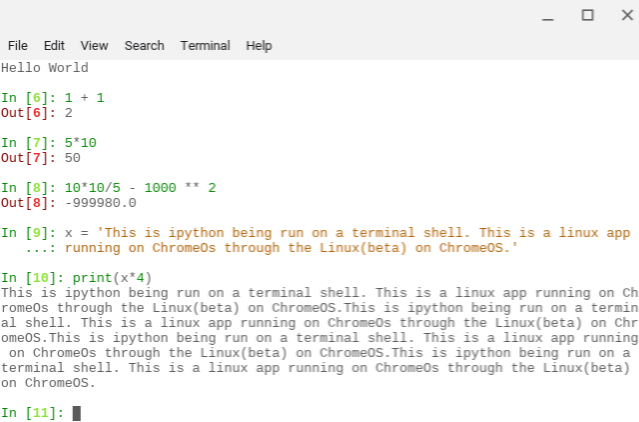
\includegraphics[scale=0.5]{images/chapter-8/ipython_in_shell}
				\caption{Ipython running python operations and printing Hello World and other fun strings.}
				\label{fig:ipython_in_shell}
			\end{figure}
			
			Starting with IPython is relatively simple as the method of installation is easy. However using a console or iPython for learning how to use Python is non-friendly towards beginners as people lacking experience tend to make mistakes with syntax when writing code. This non friendliness is because lines of code are entered one at a time, except for code that is in a nested environment. This is why Integrated Developing Environment (IDE) such as Spyder are recommended as they provide a text editor and console for a quick and simple method of executing the program. Everything shuld be working right out of box after installing Anaconda.
			
			\begin{figure} [!ht]
				\centering
				\def\svgwidth{\columnwidth}
				\Huge
				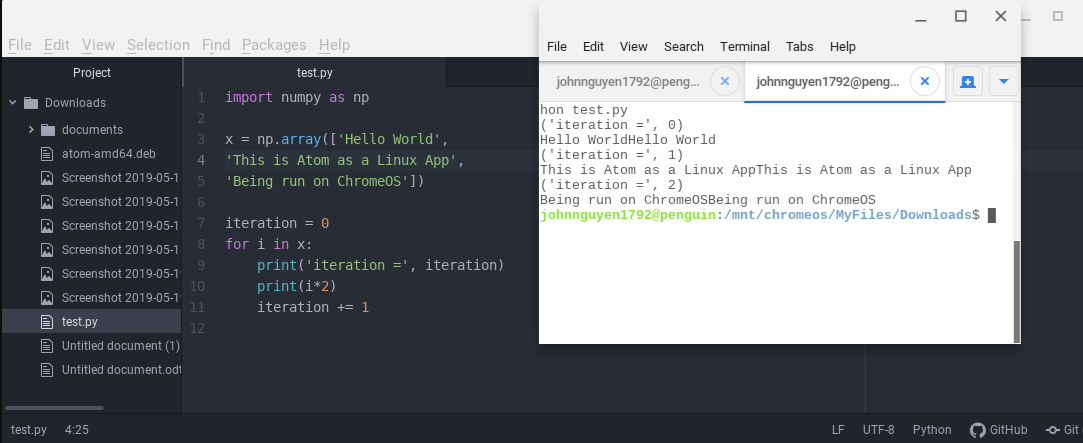
\includegraphics[scale=0.40]{images/chapter-8/atom_IDE_and_ipython}
				\caption{Atom with a Python program open. The program creates a numpy array filled with 3 elements of fun strings. iPython running in a terminal is shown on the left executing the python program with the file name test.py. The output operations prints Hello World and other fun strings in the numpy array as the program iterates through the for loop.}
				\label{fig:atom_IDE_and_ipython}
			\end{figure}	
		
			In this figure, Atom is shown creating a python program which is executed in iPython. The program and its output can be seen in the image. Atom is being used as a text editor to create a Python program. ATOM can be modified to have its own dedicated debugger and console, but this is a more involved process that can result in errors if one lacks computer skills. Alternatively, some terminal can be run by typing "\lstinline|python python_program_name.py|. Using this method requires care with directories. This is because in order to run code from a terminal, you need to understand how to navigate through directories within the terminal in order to run the program. Not so beginner friendly. Again, use Spyder from Anaconda if one is just interested in using Python.
		
		\subsection{Basic Data Types of Python}
			\label{subsec:Basic Data Types of Python}
			Here we introduce the basic data types in Python, numeric, strings, and boolean. The numerical data types are integers, floats and doubles and so forth. In python, knowing the different data types is not that important as Python automatically assigns the variable type based on what is put down in the code. For beginners you can just assume they are numbers types. The next data type is strings which are basically words, letters and statements. We can store sentences in variables with strings. This is done so by enclosing the characters in '' or "".  typically lists. For example, \lstinline{x = 'Hello World'} followed by \lstinline|print(x)| results in Hello World being printed in our console. The most common places to see strings aside from labeling things is storage of data. When files are loaded into Python, data is typically stored in the form of strings, even if the data is numeric. This is because measurements can be separated incorrectly, with spaces, tabs, tags and commas so it is safer to load data into string format since all characters can be represented into a string. With the string loaded, we can parse or analyze the string manually to extract the information into the desired form. An important property strings have in Python is the length and order of the characters in them. Boolean data type is either \lstinline|True| and \lstinline|False|. Boolean are mostly used for logic flow or decision making in general. If we compare two variables for some condition and this condition outputs True, then our code can be designed to go down a particular path, skip a certain path, or end a WHILE loop. Just think of decision trees when considering Booleans.
			
			\begin{lstlisting}[language=Python]
			#numerics
			1, 2.0, 1000000, 25132232.23
			
			#strings
			"a", "bba", "Hello World"
			
			#Booleans
			True, False
			\end{lstlisting}
			
			A more thorough explanation can be found at \url{https://docs.python.org/3/library/datatypes.html}.
		\subsection{Basic Operations of Python}
			\label{subsec: Basic Operations of Python}
			Python is an object oriented language that is indent and line sensitive. These are essentially rules when using Python so that our compiler understand what to do in Python. Object oriented means that taking some variable label such as "a" and you equate it to something such as the number 12, an integer. Indent sensitive means that the indent of the line determines the layer of which the code is executed while line sensitive states that entering a newline means executing a new line of code. These properties become more apparent when we look at C which has different syntax rules for running.  Assignment of the variable to 12 is done by putting in the console or script, a = 12. The variable "a". Now, everytime we pull out the variable a, we get back a 12. With some variables assigned integer objects, we can perform math operations and other tasks. Below is an example of some basic algebraic operations in Python.
			
			\begin{lstlisting}[language=Python, caption=Data types and assignment example]
			a = 5
			b = 10
			c = a + b
			d = a - b
			e = a * b
			f = a ** b
			b / a
			\end{lstlisting}
			
			In the code above, we have performed 5 of many types of operations. Notice how the first line starts with a \#. This is a comment hyphen which tells Python that everything after this is comment meaning it is not to be compiled. Comment are used to describes our program and its contents. It is considered good practice to comment as much as needed. These operations respectively are the addition(+), subtractive(-), multiplication(*), exponential(**), and division(/) operation which are all math operations. The division operation was not assigned a variable and thus running the program above will output value of this operation, 2. Up to the division operation, all the resulting values can be thought of as being assigned to their respective variables on the left. This is assignment operator symbolized by the "=" operator. With the above code excuted, we can pull out the values of operation by inputting the variable into the console. For example, a will result 5, b with 10, c with 15, d with 5, e with 15, f with 9765625 with the last operation having not been assigned to anything. The result of the last operation is  instead outputted when the code is run.
			
			We just discussed math operation so now on to a discussion of boolean operations. Booleans are types of data which embody true and false meaning their properties allow this type of data to check if a value is above some limit, below some limit, or equal to some value. There are more operations but it is not necessary to cover them. Below is a program to illustrate how to use booleans. Like integers, they can also be assigned to variables.
			
			\begin{lstlisting}[language=Python, caption = basic operators of Python] 
			a = 10 > 5
			b = 10 < 5
			var_0 = 5 == 10
			var_ 1 = 5 == 5 
			var_0 != var_1
			\end{lstlisting}
			
			The result operators going from top to down are less than(<), greater than(>), equal(==), and not equal operator (!=). The output of the code is True as the the last operation was not assigned anything so its result is outputted instead. The variables a output True, b with False, \lstinline{var_0} with False, and \lstinline{var_1} with True. A more thorough explanation of operators can be found at \url{https://docs.python.org/3/library/operator.html#module-operator}
			
		\subsection{Basic Data Structures of Python}
			\label{subsec: Basic Data Structures of Python}
			Data structures are objects that contain sets of elements. The most fundamental property of a data structure is their length. The most commonly used lists along with their syntax are \lstinline{lists[]}, \lstinline{tuples()}, and \lstinline|dictionaries{}|. Technically, strings are data structures as well, but Python treats characters and strings the same. For example, the string "Hello World" has a length of 11. 
			
			Discussions will start with lists and tuples first, as they are very similar to each other with only 1 difference and are both simpler than dictionaries. Lists and tuples can be made by simple putting square braces \([]\) and curly braces \{\} around sets of items seperated by commas. The elements do not necessarily need of the same data types. A single list and tuple can contain elements of the numeric types, strings and boolean. The difference between lists and tuples are that lists are mutable and tuples are immutable. In lay man terms, this means that the structure of a tuple cannot be changed when it has been created. However elements within tuples can be modified, removed, elements reordered, etc since they are mutable. Think of mutate and mutations, the ability to change. This mutability of lists make them far more commonly used and by far more useful than tuples.
			
			\begin{lstlisting}[language=Python, caption = Initialization of lists and tuples containing various data types.]
			somelist = [1,2,3,4.0,5,6.0]
			sometuple = ('a','b','c','d')
			a = ['a',2,True]
			b = (100.0, 'b', False)
			c = [True, True, False, False]
			nested_list = [somelist, sometuple, c]
			\end{lstlisting}
			
			The lines of Python above just create lists and tuples of types of the data types. As described in the beginning of the section, data structures have length to them and we will talk more about length when we use the built-in len() function of Python. In order to pull out individual elements of a list or tuple, we attach square brackets at the end of the variable name along with the index number of the element enclosed in the square brackets. For example, in order to obtain the 4th element in somelist, we would call somelist[3] which would give us the number \lstinline|4.0|. In order to obtain a subset of the set of items within the list, we would again attach square brackets at the end input the initial index followed by a colon and the final index. Note that the final index is not shown or included. This is just how Python works. To extract the 2nd and 3rd element in \lstinline|sometuple|, we would call \lstinline|sometuple[1:3]| which would output \lstinline|('b','c')|. Lists and tuples containing other lists and tuples can be created as seen the variable \lstinline|nested_list|. This known as nesting where objects are placed in another object. Nesting can be thought of as putting an object into a container with the biggest container being known as the global. Extracting nested data structure requires the same concepts as extracting individual elements and subset. 
			
			\begin{lstlisting}[language=Python, caption = Printing elements and subsets of already defined lists]
			print(somelist[3])
			print(sometuple[1:3])
			print(nested_list[1][1:])
			\end{lstlisting}
			\noindent Running the above code results in the following outputs
			\begin{lstlisting}[caption = The printed outputs of the elements and subset of somelist and sometupple]
			4.0
			('b','c')
			('b','c','d')
			\end{lstlisting}
			The command \lstinline|nested_list[1]| is the \lstinline|sometuple| nested inside the \lstinline|nested_list|. In short, \lstinline|nested_list[1]| is a list. That is why adding an extra set of square brackets to extract a subset pulls out ('b','c','d').
			
			Python dictionaries are a data structure that has two components for every entry or element, a key and a value. The elements are commonly referred to as a key value pair. The main purpose of a dictionary is to store some value with some associated key which can be pulled out when its uniquely stored key. The order for which the key value pairs are stored in a dictionary is not important and we will see why in a bit. Any immutable object can be a key. Typically strings and numbers are used, but in more complex programs, tuple may also be used. Any data types or data structure, including dictionaries can be stored as a its values while. Enter the dictionary below into the interpreter of choice. 
			
			\begin{lstlisting}[language=Python, caption = Some dictionary that is created]
			value = 100
			some_dict = {
			1:'hello',
			'key':value,
			(1,'key_1'):[1,2,3,4],
			(2):'world'}
			\end{lstlisting}			
			
			When typing in \lstinline|some_dict| into the console, a similar  dictionary f the follow output should be shown, \lstinline|{(1, 'key_1'): [1, 2, 3, 4], 1: 'hello', 2: 'world', 'key': 100}|. Dictionaries, unlike tuples and lists, are unorder data structures. The order the key value pairs of an output dictionary depends on the operating system. 
			
			We have used a key value pairs of numeric an string, string an numeric, tuple an list and tuple an string. Any combination can be used as long as the key is an immutable object. The real use of a dictionary is pulling stored values out of a dictionary with a key. This is done by putting the variable of the dictionary with a single key enclosed in square braces at the end of the variable. For example, \lstinline|some_dict[1]|results in the string \lstinline|'Hello'|. The value of the key can be modified anytime, but the key will always be the same. Modification of the key is the same as pulling out its value via its key but with the addition of using the assignment operator \lstinline|=| followed by a value. This is why value of a dictionary can be any object while keys can only be immutable property, strings and numerics. Also since we just pull out a value or assign a new value using its associated key, the order of the key value pairs are not necessary. Altogether, the properties make dictionaries extremely fast and light weight on memory. Here is the dictionary being worked with in an iPython console in a terminal. 		For better details of data strucuture, visit \url{https://docs.python.org/3/tutorial/datastructures.html}.
			
			\begin{figure} [!ht]
				\centering
				\def\svgwidth{\columnwidth}
				\Huge
				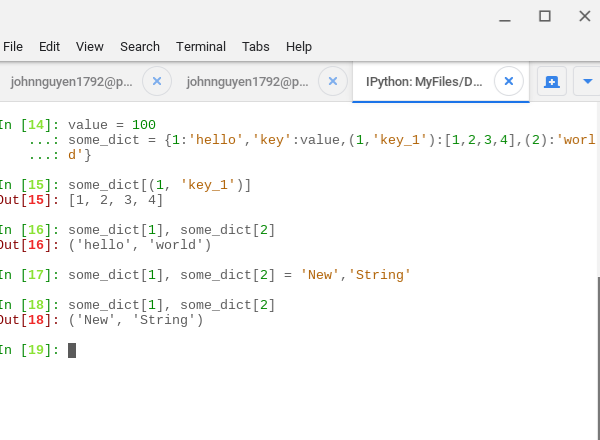
\includegraphics[scale=0.5]{images/chapter-8/dictionary_python_example}
				\caption{Ipython running python operations and printing Hello World and other fun strings.}
				\label{fig:dictionary_python_example}
			\end{figure}
		
		\subsection{Functions, Methods and Arguements in Python}
			\label{subsec:Functions and Arguements in Python}
			In programming, functions are tools that execute some computation or code when called up. Functions are some keywords in the namespace that followed by parentheses\lstinline|()|. Arguments are the inputs of the function that go inside the parentheses. 
			
			\begin{lstlisting}[caption = Function structure]
			function_name(argument_0, argument_1, argument_2)
			\end{lstlisting}
			
			Functions have a wide array of uses in Python such as declaring a variable data type, changing a data types, performing mathematical computations, describing the length of a string etc etc.  The following example of a Python function that is covered has an output to initially demonstrate the similarity between a mathematical function and a Python's version of function as an analogy to mathematical functions. A warning, Python functions are not required to have an output. The mathematical function f of x and y, $f(x,y)=xy+2y+5x$, in terms of a Python function would be defined as the function f() that accepts two arguments to return the output equal to \lstinline{x*y+2*y+5*x}.
			
			\begin{lstlisting}[language=Python, caption = Defining a function in Python that performs arithmetic.]
			def f(x,y):
				output = x*y + 2*y + 5*x
				return output
			\end{lstlisting}
			
			In Python, functions are always defined by the keyword \lstinline|def| followed by the name of the function and parentheses enclosing its parameters and ending with a colon. The following code that is declared to be nested or belonging to the function f(x,y) done by a single tab. The code that is nested into the function is known as the function's local scope. In the example, the function f is part of the global scope, the highest and most fundamental level of scope. All local scopes must even connect to the global scope. The output of the function is returned by the keyword \lstinline|return|. For functions with a returned output, we can assign the returned output to a variable by using the assignment operator, like so \lstinline|z = f(2,3)|.
			
			It is also possible to create a functions that do not return anything, such as printing some output or transforms a variable.
			
			\begin{lstlisting}[language=Python, caption = Other types of functions in Python that do not return some output or variable.]
			def p(x,y):
				output = x*y + 2*y + 5*x
				print('The output of f(x,y) is', output)
			
			def g(x,y):
				output = f(x,y) * 10
				return output
				
			def t(some_data_structure):
				del some_data_structure[-1]
			\end{lstlisting}
			
			The function p(x,y) just prints the same arithmetic done in function \lstinline|f| but instead print the value out as a string. If we tried assigning some variable to the function p(x,y), we would get an error since the function does not return anything because of the lack of the \lstinline|return| keyword. In short, there is nothing to assign to the variable. The function g(x,y), calls the function f(x,y) and takes it's parameters and input them into f(x,y) and into and puts them into f(x,y) for f(x,y) to use. This would be mathematically equivalent as stating $g(x,y)=10 \times f(x,y) = 10(x*y + 2*y + 5*x)$. The final function is unnecessary, but the keyword del, which is used to delete objects, is placed into the function \lstinline|t(some_data_structure)| so that it deletes the final element in that data structure. We know the code within a function ends when the next non empty line is tabbed into the same level as the defined function. 
			
			The examples of functions we covered are user defined function, hence where the \lstinline|def| comes from. Python also has built in functions which can be found at \url{https://docs.python.org/3/library/functions.html}. Some commonly 
			
			\begin{lstlisting}[language=Python, caption = Python's builtin function. We can also call builtin functions from within builtin functions as demonstrated]
			x = [1,2,3,4,5,6]
			print(x)                  # Prints the arguement in string form
			print('length =', len(x)) # Returns the number of element in the data structure
			print('min(x)=', min(x))  # Returns the minimum value of the data structure
			print('max(x)=', max(x))  # Returns the maximum value of the data structure
			\end{lstlisting}
			
			Methods are built in functions of data types, functions and classes, or more generally objects. This means that stored contents within a variable or object can access the methods available to the class of objects. The more commonly used methods are the \lstinline{append()} method of lists and the \lstinline{split()} of strings. The append method attaches the object in its argument to the end of the list while the split method splits a string into a list where the argument is the break point character. To use an objects method, we attach \lstinline|.methodname()| to the end of the object. 
			
			\begin{lstlisting}[language = Python, caption = Examples of append and split methods of lists and strings]
			somelist=[[1,2,3,4]]
			somestring="Hello+world+Nice+to+meet+you]
			listofbooleans = [True, False, True, True]
			somelist = somelist.append(listofbooleans)
			splittedstring = somestring.split('+')
			\end{lstlisting}
			\noindent The following program shows simple execution of the methods. Keep in mind that that variables were used as argument, but we could have directly input the data objects like so, \lstinline|somelist = somelist.append([True, False, True, True])|, to achieve the exact same result. Methods can also be applied at the end of the object as opposed to the variable, to achieve the same result. \lstinline|somelist = [[1,2,3,4]].append([True, False, True, True])|. When working with Python, what matters is the data type of the object. For most of this book, we treat variables as containing objects, but in reality variables point towards objects. Which means when a variable is used as an argument, the object is actually being used as the argument as the variable just points to the object. That is why all of these input result in the same outputs because the are all identical minus the pointing effect of variables. This makes working with Python easy, but there are some side bad effects of designing Python this way. The simplest way to think is to just assume the variables contain as opposed to point, whichthis book will assume. 
			
			\begin{lstlisting}[caption = Transformation of the new lists]
			somestring now has 
			[[1,2,3,4], [True, False, True, True]] as opposed to 
			[[1,2,3,4]].
			
			splittedstring now contains the  
			["Hello","world","Nice","to","meet", "you"]
			\end{lstlisting}
			
			Also notice how we used the assignment operator to assign the list variable and a new variable to the methods. This is because, Python methods behave just like Python functions meaning that they only return new object. If we want to keep this newly returned object, we have to assign it by replacing the old object with the new object or assigning the returned object to a new variable. 
		\subsection{Loops and If Statements in Python}
			\label{subsec:Loops and If Statements in Python}
			Now jumping into the real meat of programing, loops and lists. Computers and programs were created to perform redundant tasks faster and more reliably than a human ever could. In computer language, this can done by going through some collection of items and repeating some task until we are out of elements and/or until some condition is met. In programming languages, these repeated tasks are called loops and a collection of objects are known as lists objects.
			
			Loops can be thought of as types of container that will execute the same code in their respective containers over and over until some condition is met. The number of times the code repeats itself is known as numbers of iteration where the ith iteration is the ith time the code runs. The types of conditions for termination of the loop depends on the types of loop, FOR or WHILE loops. While one may technically just stick to one type of loop, different situations may intuitively favor one of the loops. The best way to explain loops and list objects for  beginners is by example. 
			
			We start off with a FOR loop which requires a list object. The example below begins iterating through a range(interger) list object until it goes through the entire list.
			
			\begin{lstlisting}[language=Python, caption=For loop example]
			j = 0
			k = 0
			for i in range(5):
			  print('iteration =', i)
			  j = j + 1
			  k = k + i
			  print('j =', j)
			  print('k =', k)
			\end{lstlisting}
			
			The line "for i in range(5)" states that the FOR loop will iterate through the range(5) object until the last element. The code being executed within this FOR loop must be nested into the loop. As mentioned earlier, this is done by indents. As stated earlier, loops can be thought of as containers an the nested code is inside the inside the container. When it reaches a line of code that is no longer indented or nested into the loop, begins the next iteration with the first nested line being executed again and terminates if there are no more elements left in the list object. The number of times the code nested into the loop is 5 iterations for the objects 0,1,2,3,4 inside the range(5). With each iteration setting the variable "i" to be the current element in the list object. 
			
			Now onto what the code is doing. We first take two variable j and k and assigned them both 0. This is known as initialization. Variables must be initialized before we can perform operations on themselves. The FOR loop then adds 1 to j and i to k with each iteration. Notice how 0 is the first index and not 1. This is because Python starts at 0 when indexing. Some languages use 1 while others use 0 like Python. Meaning the first iteration i is 0 while last iteration is 4, not 5. The last interation is 4 because of the fact that Python starts index at 0. I am repeating this because it can be confusing for beginners. 
			Remember that for each iteration, the code starts back at the first line in its nested block of code. The resulting output of the loop is
			\begin{lstlisting}[caption=For loop output]
			iteration = 0
			j = 1
			k = 0
			iteration = 1
			j = 2
			k = 1
			iteration = 2
			j = 3
			k = 3
			iteration = 3
			j = 4
			k = 6
			iteration = 4
			j = 5
			k = 10
			\end{lstlisting}
			
			Starting the WHILE loop example, WHILE loops check for the boolean status for True or False to signal termination of the loop. FOR loops have a finite number of iterations, ie they have an upper limit on the number of times they will repeat a block of code based on the length of the input data structure. WHILE loops can be run indefinitely, or forever, until a condition is met. In some cases, the code is meant to be run for ever and there are no conditions for termination as a result.
			
			\begin{lstlisting}[language=Python, caption = While loop example]
			i, j, k = 0, 0, 0
			while i < 5:
			  print('iteration =',i)
		      j += 1
			  k += i
			  print('j =',j)
			  print('k =',k)
			  i += 1
			\end{lstlisting}
			
			The output of this code is exactly the same as the FOR loop example, the only difference is the way we structured the code which arise because of the differences in the nature of the code. One key difference between the FOR and WHILE loop is the last line of code in the while loop. The variable i is increased by 1 every iteration whereas in the FOR loop it was assigned the value of the elements in the range(5). With every iteration of the WHILE loop, the value of i is checked to see if it is less than 5. If it less than 5, then we continue to the next iteration. This continues till i is not less than 5, which then results in termination. The rests of the difference are just different syntaxes for executing the same things.
			
			Finally to talk about if statements. Like WHILE loops, conditions are checked to see if they are True or False to decide which blocks of code to execute or to not execute any code at all. You can think of this as a flow chart. If so and so is True then do do this, if False then proceed down this path. Many if statements can be nested within in each other to produce complex "decision making trees".
			
			\begin{lstlisting}[language=Python, caption = Conditionals]
			a = 10
			b = []
			if a < 5:
			  print('a is less than 5')
			elif a = 5:
			  print('a is equal to 5)
			  b.append(a)
			  if a in b:
			    print('a is in the list b')
				else:
				  print('a is not in list b')
			else:
				print('a is more than 5') 
			\end{lstlisting}
			
			The above tree is not complex, but it contains an example of a nested loop with some new operations. This if statement just checks the value of a and prints out its relative relation to the number 5. If interests in what is and what b.append() does, then look up lists and methods in Pythons. The line \lstinline|if a in b| checks to see if the object \lstinline|a| exists in list b. When we initialized \lstinline|b|, we initialized it as an empty list.
			\subsection{Global and Local Scope}
				\label{subsec:Global and Local Scope}
				As mentioned in the Python introductory section \autoref{sec:Python} and in the previous section on functions, \autoref{subsec:Functions and Arguements in Python}, scope is the hierarchy of the code. When a line of code is said to be nested into something, it is defined to be the in the local scope of that said something. For example, the global scope is the first and foremost level when creating a new program. We can define as many functions, loop or classes, as need be in the code and each function, class or loop would have their own local scope. Each local scope can in turn have their own scope as seen in the function g(x,y). Within the global scope, we defined the function \lstinline|g| and within g(x,y)'s scope is the function f(x,y) which in turn has its own local scope. In programming, this kind of hierarchal leveling is known as nesting where we have local scopes within local scopes within locals until we reach the fundamental global scope, which all scopes are connected to. %make image of tree
				
				\begin{figure} [!ht]
					\centering
					\def\svgwidth{\columnwidth}
					\includegraphics[scale=0.70]{images/chapter-8/scope_diagram}
					\caption{The global scope sits at the top of the tree and is given the level 0. Any variables or keywords defined in the global scope is available to all scopes below it. The functions and loop defined in the global scope have their own scopes which are defined to be in level 1. In level 1, only local 2 does not have any scopes below it. Likewise, the functions, loops and conditionals in local 1 and 3 have their own local scopes, numbered 4, 5 and 6. Any variable or keywords defined in local 1 are available only to local 4, but the reverse is not true meaning any variables defined in local 4 are not available to local 1. }
					\label{fig:scope_diagram}
				\end{figure}
				
				What are inherent properties because of scope level? Any variable, function or packages declared or defined within a given scope is available in that and scopes lower than it. The inheritance of variables and structures is a one way direction. Scopes higher than its children scope do not inherit the defined variable or structure. This means that any variable called within the global scope is available to all scopes since every scope must be below the global scope. However, the global scopes inherits no variables defined in any of the scopes below it. So if we tried to call a function defined in local 1 while we are in the global scope, we would get an error since the global scope does not inherit any variables or structures from anything below it. Local 1, Local 2 and Local 3 all belong to level 1 but they are each their own separate scopes and since none of them are connected to each other, variables defined within one the scopes is not available to the other scopes despite being in the same level. For example, the function that is defined in Local 3 is only available to be called in Local 1, it is not available to be called in the local 1 or local 2 scope. 
				
				Levels are represented in our Python program by the number of tabs or indents in a given line. The level n requires our line of code to have n tabs so therefore all level 1 scopes require 1 indent. Below is a "cartoon" Python program that describes and "illustrate" the hierarchy of Python. It is a "cartoon" program because you should not try to run it. 
				\begin{lstlisting}[language=Python]
				global scope with level 0
				a = 1
				def function_name_0:
					b = "string"
					local scope 1 withing level 1 inheriting the variable "a" from the 
					global
						def nested_function_name_1:
							somelist = [True, False]
							Local scope 4 with level 2 inherenting variables "a" and "b" 
							from scope 1
							
							Local scope 4 inherits the variable "a" since local scope 1 
							inherited it from global
							
							The variable some_list is not available to any other scope, 
							however the variables a and b are callable within scope 4 
				
				def function_name_1:
					local scope 2 within level 1
					c = ["Hello", "World"]
					Local scope 2 inherits variable "a" from the global scope
					Because local scope 2 is isolated from all other scopes, nothing 
					inherits
					the list "c"
					
				for element in [1,2,3,4,5,]: 
					local scope 3 within level 1
					d = True
					some_tuple = ['a','b','c','hello']
					while True:
						Local scope 5 within level 2 inheriting variables "a" and "d"
						Does not inherit variable "e" and "more_lists" from scope 7
						some_dict = {'key', 'value'}
					for j in some_tuple:
						local scope 6 within level 2 inheriting variables "a" and "d"
						Does not inherit variable "e" from scope 7
						more_lists = [1,2,3,4]
						
					if d == True:
						Local scope 7 within level 2 inheriting variables "a" and "d"
						Does not inherit the list "more_lists" 
						e = "Hello World"
						print(some_tuple)
						
				\end{lstlisting}
				
			\subsection{Folder and File in Python}
				\label{sub:Folder and File in Python}
				This section is dedicated to using explaining how to implement an use a basic directory system, basic navigation through folders, and opening files in Python. It is not necessary to learn the intricacies of folder navigations or all the commands for doing so. In fact, different operating systems have different commands for moving through folders. In Python, we open a file with the function \lstinline|open()| where the required argument is a string of the location of the file relative to the folder the main program is in. The argument of the function depends on the operating system that is being used. Therefore, the syntax of the argument used to open the file would be different for different operating systems despite using the same folder structure. 
				
				To begin opening a file, you must know where it is located within the computer. When we look for a file, we open folders and folders within some explorer until we reach the desired files. The difference now, is we must open navigate through folders with a terminal or typing in commands. To simplify this part, we will use "good" folder structure. We will define the folder that the program is located in to be the global folder. Any folders within this global folder will be its local folder. Does this sound familiar? Refer to \autoref{subsec:Global and Local Scope} to understand level and scopes. The local folders should have names such as "images" for the image files, "data" for the data files and "documents" for the document files. Do not put everything into the global folder, it will be incredibly messy to work with. By working in the global folder, a file within one of the local folders can opened in the program by calling the function \lstinline|open("/images/image_file.png)| or \lstinline|open("/data/data_file.text)|. As long as you work within the global folder, it will be easy to open any file in any of the local folders. Since simple folder names and "good" folder structure, it is not necessary to move between the folders as one can easily remember the folder a file is in.
				
				\begin{lstlisting}[caption= Cartoon of the directory structure]
				global folder with the main program file
					images folder
						image0.png, image1.svg, image.jpeg
					data folder
						data_0.text, data_1.csv, data_2.tsv
					articles
						article_0.pdf, article_1.doc
				\end{lstlisting}
				
				If we were to open or load image0 in the images folder while we are in the global folder, we would call the open function with arguments detailing the location of the file relative to the global folder. This is done by calling the code \lstinline|open("images/image0.png")|. If we were to open the \lstinline|image0.png| while within the data folder, than things become a bit more complicated as we would have to move back to the global folder from the current local folder and then into the image folder. This would be done so by  \lstinline|open("../images/images0.png)|. The addition of ".." at the start of the argument indicates that we are moving back up one directory, which would be the global folder. As long as you stick to a simple folder system and stay within the global folder, it is only necessary to remember how to open a file relative to the global space. This greatly reduces the amount of knowledge and commands required to load and open a file within the Python program. 
				
			\subsection{Parsing Files in Python}
				\label{sub:Parsing Files in Python}
				With the knowledge to open a file using Python, we can begin parsing our file. Parsing just means to analyze a strings. The simplest method of parsing a file would be assign our opened file to a variable. Because we are working from the global directory, we know that data file must be in the \lstinline|"data"| folder. The name of the file is \lstinline|"data0.txt"|. We will create variables with these labels to store the path of the file to demonstrate the general basics to opening a file. The data in our data file of contains the following contents when opened in some text editor. 
				
				\begin{lstlisting}[caption=The contents of the raw data file.]
				Hello World.This is a data file
				Here is some simple data
				1 2 3 4 5 6 7 8 9 0
				11 12 13 14 15 16 17 18 19 20
				91 92 93 94 95 96 97 98 99 100
				90 89 88 87 86 85 84 83 82 81
				\end{lstlisting}
				
				The data file has 5 lines of text. The first two lines could be interpreted as header data of the data file that is typically produced by instrumentation. Only the numeric numbers are of interested, so parsing of the data file is required extract what is desired. Using the \lstinline|open()|, we load all the contents into the the variable \lstinline|filecontents|.
				
				\begin{lstlisting}[language=Python, caption = The data file being opened in python and passed on to]
				directory = "data/"
				filename = "data0.text"
				filecontents = open(directory+filename)
				\end{lstlisting}
				
				By assigning the directory and name of the file into the variables \lstinline|directory| and \lstinline|filename|, we can easily replace the variables with new file names and directory to easil reuse the code for another file. In the arguement of the \lstinline|open()| function, we concatenated the \lstinline|directory| and \lstinline|filename| variables to effectively create the pathway to file relative to the global directory.
				The following contents of \lstinline|filecontents| will contain 5 strings inside a list, one for each line within the text file.
				
				\begin{lstlisting}[caption = {contents of filescontents variable}]
				["Hello World.This is a data file",
				 "Here is some simple data",
				 "1 2 3 4 5 6 7 8 9 0",
				 "11 12 13 14 15 16 17 18 19 20",
				 "91 92 93 94 95 96 97 98 99 100",
				 "90 89 88 87 86 85 84 83 82 81"]
				\end{lstlisting}
				
				Data typically contains header information, such as date, time or sentences, that makes parsing it with the built in functions specifically designed to open csv, tsv or tags separated data files difficult. Let say the first 2 strings are header data and the line containing our data is the third line to the final line. A variable called \lstinline|rawdata| is assigned the last 3 elements of our data, ignoring the header lines. With a for loop, we can separate each number within a single string into a list of elements where the spaces that separate the elements are the breaks. We also have to convert the str elements of numbers get converted into numbers. Since we are dealing with integers, we choose the int data type. If any of the elements have decimals, then we would use float data type. Also in other data files, the breaks between the data could be a comma or a tab hence the file types comma separated values (csv) and tab separated values (tsv). The following code will show the finishing touches of parsing the simple data file.
				
				\begin{lstlisting}[language=Python, caption = Iterating through the raw data to create the final data]
				rawdata = filecontents[2:]
				data = list()
				for line in rawdata:
					line = line.split(' ')
					line = list(map(int, line))
					data.append(line)
				\end{lstlisting}
				
				This part of the program takes the last 3 lines containing our data and stores them in a new variable called \lstinline|rawdata| and we initialized a new variable, \lstinline|data| with the \lstinline|list()| function. We then use a for loop to iterate through the \lstinline|rawdata| and transforming the line variable from a string, to a list of numerical strings, and to a list of integers. With the list of integer, we append it to list variable, \lstinline|data|. And there we have it, our \lstinline|data| list variable now contains our data in the form that we want.
				
				\begin{lstlisting}[language=Python, caption = Contents of the data variable]
				[[1, 2, 3, 4, 5, 6, 7, 8, 9, 0],
				[11, 12, 13, 14, 15, 16, 17, 18, 19, 20],
				[91, 92, 93, 94, 95, 96, 97, 98, 99, 100],
				[90, 89, 88, 87, 86, 85, 84, 83, 82, 81]]
				\end{lstlisting}
	\section{Getting Started with Markdown}
		All one needs to understand about Markdown to be able to understand its syntax in plain text and whether a program or platform supports it. Markdown is a type of typesetting language that was created for the web, but has been adapted for creating semi elegant documents. Simply put, Markdown uses plain text to create richer documents. This is done by following the syntax of Markdown. Not all the syntax is simple, but it is not necessary to memorize the more complicated syntaxes such as embedding videos. Jupyter project supports Markdown as well as Python making it possible to create notes and code together in a single file. In fact, Jupyter supporting markdown is the only reason a section on Markdown is included in this book. There are other source of MarkDown editors, but this book just discusses Jupyter. 
		
		The history and where the syntax comes is not that important as not everyone is in web development. If Markdown does not seem worth the effort to pick up, then it is best to stick with other note taking platforms such as Onenote, Google Keep, Evernote etc. However by learning MarkDown, one will be able to make beautifully laid out Jupyter notebooks for their project.
		
		To start off learning Markdown, there is no place to start off. There really is no right way or fundamentals to follow when use Markdown. Everyone has created a document before, but now you have to do so with Markdown using plain text. In Markdown, you can create headers, tables, input images, links, videos, bullets for lists all in plain text. Markdown is not as creative and powerful as other document editors, but it is light weight, simple and low on resources, making it accessible to everyone on any platform. Once the document is ready, you begin compiling and the richer documents should be ready. Some of the syntax can get complicated, but luckily it is not required to memorize all of them as one can quickly reference this sheet at \url{https://github.com/adam-p/markdown-here/wiki/Markdown-Cheatsheet}. Feel free to just copy the template and replace the parameters with the desired texts. Here are some plain text being converted into a MarkDown document.
	
		\begin{figure} [!ht]
			\centering
			\def\svgwidth{\columnwidth}
			\Huge
			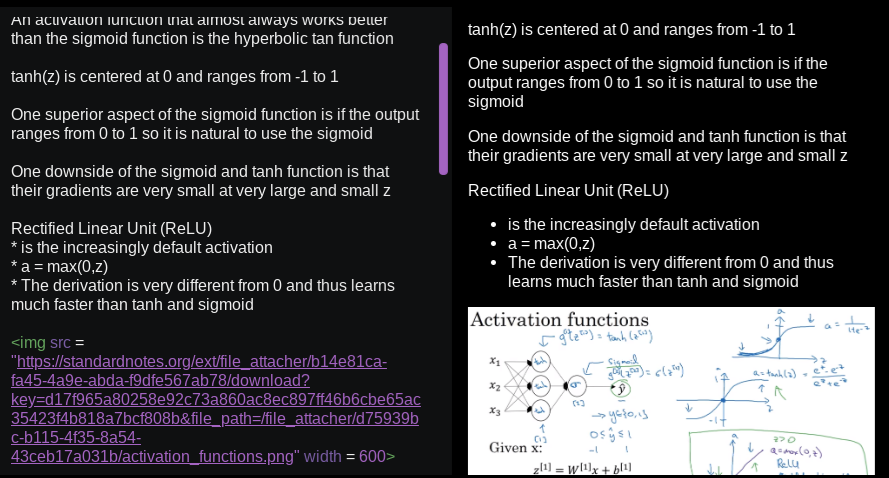
\includegraphics[scale=0.5]{images/chapter-8/markdown_1}
			\caption{This is done in some editor that converts plain text into MarkDown. The name of the editor will not be mentioned.}
			\label{fig:markdown_1}
		\end{figure}
	
		You just start working on a document until it is to standards. We only included images of a plain text file being converted into a Markdown document file. Examples of Markdown will be shown again in the Jupyter section. There will be explanations of how to build beautifully and elegantly laid out Jupyter notebooks. This is important as flow of information is incredibly important when designing a book or document such as this.
		
	\section{Basics of C for Arduino}
	\section{Databases and SQLite3}
\chapter{Essential Programming Packages}
	\label{chp:Essential Programming Packages}
	This chapter is about the essential packages used in creating a project and performing research. It is highly recommended to understand the contents of the previous Chapter\ref{chp:Fundamentals of Recommended Programming Languages}. The first section will discuss the SciPy stack, the scientific Python computing ecosystem, and only delve into its cores packages. These packages are Numpy, Scipy. Matplotlib, iPython, Jupyter, and Pandas. There are other packages, but they should only be learnt if one needs them. 
	The most common trends for using these packages is because their operations are done in a more efficient language or program. For example, matplotlib is matlab that has been packaged so that Python can utilize it's plotting capabilities. Other packages include iPython and Jupyter which provide us with a workspace to write and test out our code. The most important is Jupyter, which is an extended version of iPython. The star of the next chapter is Jupyter.
	\section{Python Standard Library Packages}
		\label{sec:Python Standard Library Packages}
		These packages come built into Python so it is not necessary to import or install any additional packages if base Python is installed. The packages in the standard library are much more involved than the community packages, however we cover a few of these packages as they help us in our data gathering. The standard libraries packages also tend to be slower and thus are avoided when better support community packages are available. The next section, \ref{sec:Scientific Python Stack}, why we avoid the standard library when possible.
		\subsection{datetime}
			\label{subsec:datetime}
		\subsection{sqlite3}
			\label{subsec:sqlite3}
		\subsection{copy}
			\label{subsec:copy}
		\subsection{os.path}
			\label{subsec:os.path}
		\subsection{urllib}
			\label{subsec:urllib}
		
			
	\section{Scientific Python Stack}
		\label{sec:Scientific Python Stack}
		\subsection{Numpy}
			\label{subsec:Numpy}
			Long story short, iterating large lists with loops in Python is slow, therefore we use perform array calculation in Numpy using structures known as numpy arrays. Calculations with numpy arrays with the Numpy packages are faster because calculations in Numpy are done in C. This is known as wrapping where we use one programming language to interact with another programming language. This Python wrapper allows our Python code to interact with the results done in C. This gives us the speed and power of C with the convenience and simplicity of Python. As stated in the previous chapter, C is a compiled language and therefore more fundamental then Python making it faster and more efficient than Python. Using a wrappers allows us to take advantage the superior performance in C, while allowing us to write our code in our desired language. This is a common trend in most packages of Python. Python itself is a slow language, but its universalness allows it to utilize programs and libraries of other languages and programs, in particular C. This compatibility and wrapping is done by 
			
			In order to to utilize the numpy package, we must import it into our environment. This means loading all of the numpy operations, methods, functions and data structures code so that we can use.
		

\chapter{Experimental Techniques}
	\label{chp: Experimental Techniques}
	\section{Modulation and Heterodyne Principle}
		\label{sec:Modulation and Heterodyne Principle}
		Modulation and heterodyning are techniques typically used in series to modify or transform a signal of some sort into another form that is more readily detectable and useful. For example, in the PDH locking technique, the carrier beam is modulated to generate sides bands which create a signal in the back reflection. The detector signal from the back reflection is then heterodyne with a local oscillator to produce the PDH error signal for locking.

		\subsection{Modulation}
			\label{subsec:Modulation}
			This section is to provide basic knowledge of modulation of a carrier waves and the heterodyne principle to aid in understanding of the complicated techniques used in this experiment, particular (so far) for Pound-Drever- Hall locking technique. Modulation and demodulation is a technique that is widely used in telecommunications, such as in cellphones and radio transmissions, to efficiently extract small of information stored in the modulation. Experimentally, this modulation data is stored in the spectral transition data for frequency modulation spectroscopy and NICE-OHM spectroscopy, the error signal of Pound-Drever-Hall locking technique and the more basic lock in amplification.
			
			The essential idea is to encode information in electric field of electromagnetic radiation either in the amplitude, frequency, or phase. This can be done by varying the power of the laser or by the use of nonlinear crystals. Here a simple plane wave traveling in some arbitrary direction. The magnitude of the modulation is define as the modulation depth/index which is denoted by $\beta$.
			
			\begin{equation}
				\tilde{E}(t)=\left(A_o\right)e^{i(\left[\omega_c\right] t + \left(\phi)\right)}
			\end{equation}
			
			Amplitude modulation involves varying the amplitude of wave with time such as with a sine function, $A(t)=\beta \sin{\Omega_m t}$ which will result in
			
			\begin{equation}
				\tilde{E}_{Amplitude}(t)=A_o\left(1+\beta \sin{\Omega_m t}\right) e^{i(\left[\omega_c\right] t + \left(\phi)\right)}
			\end{equation}
			
			Time varying the frequency/wavelength with a sine function will result frequency modulation
			
			\begin{equation}
				\tilde{E}_{frequency}(t)=\left(A\right) e^{i(\left[\omega_c (1+\beta \sin{\Omega_m t}\right)] t + \left(\phi)\right)}
			\end{equation}
			
			And finally phase modulation, the modulation technique of most interest in this thesis
			
			\begin{equation}
				\tilde{E}_{phase}(t)=\left(A\right)e^{i(\left[\omega_c \right] t + \left(\beta \sin{\Omega_m t})\right)}
			\end{equation}	
				
			The given equations are the time domain signals but the action of the modulation can be better described in their frequency domain. With the case for phase modulation, as long as the modulation index,$\beta$, is small, first order sidebands with $\omega \pm \Omega $ will be generated. Higher order sidebands containing interger multiples of $\pm \Omega$ are also present but are ignored as they contain higher orders of the modulation index which is assumed to be very small. More rigorous proofs can be seen in FM spectroscopy paper \cite{FMspec} and PDH locking technique paper \cite{PDH Intro}. In short, there are only 3 important frequencies after phase modulation to most techniques using phase modulation: the carrier frequency $\omega_c$ and two side bands $\omega_c$ 
			
			\begin{equation}
				\tilde{E}_{phase}(t)\approx E_o [e^{i\omega_c t}   +   \dfrac{\beta}{2} e^{i(\omega_c +\Omega_m)t}  -  \dfrac{\beta}{2} e^{i(\omega_c -\Omega_m)t}]
			\end{equation}
			
			Include picture with carrier frequency and side bands with frequency noted here
			This transformation from the time domain phase modulated to side can be described via a taylor expansion about the carrier frequency with modulation depth, $\beta$, assumed to very small. Alternatively, a more complicated calculation with a fourier transform can be done. I have yet to try the fourier transform.

		\subsection{Demodulation by Heterodyne Principle}
			\label{subsec:Demodulation by Heterodyne Principle}
			The Heterodyne principle is action of multiplying or mixing two sinusoidal waveforms which can be also be expressed as a sum of two sinusoidal waveforms whose frequencies are given by the sum and difference of the two mixed waveforms.\cite{MITModulation}. For example, if a photo-current from a photo-detector contains some sinusoidal components with a defined modulation frequnecy, then it can be extracted via the use of the Heterodyne principle. This is known as demoulation where we extract the information stored from the modulation. With some current signal containing two sinusoidal components of the same frequency, $\Omega_m$.
						
			\begin{equation}
				I_a(t)=I_1 (t) +I_2 (t) I_{noise}(t)= A_1 \cos{\Omega_m t} + A_2 \sin{\Omega_m t} +\sum_{\omega_i}^{} a_i \cos{(\omega_i t + \phi_i)}
			\end{equation}
			
			The \text{$I_1(t)=A_1 \cos{\Omega t}$} or \text{$I_2(t)=A_2 \sin{\Omega t}$} term can be extracted by demodulation via the use of the Heterodyne principal by mixing the photo-current signal with a sinusoidal current from a local oscillator of frequency $\Omega_{lo}$ with some phase $\phi_{lo}$. The noise terms will result in 0 signal after heterodyning so they will be ignored here on out.
		
			\begin{equation}
				\begin{split}
				I_b(t) &=I_a(t) \times B\cos(\Omega_{lo}t +\phi_{lo}) =(I_1 (t) +I_2 (t))*B\cos(\Omega_{lo}t +\phi_{lo}) \\
				& = A_1 B \cos{(\Omega_m t)}\cos(\Omega_{lo}t +\phi_{lo}) + A_2B \sin{(\Omega_m t)}\cos(\Omega_{lo}t +\phi_{lo}) \\
				& = \dfrac{A_1 B}{2} \left[ \cos{\left(\left(\Omega_m+\Omega_{lo}\right)t+\phi_{lo}\right)}  + \cos{\left( \left( \Omega_m - \Omega_{lo} \right)t +\phi_{lo}        \right)}                                    \right]\\
				& + \dfrac{A_2 B}{2} \left[ \sin{\left(\left(\Omega_m+\Omega_{lo}\right)t+\phi_{lo}\right)}  + \sin{\left( \left( \Omega_m - \Omega_{lo} \right)t -\phi_{lo}        \right)}                                    \right]\\
				\end{split}
			\end{equation}			 
		
			The goal now after mixing with the local oscillator is to rid of the plus combination of the two waveforms. With current in this form, this can be done with a low pass filter which will filter out high frequency components, ie the plus combination of the two sinusoidal waveforms.
		
			\begin{equation}
				I_c(t) = \dfrac{A_1 B}{2} \left[\cos{\left(\left(\Omega_m-\Omega_{lo} \right)t +\phi_{lo}\right)}\right]
				+\dfrac{A_2 B}{2}\left[\sin{\left(\left(\Omega_m-\Omega_{lo}\right)t-\phi_{lo}\right)}\right]
			\end{equation}					
			
			If we tune the local oscillator frequency so that frequency is equal to the modulation frequency and set the phase to be 0, ie $\Omega_{lo}=\Omega_m$ and $\phi_{lo}=0$, then we have obtained a dc component representation of the cosine term. This dc component can also be amplified for easier detection.
		
			\begin{equation}
				I_d(t) = \dfrac{A_1 B}{2}
			\end{equation}	
		
			If say, we instead set the phase of the local oscillator to be 90 degrees out of phase, ie $\cos(\Omega t + 90^o)=\sin(\Omega t)$, then we can extract the sine component of $I_a(t)$.
			
			In summary, by mixing a signal containing various waveforms of various frequency with a reference waveform of variable frequency and phase, the individual waveforms components can be experimentally extracted. To chemist who like with quantum mechanics, this is analagous to operating a general wave function with a state projection operator to obtain the component weight of the state.

	\section{Feed Back Control Theory}
		\label{sec:Feed Back Control Theory}
		asadfasdf talk a bit about feedback loops, include the book used for feedback control theory

	\section{Pound Drever Hall Locking Technique}
		\label{sec:Pound Drever Hall Locking Technique}
		
		\begin{figure} [!ht]
			\centering
			\def\svgwidth{\columnwidth}
			\resizebox{160mm}{!}{\imginput{images/PDH-setup.pdf_tex}}
			\label{fig:PDHSetup}
			\caption{a) is a cartoon showing a ray of light bouncing back and forth in a Fabry-Perot cavity while interacting with a sample. b) Illustrates a realistic interaction a resonating beam with a sample }
		\end{figure}
		
		The locking of a cavity refers to locking one of the cavity modes to the frequency of the laser beam so that optical power build may resonate and build up in optical power.
		The locking technique utilized is Pound Drever Hall (PDH) technique with high frequency modulation. This method of locking the lasing system was chosen due to its high sensitivity about the cavity resonance, fast response to frequency fluctuation and its ability to distinguish which side of the cavity resonance the laser frequency is relative to resonance \cite{PDH Intro}. The cost of utilizing this technique is the accompanied difficulty and complexity of this technique but a tight lock is required to minimize locking noise due to frequency modulation to amplitude modulation accompanied with the use of a cavity. In this technique, the incoming laser frequency beam is propagated through a crystal which modulates its phase, generating side bands with first order frequency differing by $\pm \Omega$ from the carrier wave.
		
		\begin{equation}
			\begin{split}
			E_{inc} & = E_o e^{i(\omega t + \beta\sin{\Omega t})}\\
			& \approx E_o \Big[J_o(\beta) e^{i\omega t} 
			+J_1(\beta)[e^{i(\omega +\Omega)t} +e^{i(\omega + \Omega)t}]\Big]
			\end{split}
		\end{equation}
		
		The approximation of the modulated wave is done by expansion of the Bessel functions with higher order terms ignored, or alternatively by the fourier transform of this time domain signal like in FTIR. This approximation is good when the modulation intensity is small, ie $\beta < 1$. What we are really interested in though is the intensity of the back reflection beam, not the cavity output beam, from the cavity since that is where the error signal is. At close to resonance and high frequency modulation, large $\Omega$, the carrier beam is assumed to be completely non reflecting, simplifying our power equation, $P_{\text{ref}}\propto |E_{ref}|^2$.
		
		\begin{equation}
			\begin{split}
			P_{ref} & = P_s\Big[|F(\omega +\Omega)|^2+|F(\omega -\Omega)|^2\Big]\\
			& + 2\sqrt{P_c P_s} \space \text{Im}  \big[ F(\omega)F^*(\omega - \Omega)-F^*(\omega) F(\omega - \Omega) \big]\sin (\Omega t)+(2\Omega terms)\\
			\end{split}
		\end{equation}
		
		\begin{equation}
			F(\omega)=\frac{E_\text{reflected}(\omega)}{E_\text{incoming}(\omega)}
		\end{equation}
		
		The dc and the 2$\Omega$ analog component signals are filter out. The leftover term is amplified and mixed with a local sinusoidal oscillator, with frequency $\Omega' = \Omega$, that can be varied with phase just like in lock in amplification \autoref{sec:Lock in Amplification}. The two signals are then mixed and after filtering of low frequency and dc component the final resulting error signal is
		
		\begin{equation}
			\text{Error Signal}= A_o \sqrt{P_c P_s} \text{Im}\big[F(\omega)F^*(\omega - \Omega)-F^*(\omega) F(\omega - \Omega) \big]\sin((\Omega + \Omega')t)
		\end{equation}
%
%		\begin{figure}[!ht]
%			\centering
%			\includegraphics[scale=0.55]{images/PDH_High_mod}
%			\caption{ The Pound-Drever Hall error signal of Low and High Frequency modulation respectively, Normalized Intensity vs $\omega /\Delta v_{\text{fsr}}$ \cite{PDH Intro} } 
%			\label{HFM PDH}
%		\end{figure}
		
		At a given free spectral  range, the intensity of the signal is 0 and quickly increases or decreases depending on which side the laser frequency drifts. 
		High frequency modulation is preferred over low frequency modulation since the slope is steeper with respect to resonance, allowing for a stronger and faster feed back signal to cancel out fluctuations in laser frequency drift. The signal generated to correct for such drifts was done by a PI controller.
		
		A more complete derivation and explanation can be found at \cite{PDH Intro}.
		
		\subsection{PI controller}
			\label{subsec:PI controller}
			A Proportion Integral controller is used to maintain a stable condition or state by use of an error signal. In the case of PDH locking, this controller locks the error signal to a given offset that corresponds to resonance. If the cavity is too far from resonance, the cavity becomes unlocked and the output voltage must be offset to obtain cavity resonance.
			PID controllers have a computer which will use an error signal to create an output signal to maintain resonance. The error signal will vary with time $e(t)$ due to noise.
			
			\begin{equation}
				u_{input}(e)=K_{Proportion}e(t)+K_{Integral} \int{e(t)dt} +K_{derivative} \frac{d}{dt}e(t)
			\end{equation}
			
			The controller that we use only calculates the the proportion and integral calculation hence PI controller and is missing the derivative component which is not nearly as important.
			This output signal intensity and polarity are then modified and sent to the cavity piezo to compensate for fast and slow fluctuations of the cavity length. In short, this output signal will then be used to maintain cavity resonance with the carrier wave from the OPO laser. 
			
			Some of the important variable functions of the controller PI corner knob, intensity of the proportion and integral signal, the servo mode and the 9db corner. 
			
			The PI corner knob sets the rate at which the proportion and integration calculations are done by the computer. Higher settings result in shorter delays in between output signals and more output signals in a given period. 
			
			There are amplifier knobs for the proportion and integral adjust the intensity of these component signals. Someone explain to me what this knob does please, I am desperate to know.
			Finally the Servo Mode mode affects the calculation the computers does for an input error signal for example, acquire is when the computer does no calculation when it receives the error signal. Pro stands for when the proportion calculation is sent and 6db, 6db+ are when the integration term begins I believe.
		
	\section{Lock in Amplification}
		\label{sec:Lock in Amplification}
		Lock-in amplification is a locking technique used to detect tiny alternating current signals. This technique allows for detection of signals with signal intensity in the range of nanovolts accompanied with the presence of large amounts of noise. A typical alternating current signal can be a sine wave, square wave or some other form of periodic signal.
		
		\begin{equation} \label{eq:signal}
			A_{\text{signal}} = A_{\text{sig}} \sin({\omega_{\text{sig}} t + \phi_{\text{sig}}}) 
		\end{equation}
		
		By multiplying the alternating current signal of interest with a reference signal of the same waveform, equal frequency, and phase, the signal of interest can be selected out from a large amount of background noise, as long as the noise level at this frequency is low. High noise at reference frequency results in a poor signal to noise ratio since we would end up picking up this noise as well. The usual solution is to bring the reference s
		
		\begin{equation}
			\label{eq:PSDsignal}
			\begin{split}
				A_{\text{PSD}} 
				= \frac{1}{2} A_{\text{sig}} A_{\text{ref}}\big[ \cos{[( \omega_\text{sig}-\omega_{\text{ref}}) + (\phi_\text{sig} - \phi_{\text{ref}})]} 
				+ \cos{[(\omega_\text{sig} + \omega_{\text{ref}}) + (\phi_\text{sig} + \phi_{\text{ref}})]}\big] 
			\end{split}
		\end{equation}
		
		With $\omega_{sig}=\omega_{ref}$ and by filtering of the high frequency term, $\omega_{sig}+\omega_{ref}$, we are left with new direct current signal. 
		
		\begin{equation}
			\label{eq:PSDDC}
			A_{\text{PSD}} = \dfrac{1}{2} A_{\text{sig}} A_{\text{ref}} \cos(\phi_{\text{sig}} - \phi_{\text{ref}})
		\end{equation}		
		
		\noindent
		From this direct current signal, \autoref{eq:PSDDC}, we know that it is proptional to our alternating current signal, \autoref{eq:signal}. If the signal is in the nanovolts region some more amplification of the raw locked in  data may be necessary before we can obtain our desired result. \cite{LIA}
		
		In laser spectroscopy, a physical chopper is used to chop the radiation source. This transforms the analog signal produced at the detector into a square wave. The frequency of the chopper is simultaneously sent into the Lock-in-Amplifier for use in the generation of the reference wave by the Lock-in-Amplification controller. The controller output the direct current signal, which is again, related to the signal detected at the detector by \autoref{eq:PSDDC}. 
		
		make LIA setup diagram
		
		Use of a chopper to physically transform the signal might seem highly counter intuitive at first since we are losing our signal but, it is highly sensitive. This high sensitivity is from the chopper and its controller \textbf{simultaneously} doing two things. The chopper physically turns the laser beam signal into a square wave while \textbf{simultaneously} communicating the chopping frequency to the Lock-in-Amplification controller. This means that there is essentially no difference between the reference frequency and chopping frequency.

\part{Project Design Principles}
\chapter{Experimental Setup}
	THIS IS GOING TO GET COMPLETELY REVISED TO REMOVE ALL THE TECHNICAL HARDWARE
	\section{Optical Setup}
		A diagram of the current setup it shown in figure \autoref{fig:ircease-setup}.
		The laser in this system is an tunable OPO laser with a fiber pump laser followed by a fiber amplification. The tuning of the laser is done by a crystal which splits an incoming beam into two beams of lower frequency. Both the amplification and splitting  of the beam are 2nd order linear processes. 
		The resulting output beams are 1\text{$\mu$}m from the pump laser, 3\text{$\mu$}m from the OPO process, and 0.7\text{$\mu$}m from the amplifier. There is one more frequency which corresponds to about 1.5 $\mu$m but it is not exiting the cavity. Only the 3\text{$\mu$}m  is used for spectroscopy. The other two frequencies are largely ignored once everything is aligned. 
		
		The lasing system and initial optics is represented by the box OPO Lasing System. Since it is complicated and dangerous. What is shown in figure \autoref{fig:ircease-setup} is a simple basic setup that satisfies the conditions for aligning a cavity, locking the cavity with Pound Drever Hall locking technique, and laser spectroscopy of a reference gas.
		
		A small portion of the beam is first reflected with the use of a wedge. This small portion is used for performing spectroscopy on the reference methane sample. The reflected beam passes through the methane KBr cell and is chopped. The modulated detection signal and reference signal of a few nanovolts is sent to a lock in amplifier which will output the IR laser absorption spectrum of methane.
		
		\begin{figure} [!ht]
			\centering
			\resizebox{160mm}{!}{\imginput{images/ircease-setup.pdf_tex}}
			\caption{}
			\label{fig:ircease-setup}
		\end{figure}
		
		The beam that transmits through the wedge is passed through a double lens system for modematching of the beam into the cavity. The beam is then passed through a polarizing beam attenuator which will split the beam into an S and P polarized beams. The beam that passes through is P polarized while S polarized beam exit through the escape port. The P polarized 3$\mu$m beam is then passed  through quarter wave plate turning the P polarized light into  right circularly polarized light (RCW) which is then coupled into the resonating cavity. Each time the beam hits a mirror, its circular polarization direction is switched. The resulting back reflections polarization is left circular polarized while the output of the cavity is right circularly polarized. The back reflection will exit through the input window and propagate through the wave plate causing it to now be S polarized. The back reflection now has an orthogonal polarization from the input beam Now the back reflection beam can be separated from input beam at the polarizing attenuator. The back reflection is primarily S polarized and is reflected off to the escape port which is sequentially measured.
		The tuning of our laser is controlled by Labview using a USB DAQ.
		
		Without the quarter wave plate and beam attenuator, the back reflection would follow the exact same path as the input beam making it impossible to measure without blocking the beam.
		
		The piezo stroke is controlled by a piezo controller followed by a function generator. The waveform applied to piezo is a saw teeth wave form with a sweep of 0-150V. This voltage sweep corresponds to a stroke distance of 1.5$\mu$. The output beam of the cavity is measured by another one of the liquid nitrogen dewar cool IR InSb detector. 
		
		Locking will be attempted once a sufficient signal to noise ratio is achieved. The target is 10:1 ratio but at our current progress, our ratio is at best 2:1. This is largely due to acoustic noise present in our setup due to the fan cooling the fibre amplifier system.

		\subsection{Laser Power}
			\label{subsection:Laser Power}
			The intensity spectrum of the laser has a periodic oscillation in intensity which may be due to the periodic polled structure within crystal in the OPO laser. There can also be large spikes in intensity followed by changes in wavenumber at the wavemeter due to the stability of differing modes resonating within the cavity varying during scanning. More time is spent looking for stable lasing conditions of the OPO laser before absorption spectrums are recorded and saved.
			
		\subsection{Cavity Setup}
			\label{subsection:Cavity Setup}
			The length of our cavity is 1.0m with two spherical symmetric mirrors with radius of curvature of 1.0m. At this cavity length, the free spectral range of our cavity is 0.10$cm^{-1}$. The cavity is symmetric confocal where $R_1=R_2=L_{cavity}$. The reflectivity coefficient at 3$\mu$m of the mirrors are 0.9998 to 0.9999 which correspond to a range of 8000 to 15000. The full width half max of our 3um beam is about 5 Angstroms which corresponds to 2500 finesse. Most of the broadening is most probably due to noise and difficulty in detection of such small stroke sizes and the lasing source being much more broadband then the cavity spectrum. The unexpected increased spread of the measured output relative from the theoretically calculated finesse is that the input beam is broadband while the ???? from \autoref{sec:Optical Cavity and Resonance Properties} is based on the monochromatic wave.

	\section{Programs Used}
		\subsection{Labview}

		\begin{figure} [!ht]
			\centering
			\resizebox{160mm}{!}{\imginput{images/labview-program.pdf_tex}}
			\caption{The current state of the software}
			\label{fig:labview-program}
		\end{figure}

		The labview VI program uses event and state structures to synchronize the input and output voltage signals from a USB DAQ module. There are currently 4 input signals; 1 from the piezo controller, 1 from the power meter and 2 from the lock in amplifier. The Lock in amplifier has dual phase locking hence the two inputs. One of the input channel is used to control the peizo stroke of the pump laser to provide fine tuning of the pump laser for spectroscopy. The program will be upgraded to accept signals from at least 1 of the two liquid nitrogen dewar IR detector. 
		
		With event based programming, the program is compiled and the event structure will proceed to idle until it receives an event to notify itself to execute a specific state. There are 5 events, start scan, stop scan, save data, stop VI and the DO IT button all controlled by boolean data type. The start scan boolean will execute the do it button, then instrument initialization for data acquisition then finally followed saving of the array to a data file. The stop button will reverse the direction of the voltage ramp thus bring the wavelength back to the original value. The do it button executes a couple of calculations to estimate the time, max voltage etc of the scan to easily determine the length of a scan before deciding on the setting of a the scan. The stop VI terminates the event structure loop. Commands must be executed 1 at a time but they can be queued up. The program logs all the inputs and outputs into an tab delimited text file with headers name and numbering automatically generated based on the inputs at the control interface. The data file is then exported to IGOR for data processing with a script. 

		\subsection{Bristol Wavemeter}
			The wavemeter is a Bristol 621 IR wavemeter. It is used to obtain wavelength information. The provided stock Labview VI for controlling the wavemeter is inefficient and to ram intensive for the computer used. It has caused stability issues resulting in crashing of the computer. This is due to the wavemeter being designed to run on the language c. Instead the stock c language program is used to log the wavenumber of the beam. The program can be seen in figure \autoref{fig:labview-program}. Since the Labview and wavemeter program are not synchronized the wavemeter data is logged separately from the Labview data file. This synchronization problem is worked around with automatic data processing using the step function provided in the data file to fit the wavelength to the appropriate absorption signal. In the future, active X will be implemented to properly synchronized programs with Labview.
			
			\subsection{IGOR: Data Processing}
			
			Just some of raw and processed data outputted from the IGOR script.
			
			\begin{figure} [!ht]
				\centering
				\resizebox{160mm}{!}{\imginput{images/igor-process.pdf_tex}}
				\caption{}
				\label{fig:igor-process}
				
			\end{figure}
			
		\subsection{Python}
			A Python script was created to simulate the cavity output signal as well as provide a means to quickly calculate theoretical free spectral range and broadness of of a cavity output spectrum. The input parameters are the cavity length, reflectivity of the wavelength and the wavelength of the beam. The script will be updated to have more features as the experiment is progressed and more advanced programming techniques are learned. This script is useful as it allows us to differentiate between 1$\mu m$ and 3$\mu m$ peaks.
			
%			\begin{figure} [H]
%				\centering
%				\resizebox{170mm}{!}{\input{images/pythonsimulation.pdf_tex}}
%				\caption{This is an image of two different compilations of the script. The reflectivity of the cavity mirror at 3$\mu m$ is about 0.9998-0.9999 as the manufactuors claim. The shape and distribution of the signal appear on a scope should be similar to the green line.}
%				\label{fig:pythonsimulation}
%			\end{figure}

%-------------------------------------------------------------------------------%
%-------------------------------------------------------------------------------%
%-------------------------------------------------------------------------------%
\part{Laser Alignment}
\chapter{Laser Alignment Tutorial}
	\section{Aligning the IR Cavity}
		\label{sec:Aligning the IR Cavity}
		The challenges of aligning the cavity and beam in this experiment is that the 3$\mu m$ beam is in the far IR and the length of the cavity is 1 meter. Far IR wavelengths are low in energy and are difficult to detect while larger cavity length have increased sensitivity to angle tilts. Since the project requires the use of both  FIR and long cavity length, extreme caution and patience is required in aligning IR and long cavity each on their own. The overall aligning process is about 4-5 hours to align the 3um with maximized resonance of the $TEM_{00}$ mode. Many of the procedures stated require many iterations to obtain strong resonance.
		
		The output laser beams consist of 0.700 \text{$\mu$m}, 1\text{$\mu$m}, and 3\text{$\mu$m}. The 0.7\text{$\mu$m} beam is ignored, the 1\text{$\mu$m} is used for initial rough alignment while the desired frequency of interest for rovibrational spectroscopy is 3\text{$\mu$m}. 
		Since the 3\text{$\mu$m} is visible only to specialized IR detectors, rough alignment must be done by use of another well colimated beam. Conveniently, the OPO laser by nature has another well collimated beam with a more easily detectable frequency, the 1\text{$\mu$m} pump beam. Though alignment 1\text{$\mu$m} is still difficult since it is invisible to the eye, it is high enough in energy to be viewed under specialized viewing scopes allowing alignment without the help of detectors. It is much more convient to align a beam that is at least visible with the use of a viewer.
		
		\begin{figure} [!ht]
			\centering
			\def\svgwidth{\columnwidth}
			\resizebox{130mm}{!}{\imginput{images/cav-align-improper.pdf_tex}}
			\caption{The red and blue beam are off center and coming at a tilted angle causing the back reflection beam to not accurately represent the mirror axis. Adjustments to the tilt of the mirrors are therefore unnecessary till the beam is sufficiently propagating through the center of both mirrors. 
				The process is to continually shift the beam pass the center then angle it towards the center at both input and output mirrors till the beam is propagating through the center of both mirrors.In both a) and b), the red beam must be shifted towards the blue then angle so that the beam hits the center of the window}
			\label{fig:cav-align-improper}
		\end{figure}
		
		The overall process is to align the cavity mirrors and 1\text{$\mu$m} beam to obtain resonance at atmopsheric pressure then proceed to vacuum the chamber followed by minor realignments with the 1$\mu m$ beam.  The process of alignment is explained in further down in the \autoref{subsec:Alignment of Vacuumed Chamber Cavity}.
		
		Once the $TEM_{00}$ is clearly resonanting, the 3\text{$\mu$m} beam is moved into the position of the 1\text{$\mu$m} beam. The 3\text{$\mu$m} should begin to resonate weakly in many modes as the beam is walked towards the cavity axis. This is done with a power meter designed for use with 3$\mu m$, printed circles, post it notes and tape. The power output of the beam is variable by controlling the amplificaion process, as such it can be increased high enough to leave burn marks on paper and post it notes. Large alignment is first done with the power meter and post it notes. The beam must pass through the quarter wave plate and beam attenuator/splitter. With the power meter infront of the wave plate, the beam 3$mu m$ is shifted towrads the center of the cavity and then angled in the oposite direction till the power meter reading is maxmized. The position of the beam is then roughly estimated with a post it note. This is repeated till the beam is close to the center then the printed circles are used to perform fine adjustments.  The trouble now is to determine which resonant peak is the $TEM_{00}$ mode. This was done visually by the use of a scope for the 1$\mu m$ since the $TEM_{00}$ is just a singular bright dot. The 3\text{$\mu$m} is not visible with a viewing scope so  the detector was instead moved vertically and horizontally with a micrometer stage. See \autoref{subsec:Mode Labelling}.
	
		\subsection{Alignment of 1m Vacuumed Chamber Cavity}
		\label{subsec:Alignment of Vacuumed Chamber Cavity}
		To align a cavity, the beam position must propagate roughly through the center of the mirrors and along the cavity axis. This is difficult since good cavity mirrors are expensive. The pair in our cavity together cost 2500 US dollars, thus interaction with the cavity mirrors must be minimized to avoid damaging them. Paper and tape on the other hand is cheap and plentiful. 
		
		For this experiment, the mirrors sit on a flange in a mirror holder with a circular opening that about the same size as the mirrors. Circles of the same size as the mirrors were printed and taped at the opening so that the centers of the circles matches the center of the mirrors. These printed circles are taped to both windows of the mirror holder to provide a means of scattering the beam at both ends. This allows for visual alignment since the location of the beam scattering from the paper is roughly where the beam is hitting relative the center of the mirror. 
		
		The beam is first aligned so that it hits the center of the output mirror (or out circle). Most likely the beam is not going through the center of the input mirror. If it is, the rough alignment is done, it is highly unlikely not aligned if the cavity is 1.0m long. The input window is now placed back on the flange and the beam is shifted towards the center then angled so that it hits the center of the input window. Now the beam is slightly off center from the output mirror and the beam is again shifted towards the center then angled towards the center. Then the input mirror is removed and the beam is aligned again so that it hits the center of the input window. This process is repeated until the beam propagation axis is through the center of both mirrors. 
		
		Although the beam is going the center of the mirrors, it cannot resonate until it close to the cavity axis of the mirrors. Since the beam is roughly going through the center of the mirrors, the back reflections of both mirrors can be used to "move" the central axis of both axis. When both back reflection are aligned, the cavity axis is now well defined and is approximately defined by the back reflections. With the cavity now aligned with the input beam, and resonance should be detectable and close to the the $TEM_{00}$ mode. Now fine adjustments can be made to the mirrors and beam based on the mode that is strongly resonating within the cavity. Refer to put some reference here on how to tell higher modes can give information about types of misalignment's and modematching.
		
		In summary, the process is to use a beam that is well collimated and visible frequency either by the naked eye or viewing scope and align it so that goes through the center of both cavity mirrors. Once this is done, the back reflection of both mirrors now gives a rough estimate of where the cavity axis is located so the back reflections are aligned to input beam thus setting the cavity axis close to the propagation axis of the input beam. How this process is done will varies depending on the type of laser and constraints on the cavity mirrors.
		
		\begin{figure} [!ht]
			\centering
			\def\svgwidth{\columnwidth}
			\resizebox{130mm}{!}{\imginput{images/cav-align-proper.pdf_tex}}
			\caption{After sufficient iterations of shifting and changing tilt angles of the beam, the cavity axis, mirror axes, beam input and back reflection propagation axes should all be aligned allowing for resonance. }
			\label{fig:cav-align-proper}
		\end{figure}

		\subsection{Mode Labelling}
			\label{subsec:Mode Labelling}
			In this section, labeling of the $TEM_{00}$ mode will be discussed. For the 3$\mu$m beam, the peak corresponding to the $TEM_{00}$ mode was determined by checking the spatial signal intensity distribution. Visual means is not possible as 3$\mu$m is high only for detection with detectors. Each mode has its own transverse spatial distribution which are characterized by Gaussian distribution multiplied by polynomial factors. The result in every mode but the $TEM_{00}$ possessing nodes and can therefore be determined by spatially examining the intensity distribution of each peak and locating the resonance peak that only has 1 maximum. 
			
			This was done by sweeping the detector vertically and horizontally. From \autoref{fig:mode-label}, the peaks circled in black is the desired $TEM_{00}$ mode. This figure illustrates what was observed along a horizontal axis. The vertical was not shown as it detector is not on a vertical micrometer stage.
			
			\begin{figure} [!ht]
				\centering
				\def\svgwidth{\columnwidth}
				\resizebox{160mm}{!}{\imginput{images/mode-label.pdf_tex}}
				\caption{The target is to determine which node is the $TEM_{00}$, which is purely Gaussian. In this figure, only the horizontal distribution of the $TEM_{00}$ and maybe the $TEM_{10}$ is shown. If the adjacent mode is the $TEM_{10}$ mode, than there is mis alignment along the horizontal direction.}
				\label{fig:mode-label}
			\end{figure}
			
			Only the horizontal displacement of the detector is shown since the detect is not mounted on a vertical micrometer stage.						
%-------------------------------------------------------------------------------%
%-------------------------------------------------------------------------------%
%-------------------------------------------------------------------------------%
						
%%%%%BIBLIOGRAPHY%%%%%
\begin{thebibliography}{9}

	\bibitem{name of ref} 
		Name of people;
		Title of Article
		\textit{Name of Journal}
		\textbf{Year}.
		\textit{Volume and Number}.
		pg number
	
	
	\bibitem{textbooks} 
		Name of people;
		Name of Textbook
		\textit{City of Publisher}:
		\textit{Name of Publisher}.
		\textbf{Year}.
		Print,
		pg number
	
	\bibitem{GlobalMethane} 
		S. Albert; S. Bauerecker; V. Boudon; L.R. Brown; J.-P. Champion; M. Loëte; A. Nikitin; M. Quack;
		Global analysis of the high resolution infrared spectrum of methane carbon 12
		methane in the region from 0 to 4800 cm-1
		\textit{Chemical Physics}
		\textbf{2009}.
		\textit{356}.
		pg 131-146	
	
	
	\bibitem{Michael} 
		Michael Mueller;
		Fundamentals of Quantum Chemistry Molecular Spectroscopy and Modern Electronic Structure Computations
		\textit{Terre Haute}:
		\textit{Kluwer Academic}.
		\textbf{2002}.
		113, Chapter 6
	
	
	\bibitem{steck} 
		Daniel Steck. 
		\textit{Classical and Modern Optics}. 
		available online at \url{http://steck.us/teaching} (revision
		1.5.1, 16 August 2013).Pg 89-94 for Gaussian beam properties; Pg112-122 for Fabryr-Perot Cavity;
		
	\bibitem{SalehTeichs} 
		Saleh B.E.A, Teich M.C.;
		Fundamentals of Photonics
		\textit{Hoboken}:
		\textit{Wiley}.
		\textbf{2007}.
		
	
	\bibitem{hermite}
		12 Hermite Gaussian Beams	
		By DrBob at English Wikipedia, CC BY-SA 3.0, \url{https://commons.wikimedia.org/w/index.php?curid=18064771}
		(accessed March 6,2016)
		
	
	\bibitem{Laguerre} 
		Fulda, P;
		Precision Interferometry in a New Shape: Higher-order Laguerre-Gauss Modes for Gravitational Wave Detection
		\textit{New York}:
		\textit{Spring Publishing Company}.
		\textbf{2014}.
		pg 29		
		
	
	\bibitem{Cavity Alignment} 
		Dana Z. Anderson;
		Alignment of Resonant Optical Cavities
		\textit{Applied Optics}
		\textbf{1984}.
		\textit{23, 17}.
		pg 2944-2949
		
	
	\bibitem{LIA} 
		About Lock-in Amplifiers
		\textit
		Available \url{http://www.thinksrs.com/downloads/PDFs/ApplicationNotes/AboutLIAs.pdf}
		(accessed Jan 15, 2015)
		
		
	\bibitem{PDH Intro} 
		Black, E.;
		An introduction to Pound–Drever–Hall laser frequency stabilization
		\textit{American Journal of Physics}
		\textbf{2001}.
		\textit{69}.
		pg 80-87
		
	
	\bibitem{SSEMB}
		Morse M.
		Supersonic Beam Sources
		\textit{Experimental Methods in Physical Sciences}
		\textbf{1996}
		\textit{29b}
		pg 21-29
		
	
	\bibitem{nonlinear} 
		Rottwitt K., Tidemand-Lichtenberg P.;
		Nonlinear Optics Principles and Applications
		\textit{Boca Raton}:
		\textit{CRC Press}.
		\textbf{2015}.
		Print,
		
	
	\bibitem{ArgosOPO} 
		Argos Model 2400 CW OPO User Manual: Single Frequency Model (M-type pzt)
		\textit{Bothell}:
		\textit{Aculight Corporation}.
		\textbf{2007}.
		Print 
	
	
	\bibitem{methane} 
		Alberta S., Bauereckera S.,  Boudon V., Brownd L. R., Championc J.-P, Lo M., Nikitine A. and Quacka M.;
		Global Analysis of the High Resolution Infrared Spectrum of Methane  in the	Region from 0 to 4800cm-1 electronic supplement for Chemical Physics
		\textit{Electronic supplement for Chem. Phys}
		\textbf{2008}.
		\textit{356}.
		pg 71-74


	\bibitem{MITModulation} 
		Verghese G., Balakrishnan H.;
		MIT 6.02 Chapter 14
		\textit{MIT}:
		\textbf{2012}.
		Print,
		pg number 192-194 for Heterodyne Principle


	\bibitem{FMspec} 
		Bjorklun C. G.;
		Frequency-modulation spectroscopy: a new method for measuring weak absorptions and dispersions
		\textit{Optics Letters}
		\textbf{1980}.
		\textit{Vol 5, No. 1}.
		pg number 15-17
		
		
	\bibitem{NICE-OHMS} 
		Jun Ye, Long-Sheng Ma, John L. Hall;
		Ultrasensitive detections in atomic and molecular physics: demonstration in molecular overtone spectroscopy
		\textit{Journal of the Optical Society of America}
		\textbf{Year}.
		\textit{Vol. 15, No. 1}.
		pg 6-15
		
	\bibitem{LaserSpec1} 
		Wolfgang Demtroder;
		Laser Spectroscopy 1: Basic Principles 5th Ed.
		\textit{Kaiserslauter}:
		\textit{Springer}.
		\textbf{2014}.
		Print,
		Chapter 3
		
	\bibitem{An Introduction to Tensors and Group Theory for Physicists} 
		Nadir Jeevanjee;
		An Introduction to Tensors and Group Theory for Physicists
		\textit{Springer Cham Heidelberg New York Dordrecht London}:
		\textit{Springer}.
		\textbf{2015}.
		Second Edition,
		pretty much everything
		
	\bibitem{Introduction to Probability} 
		Charles M. Grindstead, J. Laurie Snell;
		Introduction to Probability
		\textit{City of Publisher}
		available online at
\end{thebibliography}		
\end{document}

